\documentclass{book}
\usepackage{color,epsfig,makeidx,moreverb}
\usepackage{times}
\hyphenation{white-space}
\definecolor{lightblue}{rgb}{.5,.5,1}
\makeindex
\pagenumbering{roman}
% set up for US/Canada letter paper
\paperwidth 8.5in
\paperheight 11in
\begin{document}

\begin{titlepage}
\noindent

\vspace*{\fill}

\noindent
\textcolor{lightblue}{
\Huge{
{\tt plt} \textbf{Tutorial and Cookbook}}}
\vspace{2cm}

\Large{
\noindent
\textcolor{lightblue}{
\textbf{George B. Moody}}

\noindent
\textcolor{lightblue}{
\textbf{Massachusetts Institute of Technology\\
Cambridge, Massachusetts}
}}

\vspace{2cm}

\noindent
\epsfig{file=figure10,height=2cm}
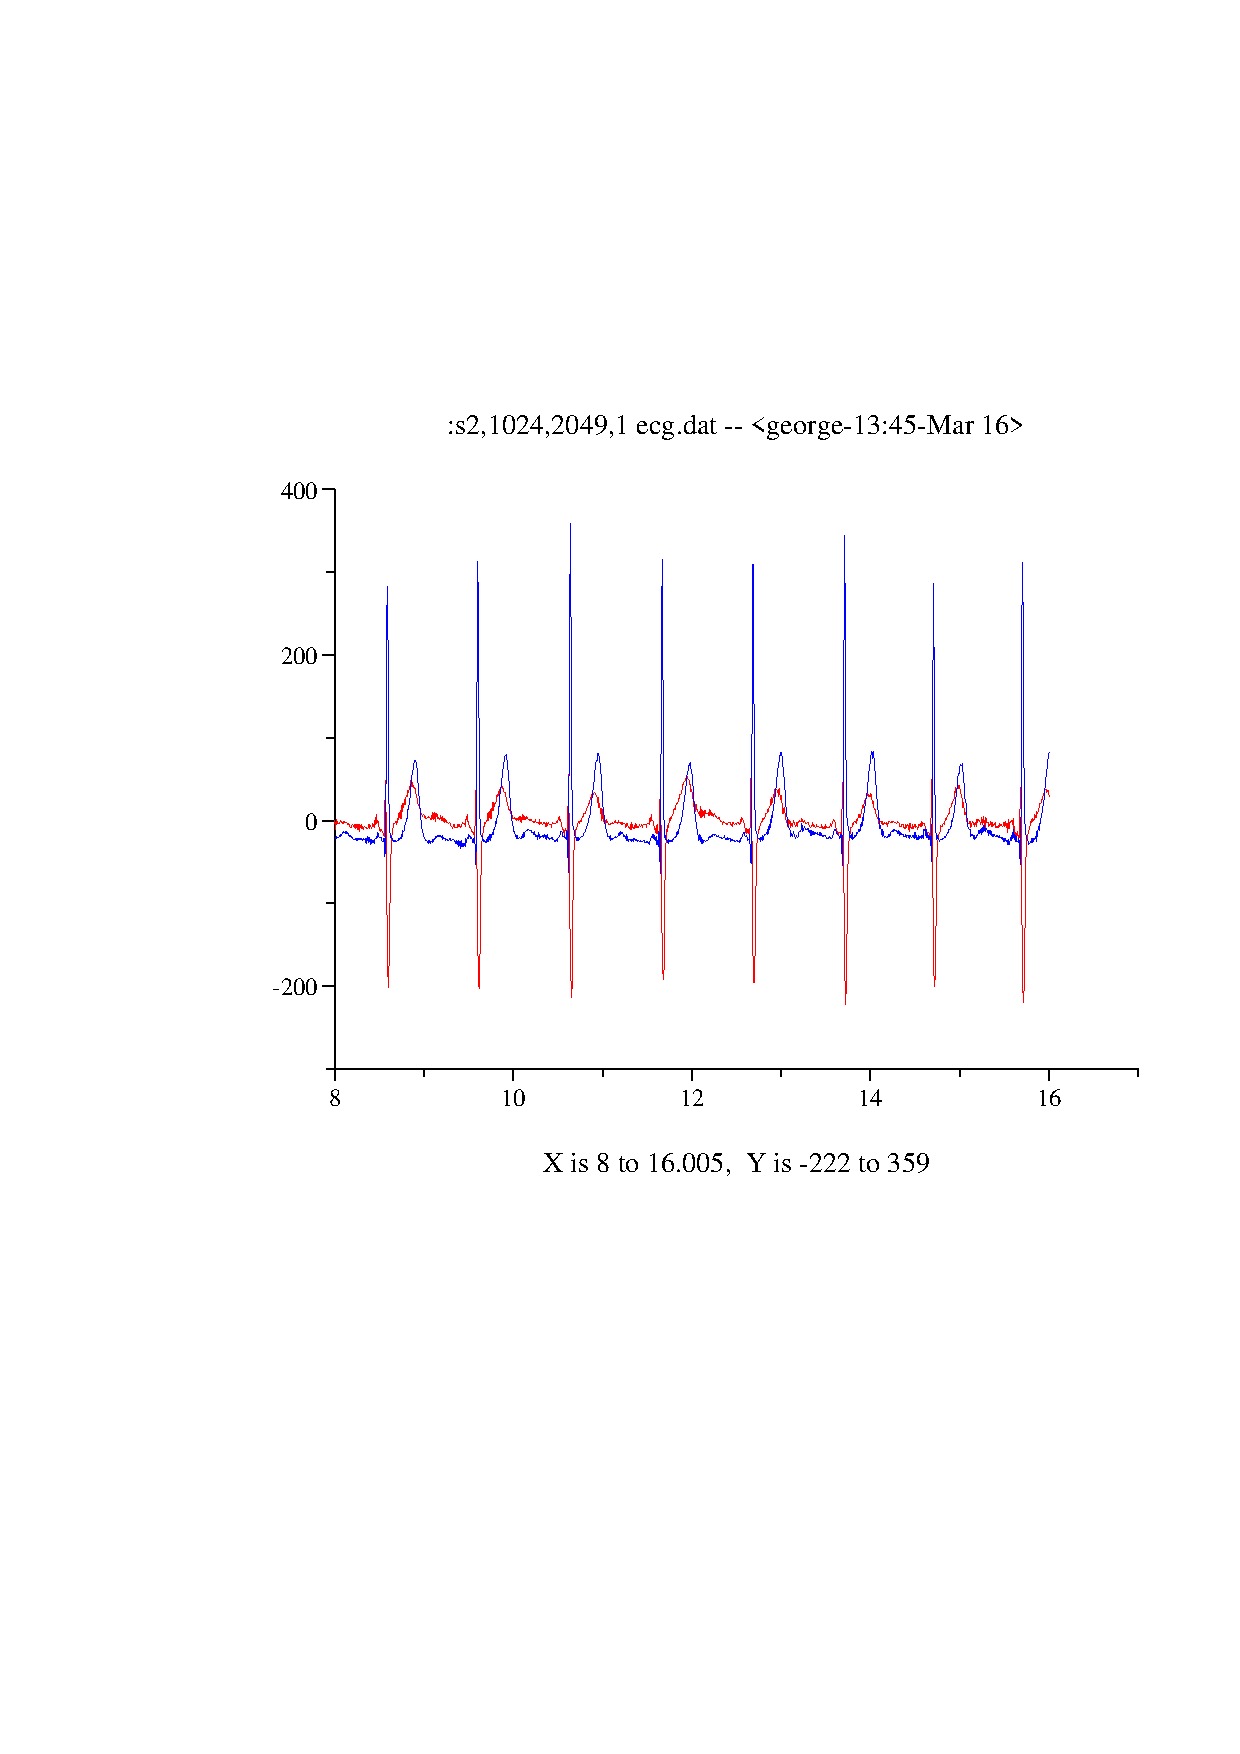
\epsfig{file=ecg,height=2cm}
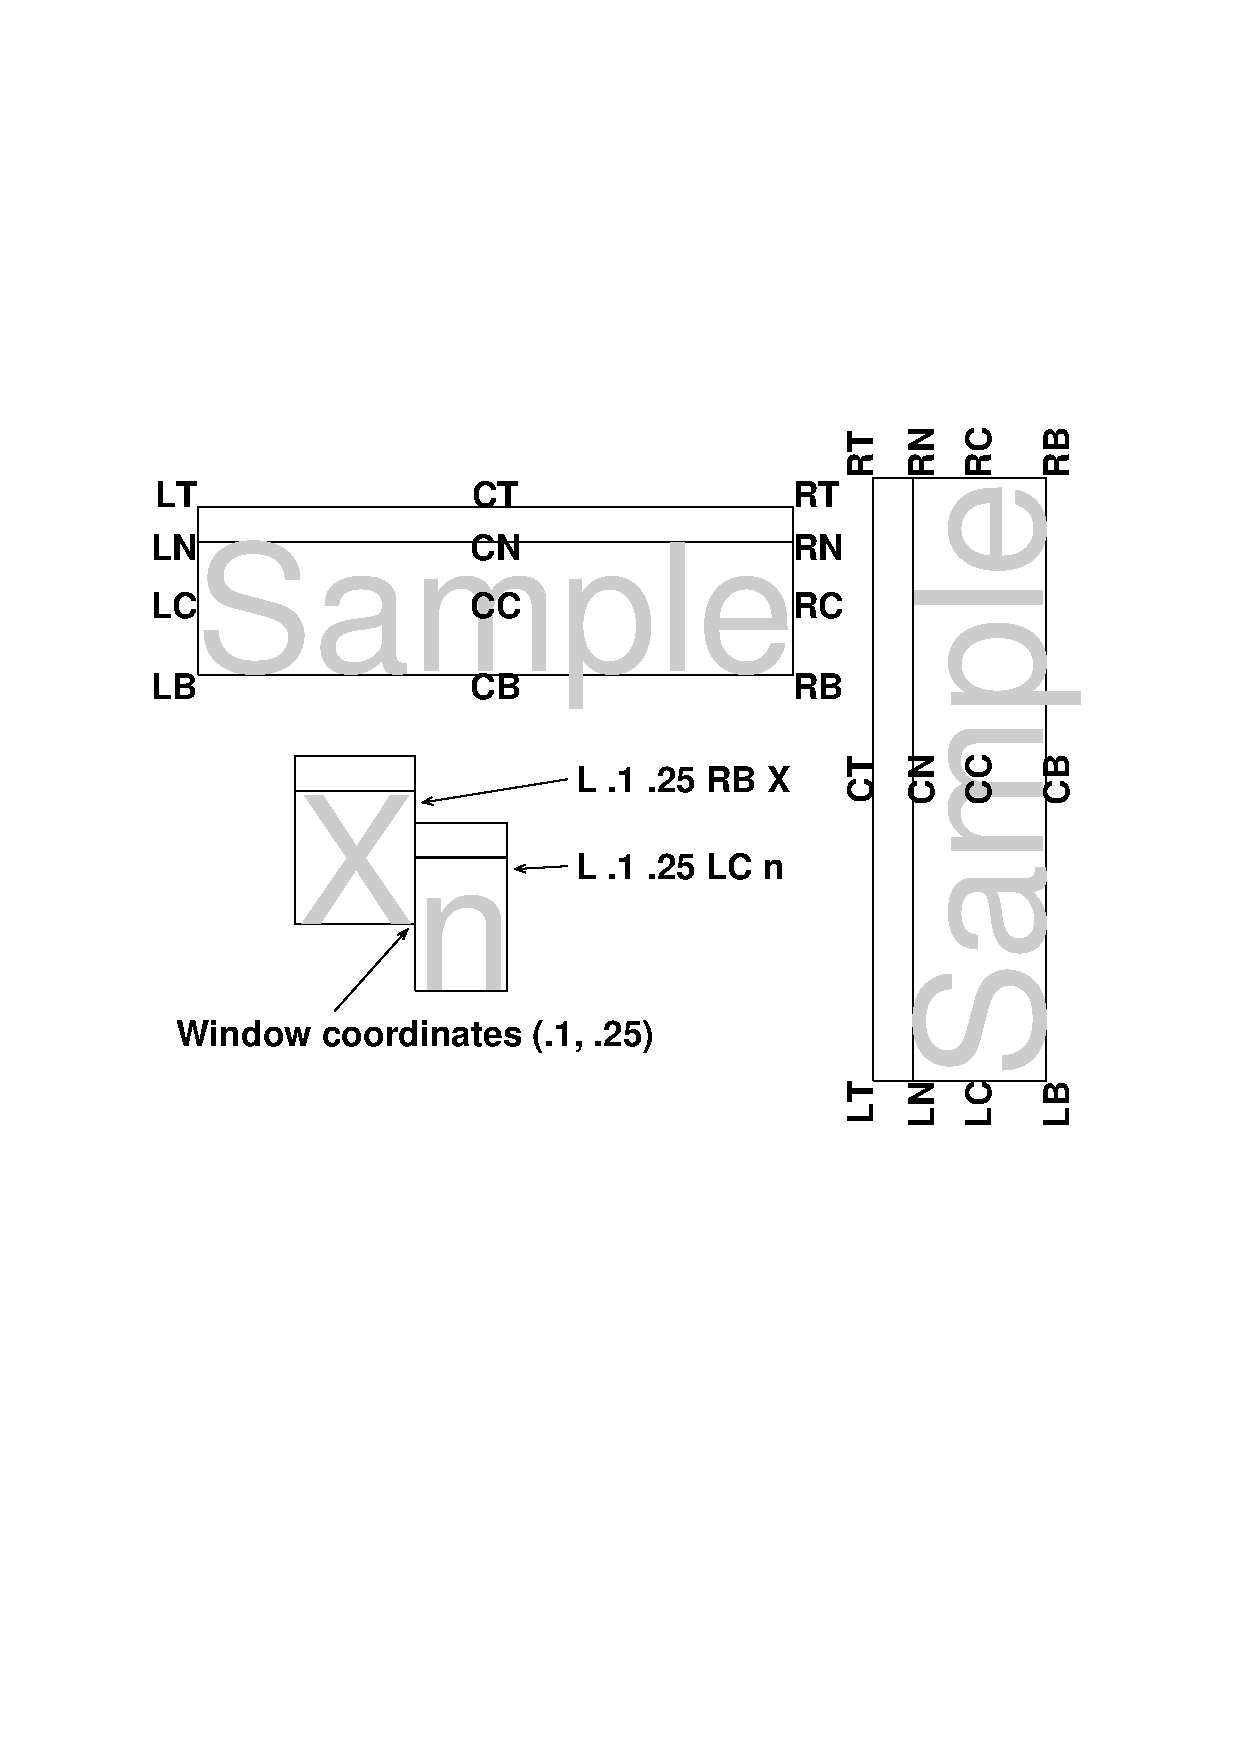
\epsfig{file=figure8,height=2cm}
\epsfig{file=colors,height=2cm}
\epsfig{file=figure14,height=2cm}
\vspace*{4cm}
\end{titlepage}
\thispagestyle{empty}

\vspace*{\fill}

\noindent
Copyright \copyright 2001--2005 George B. Moody.

\vspace{2cm}

\noindent
This copy of this book was prepared on \today{}.

\vspace{3mm}

\noindent
{\tt plt} was originally written by Paul Albrecht, and is currently
maintained by George Moody ({\tt george@mit.edu}).  The most recent
version of {\tt plt}, and of this book, can always be obtained from
PhysioNet ({\tt http://www.physionet.org/}); see
appendix~\ref{sec:distribution}, page~\pageref{sec:distribution}, for
details.

\vspace{3mm}

\noindent
Permission is granted to make and distribute verbatim copies of this
book provided that the copyright notice and this permission notice are
preserved on all copies.

\vspace{3mm}

\noindent
Permission is granted to copy and distribute modified versions of this
book under the conditions for verbatim copying, provided also that the
entire resulting derived work is distributed under the terms of a permission
notice identical to this one.

\vspace{3mm}

\noindent
Permission is granted to copy and distribute translations of this book into
another language, under the above conditions for modified versions.

\newpage
\setcounter{page}{1}
\tableofcontents

\newpage
\listoffigures

\chapter*{Acknowledgements}
\markboth{}{}

\index{Albrecht, Paul}%
\index{Stevenson, Kim}%
\index{Appel, Marvin}%
\index{Mietus, Joe}%
\index{pltmeister@\emph{pltmeister}}%
\index{plt Users' Guide@\emph{PLT USERS' GUIDE}}%
Thanks first to Paul Albrecht, for writing {\tt plt} and for making it
freely available in source form; and to Kim Stevenson and Marvin
Appel, who wrote the {\em PLT USERS' GUIDE} in 1988, which for many
years was the only available documentation for {\tt plt}, passed as
$n^{th}$-generation photocopies from user to user.  Significant
portions of chapters~\ref{sec:ax1}, \ref{sec:plotting-data},
\ref{sec:multiplots}, \ref{sec:labelling}, and~\ref{sec:ax2} are based
on Kim's and Marvin's guide, and many of the examples here are
reconstructed from their work.  Thanks also to the reviewers of
previous drafts of this book, and especially to Joe Mietus, {\em
pltmeister} of BIDMC.

I welcome your comments, corrections, and suggestions for improvements; please
send them to {\tt george@mit.edu}.

\chapter{Introduction}
\pagenumbering{arabic}

\index{Albrecht, Paul}%
\index{GNU/Linux}%
\index{Linux}%
\index{PostScript}%
\index{Unix}%
\index{X Window System}%
\index{pipe}%
This book describes {\tt plt}, a non-interactive plotting utility originally
written for Unix by Paul Albrecht.  {\tt plt} can produce publication-quality
2D plots in PostScript from easily-produced text or binary data files, and can
also create screen plots under the X Window System.  Compared to most other
software for 2D graphics, {\tt plt} has several significant advantages:

\begin{itemize}
\item
{\tt plt} generates compact vector PostScript output, which can be transmitted
quickly yet can be resized without introducing raster artifacts.

\item
{\tt plt} works well with a wide variety of tools that create and
manipulate readable text files.

\item
{\tt plt} is scriptable;  if you need to make 100 plots of 100 data sets,
you don't need to point and click for hours.

\item
Complex overlays and multi-part plots are easy to make, using multiple
invocations of {\tt plt} to write to a single window or page.

\item
{\tt plt} can read data from a pipe, so it can be used to observe real-time
signals or the outputs of computationally intensive processes as they become
available.

\item
{\tt plt} imposes no fixed limits on the number of points in a plot (even
the total amount of available memory is not a constraint if the data are
read from a pipe and the axis limits are pre-specified).

\item
{\tt plt} is free, open-source software that can be modified as needed for
unique applications.  ({\tt plt} can be compiled under GNU/Linux,
Mac OS X, MS-Windows, or any version of Unix.)

\item
{\tt plt} is easy to pronounce (say: P-L-T) and is almost as easy to spell :-)
\end{itemize}

\section{A brief history of {\tt plt}}

\index{Unix}%
\index{graph@{\tt graph}}%
\index{plot@{\tt plot}}%
\index{Albrecht, Paul}%
Early versions of Unix included an elegant utility called {\tt graph}, which
accepted simple text files such as:
\begin{center}
\begin{boxedverbatim}
1 1
2 4
3 9
4 16
\end{boxedverbatim}
\end{center}
\noindent
producing from them neatly scaled and labelled 2D plots in a device-independent
format.  {\tt graph} was accompanied by {\tt plot}, which consisted of a family
of interpreters (drivers) that translated {\tt graph}'s output for a wide
variety of mostly obsolete graphics terminals.  I wrote a number of {\tt plot}
drivers for slightly-less obsolete devices around 1982, and Paul Albrecht wrote
the first version of {\tt plt} as a replacement for {\tt graph} when it
disappeared from the standard Unix toolkit, sometime after Version 6.  (Try
it out: type the numbers above into a file named {\tt squares}, putting two
numbers on each line, then run the command ``{\tt plt squares}''.  It's that
easy!)

\index{PostScript}%
\index{X Window System}%
Early versions of {\tt plt} used drivers I had written for the Tektronix 4010
(a vector graphics terminal with a storage display; we had a few of them around
the lab), the Tektronix 4662 XY plotter that was capable of changing pens (the
first color output device we had), the NEC Spinwriter (an impact printer with
fine-resolution paper control, for which a special type wheel with a brass
``.'' was available, for plotting applications such as ours), and even dumb
terminals (with 80x24 resolution).  During the mid-1980s, MIT's Project Athena
produced the first versions of the X Window System, and Apple produced the
first PostScript printer (the LaserWriter).  Paul wrote X11 and PostScript
drivers and integrated them with {\tt plt}, in order to make better use of the
enhanced capabilities of these environments than was possible using only the
Unix {\tt plot} API.  It is these two drivers, with updates I have made since
the early 1990s, that are the nucleus of {\tt plt} today.

\section{How to read this book}

Stop!  Install the current version of {\tt plt} (see
appendix~\ref{sec:distribution}, beginning on
page~\pageref{sec:distribution}) if it is not already installed on
your system, or if the version you have already was installed before
\today{}.  Do this now, then come back here and read on.

This book attempts to be both a tutorial and a reference manual.  It
describes {\em every} {\tt plt} option, including many that have been
undocumented since {\tt plt} was written in the mid-1980s.  Although
you can read this book from cover to cover, in most cases you will not
need to do so in order to make high-quality plots.  {\tt plt} has a
bewildering number of options, but it is very easy to make simple
plots using only a small subset of these options.

If you have never used {\tt plt} before, begin with
chapter~\ref{sec:getting-started}, {\em Getting Started with {\tt plt}},
try out the examples there, and then try making a few plots of your
own before continuing.  Many readers will not need to go any further.

If you have used earlier versions of {\tt plt}, you may wish to look
first at appendix~\ref{sec:new}, {\em What's New?}, for a brief
summary of recent changes.

A good strategy for many users is to find in these pages an example
that illustrates features you would like to include in your plot, then
read the description of how the example was created.  In this sense,
this book is best used like a cookbook.  All of the scripts and data
files used to generate these examples are included in the {\tt doc}
subdirectory of the {\tt plt} distribution (see
appendix~\ref{sec:distribution}).

Chapter~\ref{sec:data-prep}, {\em Preparing Input for {\tt plt}}, is completely
new.  Even if you have been using {\tt plt} for years, you will probably find
some surprises here.  Chapter~\ref{sec:coord-systems} is also new; it contains
a systematic presentation of the four major coordinate systems (data, window,
page, and text) used by {\tt plt}.

Chapter~\ref{sec:ax1}, {\em Titles and Axes}, is essential reading if you have
not used {\tt plt} previously.  On the other hand, almost no one will need to
know everything in chapter~\ref{sec:plotting-data}, {\em Plotting Data}, but
it is worthwhile to skim through it, so that you will know what is possible.

Chapter~\ref{sec:multiplots}, {\em Plotting Two or More Data Sets Together},
will be helpful if you are trying to create a group of related plots; it
offers several ways to accomplish the task of presenting multiple data sets.

Often a few well-chosen text labels can clarify a plot;
chapter~\ref{sec:labelling}, {\em Labelling Your Plot}, shows how to make them.
Chapter~\ref{sec:lines-arrows}, {\em Drawing Line Segments, Arrows, and Boxes},
continues with the related subjects of adding arrows, outlined or shaded boxes,
and arbitrary line segments to your plots.

Occasionally you may need to prepare a plot without one or more of the standard
elements, such as axes or titles; chapter~\ref{sec:suppress}, {\em Suppressing
Plot Elements}, shows how to do this without using whiteout, as well as how to
include data points that fall outside of the axis ranges without inking them
in.

Throughout this book are examples that use a variety of line styles, shading,
color, and text fonts.  Chapter~\ref{sec:font-groups}, {\em Colors, Line
Styles, and Fonts}, discusses how to control these aspects of your plots'
appearance.

Chapter~\ref{sec:ax2}, {\em Advanced Axis Options} describes a variety of
special-purpose options for fine control over axes, including how to make
logarithmic axes and how to create extra labelled axis ticks.

\index{color}%
\index{GNU/Linux}%
\index{Linux}%
\index{PostScript}%
\index{Unix}%
\index{X Window System}%
At the end of this book, appendix~\ref{sec:color-names}, {\em Color Names},
contains a complete list of the named colors that can be used for PostScript
and X window output.  Appendix~\ref{sec:printed-output}, {\em Preparing Printed
Output}, contains details on creating printed plots on PostScript and other
printers, and on embedding plots in \LaTeX{} documents such as this one.
Appendix~\ref{sec:screen-output}, {\em On-Screen Plots}, describes how to use
{\tt plt} in an X Window System environment.  A few hints on writing shell
scripts with {\tt plt} appear in appendix~\ref{sec:scripting}, {\em Scripting
with {\tt plt}}.  Appendix~\ref{sec:distribution}, {\em How to get and install
{\tt plt}}, describes how to obtain {\tt plt} and how to compile and install
it.  Appendix~\ref{sec:new}, {\em What's New?}, summarizes new features in {\tt
plt}, and includes a (short) list of known bugs.  Finally,
appendix~\ref{sec:man-page} reproduces the {\tt man} page for {\tt plt}.
\newpage
\section{How to avoid reading this book\label{sec:quick}}

If you are temperamentally opposed to reading manuals, you may still
be able to figure out enough of {\tt plt} to use it from a quick look
at chapter~\ref{sec:getting-started}.  The {\tt doc} directory of the
{\tt plt} distribution contains two shell scripts:
\begin{itemize}
\item
{\tt xdemo.sh}, for generating and displaying the output of {\tt plt} in an X
  window.  Start your X server (use Cygwin/X under MS-Windows) before
  running {\tt xdemo.sh}.

\item
{\tt psdemo.sh}, for generating and displaying PostScript output from {\tt plt}
via {\tt gv} (freely available for Mac OS X from Fink, for MS-Windows from
Cygwin, or for GNU/Linux and Unix from SourceForge).  Other PostScript viewers
such as {\tt ggv} and {\tt gsview} can also be used (see {\tt gvcat} in the
{\tt src} directory).
\end{itemize}

Try out one or both of these scripts to see {\tt plt} in action, and
examine the scripts to see how they work.  Of course, this book is
always available when you need it!

\chapter{Getting Started with {\tt plt}\label{sec:getting-started}}

If you have never used {\tt plt}, this chapter contains the essential
information you need to begin making your own plots with {\tt plt}.  The first
section describes how {\tt plt} commands are constructed; don't skip this
section, because it introduces important concepts and terminology that are used
throughout the book.  A few notes on using {\tt plt} without an X server follow
in section~\ref{sec:nox}.  The chapter concludes with a tutorial,
section~\ref{sec:simple-plots}, in which you create a simple plot and then
produce several increasingly elaborate variations that illustrate a number of
the most useful features of {\tt plt}.  Be sure to work through these examples,
and then try making a few plots of your own before continuing.

\section{{\tt plt} Essentials\label{sec:essentials}}

\index{command syntax}%
\index{syntax, command}%
The general form of a {\tt plt} command is:
\begin{center}
\fbox{{\tt plt} {\em data-spec data-file column-number ... options}}
\end{center}

\index{column-number@{\em column-number}}%
\index{data-spec@{\em data-spec}}%
{\tt plt} recognizes its command-line arguments by looking at the
first character of each argument.  If an argument begins with ``{\tt
:}'', it's a {\em data-spec}.  If it begins with a digit (0-9), it's a
{\em column-number}; if it's either ``{\tt \#}'' or ``{\tt \%}'', it's
shorthand for ``all of the available column-numbers, in order.''  If
it begins with a hyphen ({\tt -}), it's an {\em option}.  If it begins
with ``{\tt (}'' (left parenthesis) or ``{\tt [}'' (left square
bracket), it's a {\em fontgroup specification} (not discussed further
in this section; see chapter~\ref{sec:font-groups}).  If the argument
begins with none of these special characters, it may be the name of a
{\em data-file}.

A {\em data-spec} is a string that describes the format of the {\em
data-file}.  Most plots do not require a {\em data-spec} (described in
section~\ref{sec:data-spec}), and you may omit this argument in such
cases.  If you provide a {\em data-spec}, it must precede the {\em
data-file} name in the command line.

The {\em data-file} contains the data you wish to plot, normally in
text format as columns of decimal numbers (other formats are described
in chapter~\ref{sec:data-prep}).  File {\tt example1.data} illustrates
the usual format:

\begin{center}
\begin{boxedverbatim}
0 0 0
1 1 2
2 3 1
3 5 3
4 7 2
\end{boxedverbatim}
\end{center}

\noindent
\index{pipe}%
This file contains three columns (from left to right: column numbers
0, 1, and 2) and five rows (from the top: row numbers 1, 2, 3, 4, and
5).  The {\em data-file}'s name, including the suffix if any, is
completely arbitrary; if the name of your {\em data-file} begins with
one of the special characters listed above, simply prefix it with
``{\tt ./}'' (since ``{\tt .}'' is always synonymous with the current
directory, ``{\tt ./anything}'' is an alternate name for ``{\tt
anything}'').  If you omit the name of the {\em data-file}, {\tt plt}
reads data from its standard input.  This feature allows you to pipe
data from another program into {\tt plt} without writing them to a
file first.

\index{column-number@{\em column-number}}%
You must specify at least one {\em column-number} (an integer $\ge 0$)
in order to plot data.  The column numbers must always follow the name
of the data file in the argument list (unless your data are supplied
via the standard input).  If you specify only one column number, {\tt
plt} assumes that the values it reads from that column are the y
values, and it either reads the x values from column 0 (if the data
file contains more than one column), or it generates a set of
successive integers, beginning with 0, to use as the x values by
default.

There are many {\em options} described in the following chapters.
Many of them accept or require additional arguments.  In most cases,
{\tt plt} can determine a reasonable default value for these
arguments.  If you supply a ``{\tt -}'' (hyphen) on the command line
in place of such an argument, {\tt plt} will choose a default.  In
this book, options normally follow the {\em data-file} and {\em
column-number} arguments on {\tt plt}'s command line.  This ordering
is not necessary in most cases, but this convention makes it easier
for humans to parse the command line.

\section{Using {\tt plt} without an X server \label{sec:nox}}

\index{GNU/Linux}%
\index{Linux}%
\index{Mac OS X}%
\index{MS-Windows}%
\index{Cygwin}%
The X Window System is a standard component of GNU/Linux and virtually
all current versions of Unix, including Mac OS X.  A high-quality
implementation of X is freely available for MS-Windows (Cygwin/X, from
{\tt http://www.cygwin.com/});  if you use MS-Windows, it will be well worth
the modest effort required to download and install an X server.  If you will
be using {\tt plt} with an X server, please skip ahead to
section~\ref{sec:more-options} below.

If you have not already installed {\tt plt}, please see
appendix~\ref{sec:distribution}, beginning on page~\pageref{sec:distribution}.

\index{PostScript}%
\index{gv}%
\index{GSView}%
{\tt plt} can generate PostScript plots, which can be printed directly on
PostScript printers or (via {\tt ghostscript}) on a variety of non-PostScript
printers.  {\tt ghostscript} can also render PostScript on-screen, but this
is most easily managed using a GUI wrapper such as {\tt gv}, {\tt ggv},
{\tt mgv}, {\tt ghostview}, or {\tt GSView}.  All of these require an X server,
except that GSView can use native graphics when running on MS-Windows or OS/2.
See {\tt http://\-www.\-cs.\-wisc.\-edu/\-~ghost/\-gv/} for details on these
GUI wrappers for {\tt ghostscript}.

\index{lwcat}%
When using {\tt plt} without an X server running, always send the output to
{\tt lwcat}.  There are two ways to do this:

\index{pipe}%
\begin{enumerate}
\item
Send the output via a pipe, as in ``{\tt plt ... | lwcat}''.  (This is
the recommended method.)

\item
Collect the output in a file, as in ``{\tt plt ... $>$output.plt}'',
then read the file, as in ``{\tt lwcat $<$output.plt}''.   Note that
the output file does not contain a PostScript prolog, so it cannot be
printed directly;  {\tt lwcat} is responsible for adding the prolog.
\end{enumerate}

\index{Cygwin}%
\index{GhostScript}%
You can easily follow along with all of the examples in this book, which work
using the PostScript driver in exactly the same way as when using the X driver,
if you simply add ``{\tt |~lwcat -gv}'' to the end of each {\tt plt} command.
(You may omit ``{\tt -gv}'' if you are running within a Cygwin/bash window
under MS-Windows.)  When you do this, the output of {\tt plt} is opened in a
{\tt gv} or GSView window.  Using {\tt gv} or GSView's controls, you can save
the plot as a file, print it (on any printer supported by GhostScript, not just
on PostScript printers), and view it at natural or magnified scales.  (Drivers
for a vast range of printers are included with GhostScript; see {\tt
http://www.ghostscript.com/} for a list of supported printers.)

\vspace{5mm}
{\small
You might reasonably wonder why {\tt lwcat} is not part of {\tt plt}.  The
reason is that the output of several {\tt plt} commands can be concatenated
and supplied to {\tt lwcat} in a single batch to create multiple plots on
a single page (see chapter~\ref{sec:multiplots}).  To do this,
group the {\tt plt} commands together within a pair of parentheses, separating
them with newlines or semicolons;  then send the output of the entire group
to {\tt lwcat}, either like this:

\begin{center}
\begin{boxedverbatim}
( plt data1 ... ; plt data2 ...; plt data3 ... ) | lwcat
\end{boxedverbatim}
\end{center}

\noindent
or like this:

\begin{center}
\begin{boxedverbatim}
( plt data1 ... ; plt data2 ...; plt data3 ... ) >output.plt
lwcat <output.plt
\end{boxedverbatim}
\end{center}

If you are paying particularly close attention while reading the rest of
this book, you may notice that {\tt plt} accepts the option {\tt -T lw}
to specify PostScript output.  If an X server is not running, this is
the default, so that the {\tt -T lw} option can be omitted.  Furthermore,
{\tt lwcat} accepts the option {\tt -gv} to specify that the output is to
be opened using {\tt gv} (GSView under MS-Windows), but this is the default
if you are running {\tt plt} and {\tt lwcat} in a Cygwin/bash window, so
that the {\tt -gv} option can be omitted in this case.  If you attempt to
run {\tt plt} and {\tt lwcat} under MS-Windows in a DOS window (which is
not recommended), or in some other way (also not recommended), you will need
to use the {\tt -gv} option explicitly.
}% (end of \small)

\section{More about options \label{sec:more-options}}
\index{command-line help}%
\index{help}%
\index{h@{\tt -h} (help) option}%
One of the most useful options is {\tt -h}, which causes {\tt plt} to
print a (very) concise summary of its options on the standard output.
Since there are many options, the output of ``{\tt plt -h}'' will scroll
off of your screen, so you may wish to send it to {\tt more} (or a similar
pager): 
\begin{center}
\begin{boxedverbatim}
plt -h | more
\end{boxedverbatim}
\end{center}

If the {\tt -h} option is followed by one or more strings (which should not
begin with hyphens), {\tt plt} prints one-line summaries of all
options beginning with those strings only.

\index{f@{\tt -f} (format file) option}%
As an alternative to supplying options and their arguments on the
command line, you may write them into a {\em format file} that can
be read by {\tt plt}.  This facility is particularly useful when you
create a series of complex plots using some or all of the same
options.  You can put some of your options in a format file and supply
others on the command line.  Within a format file, omit the initial
hyphen ({\tt -}) from each option name.  To use a format file, supply
the option {\tt -f} followed by the name of the format file, as in:

\begin{center}
\begin{boxedverbatim}
plt data-file 0 1 -f format-file
\end{boxedverbatim}
\end{center}

\index{F@{\tt -F} (format string) option}%
A third way to pass options to {\tt plt} is within a quoted {\em format
string}, following the {\tt -F} option.  Use the same syntax in a
format string as in a format file.
For examples of {\tt -f} and {\tt -F}, compare
figures~\ref{fig:example3} and~\ref{fig:example4} on
pages~\pageref{fig:example3} and~\pageref{fig:example4}.

Let's see how a simple plot can be created, using {\tt example1.data}.
If we would like the first column to be the set of x coordinates and the
third column to be the set of y coordinates, we can type:
\begin{center}
\begin{boxedverbatim}
plt example1.data 0 2
\end{boxedverbatim}
\end{center}
and our plot would look like figure~\ref{fig:example1}.

\begin{figure}[!h]
\begin{center}
\begin{tabular}{p{10cm}p{1.5cm}}
\fcolorbox{blue}{white}{
\epsfig{file=figure1,height=8cm}} &
{\vspace{-8cm}
{\em Data}
\vspace*{3mm}

\begin{boxedverbatim}
0 0 0
1 1 2
2 3 1
3 5 3
4 7 2
\end{boxedverbatim}
}
\end{tabular}
\end{center}
\caption[A simple plot]{Produced using the command: \label{fig:example1}}
\begin{center}
\begin{boxedverbatim}
plt example1.data 0 2
\end{boxedverbatim}
\end{center}
\index{bounding box}%
To see how to include {\tt plt} output as a figure in a \LaTeX{}
document such as this one, refer to appendix~\ref{sec:latex},
\emph{Including {\tt plt} figures in a \LaTeX{} document},
page~\pageref{sec:latex}.  The frame lines surrounding most of the
figures in this book show their bounding boxes (corresponding to
the borders of the {\tt plt} window for an on-screen plot, or of
the page for a printed plot.)
\end{figure}

\index{column-number@{\em column-number}}%
Notice that in the command line, the argument ``{\tt 0}'' corresponds
to the first column of {\tt example1.data}, and the argument ``{\tt
2}'' to the third column.  Column 0 becomes the x axis;  column 2
becomes the y axis.  Likewise, the argument ``{\tt 1}'' in either of
these two positions would correspond to column 1 (the second column)
of {\tt example1.data}, and would become either the x or the y axis
depending upon its position.

\index{PostScript}%
{\tt plt} can produce both screen and printed plots.  If you try the
examples exactly as shown in the main part of this book, you will
obtain screen plots.  Although you can use other software to make and
print screen dumps of these plots, this is neither the best nor the
easiest way to print your plots on paper.  The following sections show
how you can obtain publication-quality plots on PostScript or other types
of printers, with only minor changes to the {\tt plt} commands needed
to make the corresponding screen plots.

\section{Tutorial: Simple Plots \label{sec:simple-plots}}

Please try out the examples shown below (and throughout this book) on
your own computer.   You can find the necessary input files in the
{\tt doc} directory of the {\tt plt} distribution (where you will also
find the \LaTeX{} sources for this book, and a printable PostScript
version of it).  For this tutorial, you will need only one file from
the {\tt plt} distribution, a text data file named {\tt heartrate.data},
which begins:

\begin{center}
\begin{boxedverbatim}
6.46389 58.0645
7.49722 59.0164
8.51389 63.3431
9.46111 65.2568
10.3806 57.2944
11.4278 57.754
\end{boxedverbatim}
\end{center}

\index{column-number@{\em column-number}}%
As the excerpt above shows, {\tt heartrate.data} contains two columns
of numbers;  in all, there are 297 rows (lines) in the file.  The
numbers on the left (in column 0) represent elapsed time in seconds, and
those on the right (in column 1) indicate instantaneous heart rate in
beats per minute.  (See {\tt doc/Makefile} in the {\tt plt}
distribution if you are interested in knowing more about these data.)

\subsection{Screen and printed plots}

The simplest way to plot these data is to type this command into a
terminal window:

\begin{center}
\begin{boxedverbatim}
plt heartrate.data
\end{boxedverbatim}
\end{center}

\index{overlays}%
\index{xpltwin@{\tt xpltwin}}%
A new window will open, containing a plot as in
figure~\ref{fig:simple0}.  You may be surprised to see {\tt plt} exit
to the shell prompt while the window containing the plot remains
on-screen.  If you run {\tt plt} again, it will draw its output into
the same window as the first.  This feature allows you to create
complex overlaid plots using several invocations of {\tt plt}, as
described in chapter~\ref{sec:multiplots}, beginning on
page~\pageref{sec:multiplots}.  To dismiss the window, type an {\sf
Esc} (or {\tt Q}, or {\tt X}) into it.  (If you wish to look at two or
more plots in separate windows, open a new window for {\tt plt} using
{\tt xpltwin}; see appendix~\ref{sec:screen-output}, beginning on
page~\pageref{sec:screen-output}, for details). The same capability
for creating overlays is also available when producing printed output;
see appendix~\ref{sec:printed-output}, beginning on
page~\pageref{sec:printed-output}, for details.

In order to illustrate the appearance of a {\tt plt} screen plot,
figure~\ref{fig:simple0} was prepared from a screen dump.  You can
make printed plots of much better quality using {\tt plt}, however,
and with much less trouble than required to print a screen dump.  The
same plot can be printed simply by adding the optional arguments
``{\tt -T lw}'' to the {\tt plt} command, and then redirecting its
output to {\tt lwcat}, like this:

\begin{center}
\begin{boxedverbatim}
plt heartrate.data -T lw | lwcat
\end{boxedverbatim}
\end{center}

This command will send the plot to the default printer, producing
output as in figure~\ref{fig:simple1}.  Since PostScript plots are
in vector rather than raster form, they can be rescaled in documents
such as this without introducing artifacts, and their resolution is
generally much higher than raster images despite their much smaller file
sizes.

If you wish to capture the PostScript output in order to include it in
a document such as this one, use {\tt lwcat}'s {\tt -eps} option, and
redirect its standard output to a file, as in:

\begin{center}
\begin{boxedverbatim}
plt heartrate.data -T lw | lwcat -eps >heartrate.eps
\end{boxedverbatim}
\end{center}

See appendix~\ref{sec:printed-output} for more examples and additional
details about making PostScript plots and including them in other
documents.

\begin{figure}
\begin{center}
\epsfig{file=simple0,height=8cm}
\caption{Simple screen plot \label{fig:simple0}}
\end{center}
\end{figure}
\begin{figure}
\begin{center}
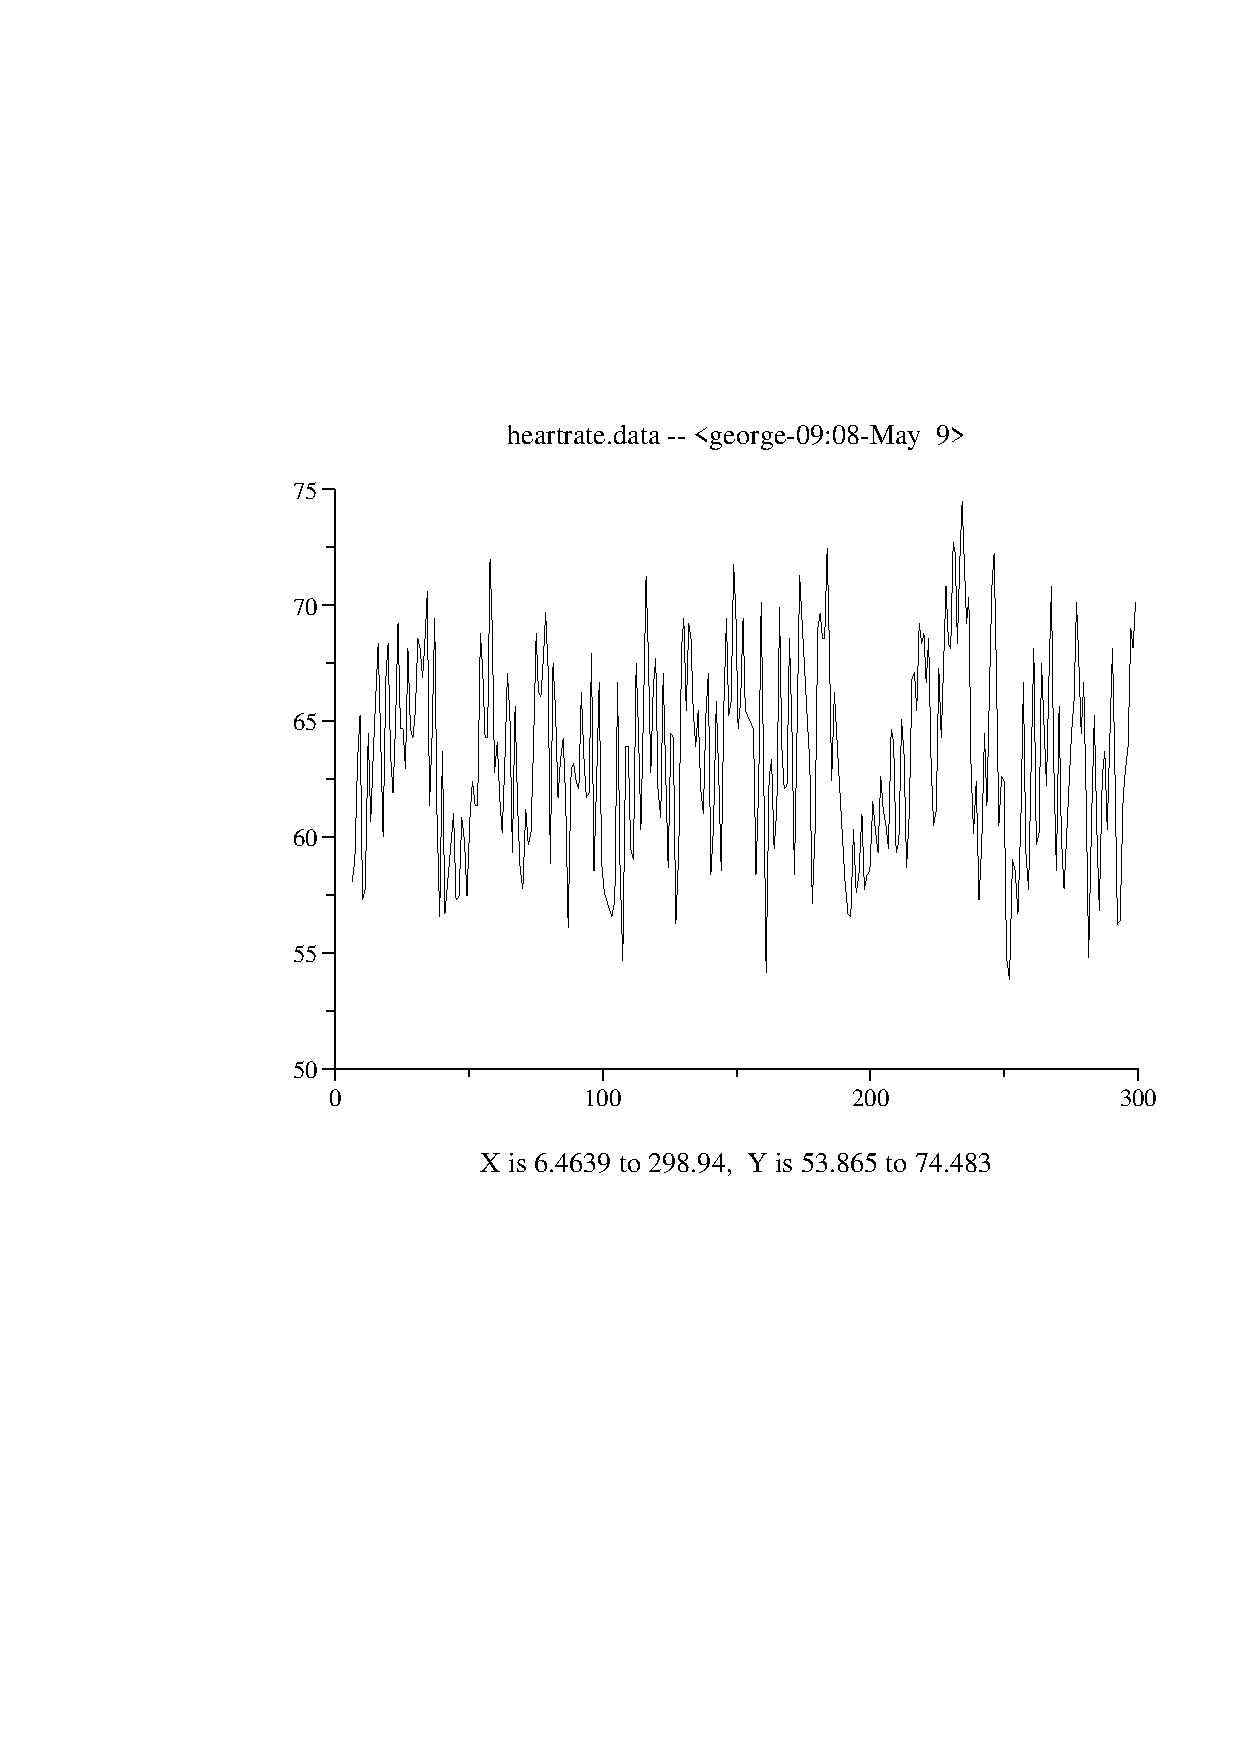
\epsfig{file=simple1,height=8cm}
\caption{Simple printed plot \label{fig:simple1}}
\end{center}
\end{figure}

\subsection{Adding titles and axis labels}

Now that we know how to make simple screen and printed plots, let's
refine the plot a bit.  First, we can provide a title for the plot,
and for the x and y axes using the {\tt -t}, {\tt -x}, and {\tt -y}
options, like this:

\begin{center}
\begin{boxedverbatim}
plt heartrate.data -t "Heart rate time series" \
  -x "Time (seconds)" -y "Heart rate (beats per minute)"
\end{boxedverbatim}
\end{center}

\noindent
(The ``{\tt $\backslash$}'' at the end of the first line means that the
command is continued on the next line; you may enter the command on
two lines, ending the first with a backslash, or you may combine both
lines into one, omitting the backslash.)

This command produces the neatly labelled version of the plot shown in
figure~\ref{fig:simple2}.  This and all of the later figures in this
book were prepared as PostScript plots, using {\tt plt}'s ``{\tt -T
lw}'' option and piping the output to {\tt lwcat} as in
figure~\ref{fig:simple1}.  Except in the discussion of printed output in
appendix~\ref{sec:printed-output}, however, the {\tt plt} commands
shown here omit ``{\tt -T lw | lwcat}'', so that they can be
used to make screen plots.

\begin{figure}
\begin{center}
\epsfig{file=simple2,height=8cm}
\caption{Simple plot with titles and axis labels \label{fig:simple2}}
\end{center}
\end{figure}

\subsection{Setting up the axes}

As you may have noticed, {\tt plt} chose appropriate ranges for the x
and y axes based on the ranges of x and y values in its input.  Often,
you may wish to specify the axis ranges, however, particularly if
several plots are to be compared (in which case the plots should be
prepared with the same scales and axis ranges).  The next version of
our plot, shown in figure~\ref{fig:simple3}, illustrates the {\tt -xa}
and {\tt -ya} options for setting up the axes:

\begin{center}
\begin{boxedverbatim}
plt heartrate.data -t "Heart rate time series" \
  -x "Time (seconds)" -y "Heart rate (beats per minute)" \
  -xa 60 300 15 - 4 0 -ya 0 80 20 -g grid,sub
\end{boxedverbatim}
\end{center}

\begin{figure}
\begin{center}
\epsfig{file=simple3,height=8cm}
\caption{Simple plot with customized axes and grid \label{fig:simple3}}
\end{center}
\end{figure}

The {\tt -xa} and {\tt -ya} options each take an argument list
containing up to six arguments.  In this example, the argument list
for {\tt -xa} is ``{\tt 60 300 15 - 4 0}'', and that for {\tt -ya}
is ``{\tt 0 80 20}'' ({\tt plt} recognizes {\tt -g} as another option,
rather than as part of {\tt -ya}'s argument list, because {\tt -g}
consists of a hyphen followed by a letter).

The first two arguments following {\tt -xa} and {\tt -ya} specify the
x and y axis ranges.  Notice that the x axis range (60 to 300)
excludes a number of the points at the beginning of the data file.  If
you try this command, {\tt plt} will warn you (by printing a message
in your terminal emulator window) that points were excluded from the
plot;  note that there is no indication of this on the plot itself,
however.

The third argument following each of {\tt -xa} and {\tt -ya} specifies
the interval between axis ticks (in the units of the data).  We have
chosen 15 units for the x axis tick interval, since the x units are
seconds and this allows us to arrange for a numbered tick at the
beginning of each minute (the {\tt 4} following {\tt -xa} specifies
that every fourth tick is to be numbered).

The ``{\tt -}'' between the {\tt 15} and the {\tt 4} is an example of
a {\em default argument}.  In most cases, where {\tt plt} expects an
argument, it will choose a reasonable default if you provide ``{\tt
-}'' instead of a specific value.  The value that ``{\tt -}'' replaces
in this case is a format string that can be used to control how the
numbered x axis ticks are printed.  Note that, as in the argument list
for {\tt -ya} in this example, it is also usually acceptable to omit
arguments at the end of a list if {\tt plt}'s defaults are acceptable
to you.  For further details on using the
{\tt -xa} and {\tt -ya} options, see chapter~\ref{sec:ax1}.

The {\tt -g} option and its argument ({\tt grid,sub}) specifies that
{\tt plt} should draw gridlines across the plot at every axis tick.
See chapter~\ref{sec:ax2} for details about using {\tt -g} to control
the appearance of the grid.

\subsection{A simple scatter plot}

In the figures above, the data are plotted by connecting the points
with straight line segments.  This is {\tt plt}'s default plot style,
and for many plots, it is adequate.  For {\tt heartrate.dat},
however, a scatter plot may be a more appropriate format.  The next
version of our plot adds the option ``{\tt -p 0,1Scircle}'' to the {\tt
plt} command in order to create a scatter plot, as shown in
figure~\ref{fig:simple4}:

\begin{center}
\begin{boxedverbatim}
plt heartrate.data -t "Heart rate time series" \
  -x "Time (seconds)" -y "Heart rate (beats per minute)" \
  -xa 60 300 15 - 4 0 -ya 0 80 20 -g grid,sub \
  -p 0,1Scircle
\end{boxedverbatim}
\end{center}

\begin{figure}
\begin{center}
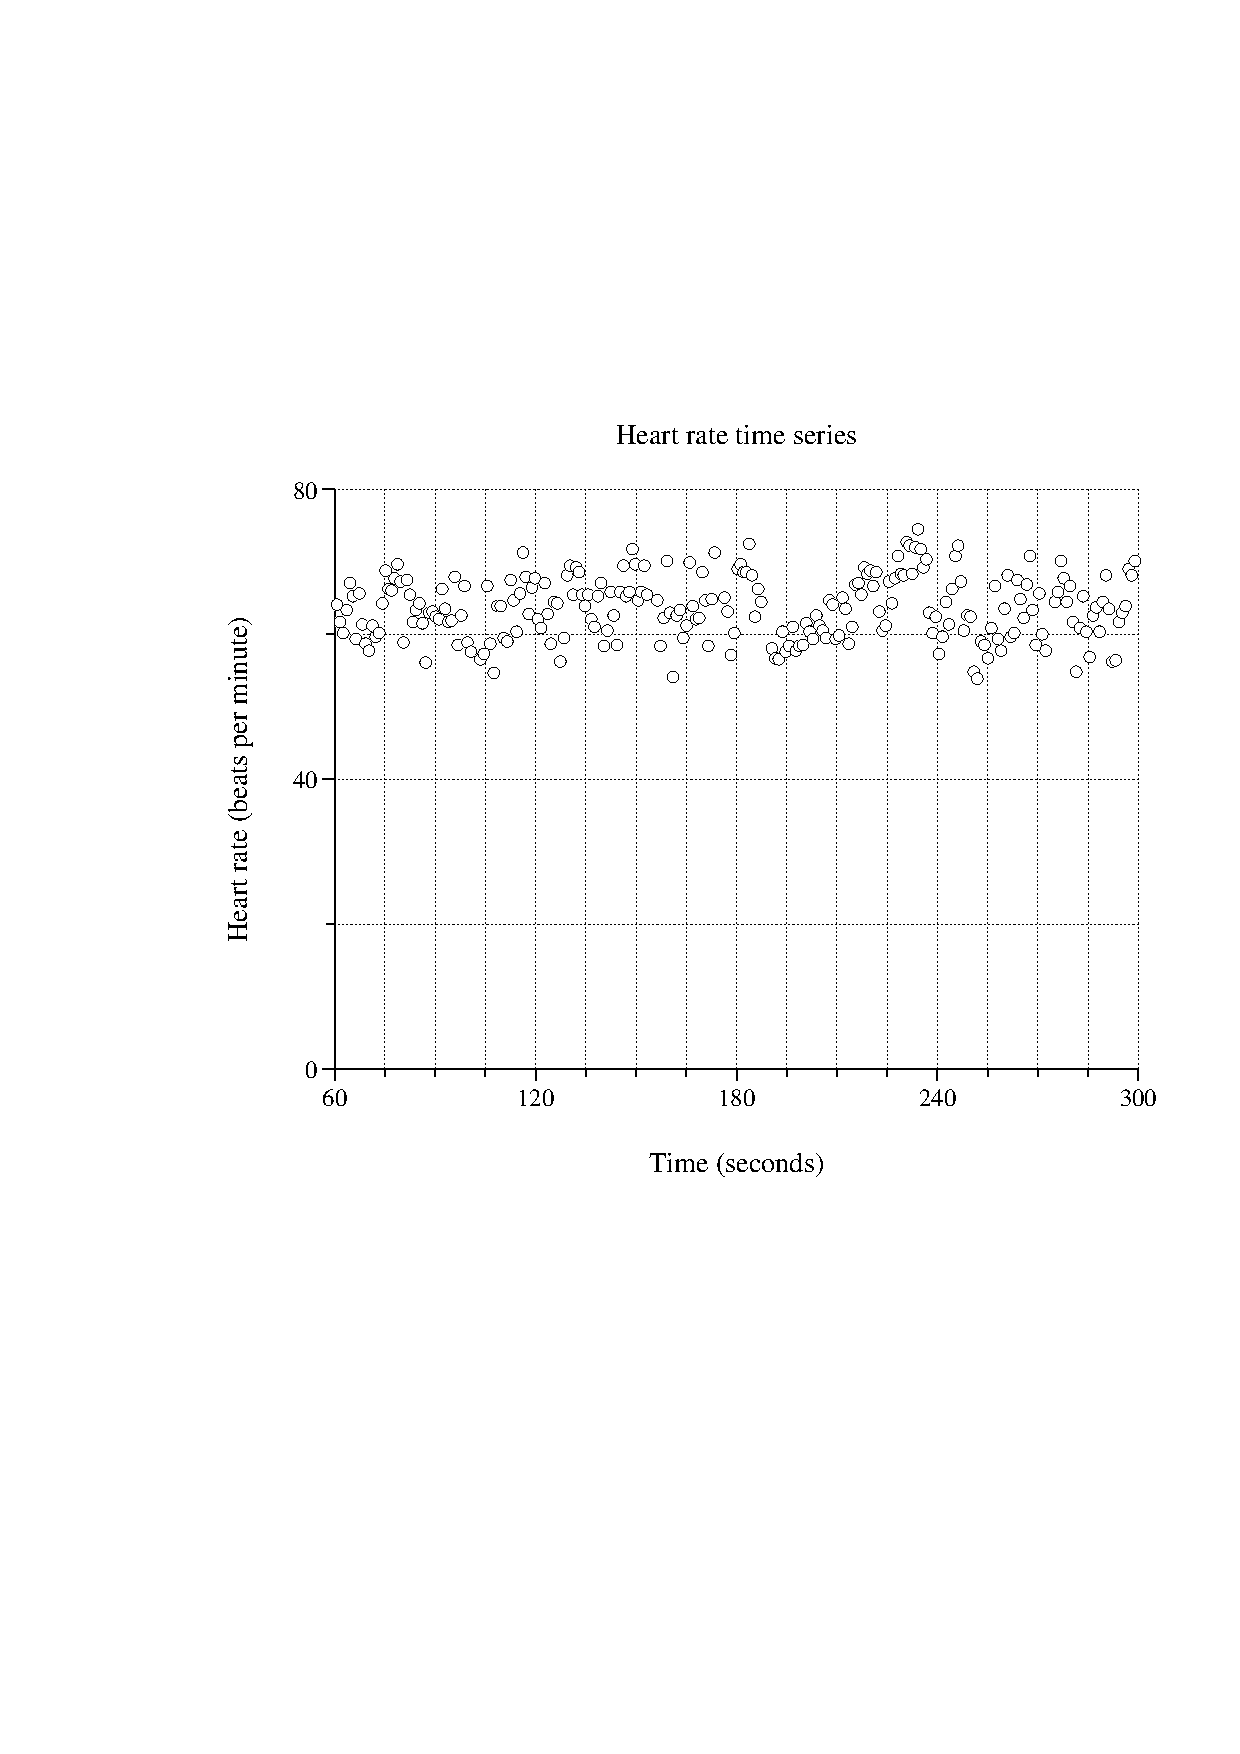
\epsfig{file=simple4,height=8cm}
\caption{Scatter plot \label{fig:simple4}}
\end{center}
\end{figure}

The use of the {\tt -p} option to specify a plot style is described in
chapter~\ref{sec:plotting-data};  {\tt plt} offers a wide range of
styles.  The argument ``{\tt 0,1Scircle}'' specifies that columns 0 and 1
of the data are to be used to make a plot in style {\tt S} (a
scatter plot) using an open circle to mark each data point.

\subsection{Using color}

We conclude this tutorial by adding a {\em transient
fontgroup specification} (see chapter~\ref{sec:font-groups}) that has
the effect of modifying the appearance of the scatter plot symbols.
To do this, we append ``{\tt (P/2,Cblue)}'' to the argument of the
{\tt -p} option, like this:

\begin{center}
\begin{boxedverbatim}
plt heartrate.data -t "Heart rate time series" \
  -x "Time (seconds)" -y "Heart rate (beats per minute)" \
  -xa 60 300 15 - 4 0 -ya 0 80 20 -g grid,sub \
  -p "0,1Scircle(P/2,Cblue)"
\end{boxedverbatim}
\end{center}

\begin{figure}
\begin{center}
\epsfig{file=simple5,height=8cm}
\caption{Scatter plot in color \label{fig:simple5}}
\end{center}
\end{figure}

(Since the shell (command interpreter) normally treats parentheses as
special characters, it is necessary to enclose the entire argument of
{\tt -p} in quotation marks, in order to pass it as shown to {\tt plt}
without shell interpretation.)

Fontgroup modifications provide an extremely powerful and flexible way to
control the appearance of a plot.  In this example, ``{\tt P/2}''
reduces the size of the circles by a factor of 2, and ``{\tt Cblue}''
causes them to be drawn in blue.  (A complete list of color names is
included in appendix~\ref{sec:color-names}.)

\section{Plotting an image}

\index{image plots}%
\index{greyscale images}%
The {\tt plt} package includes a tiny program named {\tt imageplt} that
can be used together with {\tt plt} to plot a greyscale image, as shown
in figure~\ref{fig:image}.  The input to {\tt imageplt} should be a list
of grey levels (0 = black, 1 = white) for each pixel in the image, beginning
at the lower left corner, going up each column, then continuing from the
bottom of the next column, etc.  For example, suppose the input file
{\tt image.data} contains:

\begin{center}
\begin{boxedverbatim}
1 .9 .8 .7 .6
0 0 0 0 0
1 1 1 1 1
\end{boxedverbatim}
\end{center}

These data can be plotted as a 3x5 image to produce
figure~\ref{fig:image}.  For further details, see
Appendix~\ref{sec:man-page}.

\begin{figure}[h]
\begin{center}
\fcolorbox{blue}{white}{
\epsfig{file=image,height=10cm}}
\end{center}
\caption[Using imageplt]{Produced using the command: \label{fig:image}}
\begin{center}
\begin{boxedverbatim}
imageplt -d 5 3 image.data | plt 0 1 2 -pc
\end{boxedverbatim}
\end{center}
\end{figure}

\section{Plotting a function of a single variable}

\index{function plots}%
{\tt plt} plots {\em (x, y)} coordinate pairs, but often you may wish
to plot a continuous function of {\em x} expressed symbolically.  This
can be done easily using two small programs, {\tt ftable} and {\tt
pltf}, both of which are included with {\tt plt}.

Both of these programs accept a symbolic function definition (as the
first command-line argument) and up to three optional arguments:
the lower and upper bounds for the independent variable (which is
always {\tt x}), and the {\tt x}-increment.

{\tt ftable} produces a script that generates a table of coordinate
pairs when processed by the standard {\tt bc} utility.  This table can
then be used as input to {\tt plt}.  For example, the command:

\begin{center}
\begin{boxedverbatim}
ftable 'x^2 - 4*x + 7' 0 5 .1 | bc -l
\end{boxedverbatim}
\end{center}

\noindent
produces on its standard output a table of values of the function
$f(x)=x^2-4x+7$ for values of $x$ between 0 and 5, with a step
size of .1 in $x$.  Note that the independent variable in the function
is always {\tt x}, and that multiplication must be indicated
explicitly using {\tt *}.  In this example, the output begins like this:

\begin{center}
\begin{boxedverbatim}
0 7
.1 6.61
.2 6.24
.3 5.89
.4 5.56
.5 5.25
.6 4.96
.7 4.69
\end{boxedverbatim}
\end{center}

\index{bc}%
\index{GNU/Linux}%
\index{Linux}%
\index{Mac OS X}%
\index{MS-Windows}%
\index{Cygwin}%
\index{Fink}%
The {\tt bc} utility is an arbitrary-precision calculator included in
all versions of Unix and GNU/Linux, and available for Mac OS X (from
{\tt http://fink\-.source\-forge\-.net/}) and for MS-Windows (as part
of the free Cygwin package from {\tt http://www\-.cyg\-win\-.com/}).
See the documentation for {\tt bc} for details on the function syntax.

\index{pltf}%
\index{ftable}%
The shell script {\tt pltf} is included in the {\tt misc} directory of
the {\tt plt} distribution.  {\tt pltf} accepts the same arguments as
{\tt ftable} (the function, the lower and upper bounds for {\tt x},
and the {\tt x}-increment), but it invokes {\tt bc} and {\tt plt} to produce
a neatly labelled plot of your function, as illustrated in
figure~\ref{fig:function}:

\begin{center}
\begin{boxedverbatim}
pltf 's(40*x)*s(3*x)' 0 5 .01
\end{boxedverbatim}
\end{center}

\begin{figure}
\begin{center}
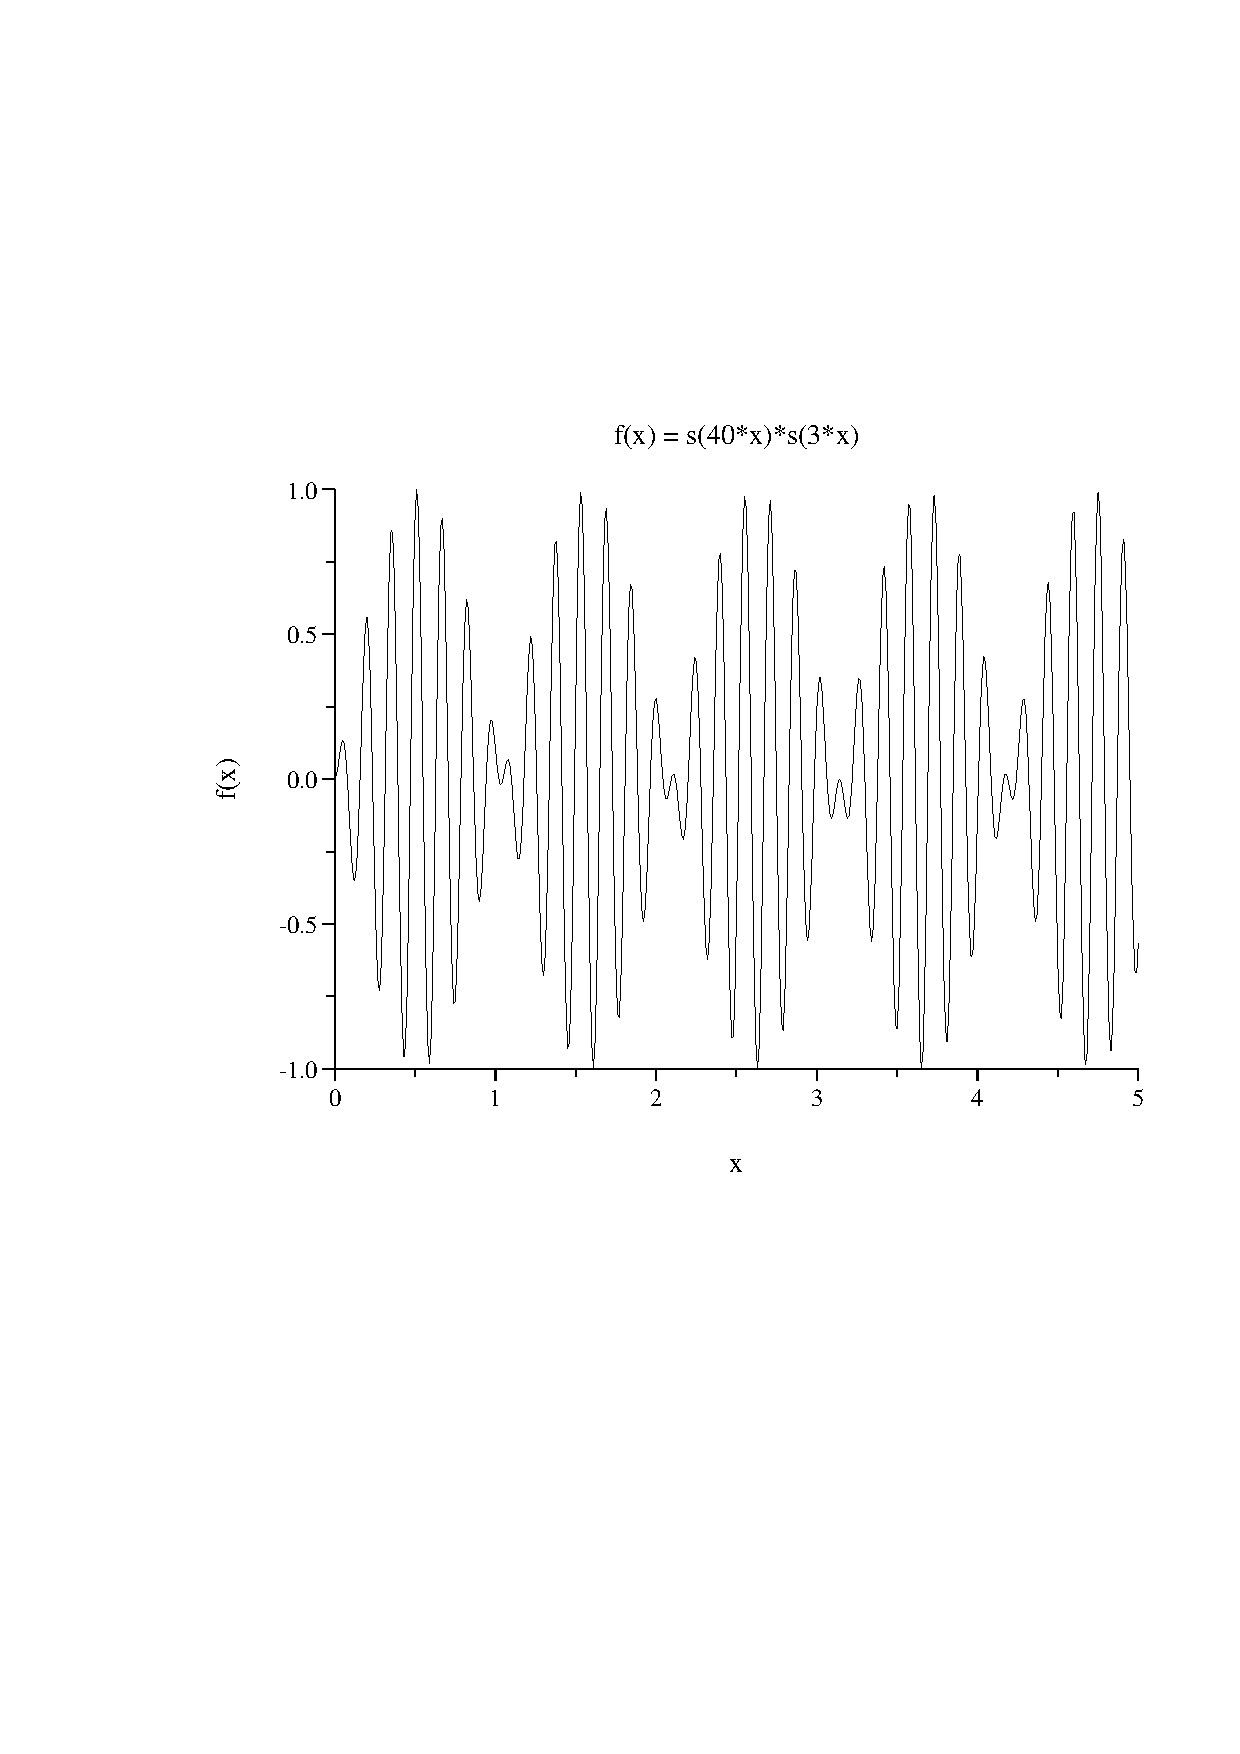
\epsfig{file=function,height=8cm}
\caption{Function plot made using {\tt pltf} \label{fig:function}}
\end{center}
\end{figure}

\chapter{Preparing Input for {\tt plt} \label{sec:data-prep}}

\index{column-number@{\em column-number}}%
Conceptually, all data presented to {\tt plt} must be organized in
rows and columns.  Columns are numbered beginning with zero, and each
column contains values for a variable that can be used as an abscissa
(x coordinate), ordinate (y coordinate), or (with appropriate options
discussed later in this book) a grey level, color, or other plot
attributes.  Rows are numbered beginning with one, and each row
contains a value for each column.  Within a data file, values are
always arranged in row-major order (all elements of row 1, followed by
all elements of row 2, etc.).

\index{pipe}%
{\tt plt} can read data from a file or from a pipe.  A command-line argument
that is not otherwise recognized by {\tt plt} is assumed to be the name of a
data file.  Any legal file name is acceptable; if it begins with a character
that would cause {\tt plt} to interpret it as an option, simply prefix the name
with ``{\tt ./}''.  If no data file is named, {\tt plt} reads data from the
standard input.

\section{Text data files}

Usually, data must be in text form in order for {\tt plt} to read them.
Each non-empty, non-comment line (row) in the input should contain a
value for each column that will be plotted; any additional
values or other extra text at the end of a row will be ignored.
Columns can be separated by any number of spaces or tabs.  Commas and
single or double quotation marks can also be used as column separators
with current versions of {\tt plt}, though not with older versions.
It is not necessary to line up the values in each row.  There may also
be spaces or tabs at the beginning of a line, and these will also be
ignored.  For example, here is {\tt squares.data}, a text data file
that can be read by {\tt plt}:

\begin{center}
\begin{boxedverbatim}
# This is a text data file.  It doesn't need to begin with a
# comment, although this one does.  Comments and empty lines
# are ignored in text data files.

-1 1	# This is row 1.  It contains two columns.
0    0	# This is row 2.  Columns don't need to be lined up neatly.
  1   1 # Row 3.  Whitespace separates columns and is otherwise ignored.
1.5 2.25# Row 4. Most common formats for base 10 numbers are acceptable.
	# Note, however, that only "." can be used to separate
	# the integer and fractional parts ("," is treated as a
	# column separator).

2 4	# Row 5 (the empty and comment lines aren't counted.)
2.5 6.25 8  # The "8" is ignored, since row 1 has only 2 columns.
3 9
4,16	# Comma-separated value (CSV) format is acceptable.
"5","25"# Quoted CSV format is also acceptable. 
6 3.6e1	# Standard notation for floating-point numbers is acceptable.
7 490e-1# Here's another, with a negative exponent.
8 64.
9 +81.0	# The "+" is redundant, but acceptable.
10 1e2

# There can be more comments such as these at the end ....
\end{boxedverbatim}
\end{center}

\section{Comma-separated value (CSV) files}

Many programs record data in comma-separated value format.  Current
versions of {\tt plt} can read most CSV files.  It is still necessary
for each row to be on a separate line, but commas are acceptable as
whitespace equivalents for separating data values within a single row
(line).  If your CSV file contains quoted values, {\tt plt} ignores
the (single or double) quotation marks.

\section{Binary data files}

{\tt plt} can also read some types of binary data files.  You can
create files of these types by writing the data as a sequence of {\tt
short} integer, {\tt float}, or {\tt double} format numbers.  These
types may not be mixed in a single data file.  The sizes of these data
types and their byte ordering rules are architecture-dependent, so
that binary data files, unlike text data files, are not necessarily
portable between computers of different types.

The structure of binary data files is similar to that of text data
files, in that data are (conceptually) organized in rows and columns.
If your file contains values for $N$ variables (columns), each row
must contain $N$ values, one for each column.  The data file does not
contain any row boundary markers; you must specify the number of
columns and the data type using either an embedded two-byte
descriptive header at the beginning of the data file, or an
appropriate {\em data specification} on the {\tt plt} command line, so
that the input can be parsed correctly.

A binary data file can be most easily used by {\tt plt} if its first
two bytes describe its format.  To do this, the first byte should
contain the number of bytes per data value (on most current CPUs, this
is 2 for {\tt short}, 4 for {\tt float}, or 8 for {\tt double}
values), and the second byte should contain the number of columns per
row.  These header bytes should be followed immediately by the data.
{\tt plt} can recognize binary files of this type because text files
should contain printing characters and whitespace only (the byte
values 2, 4, and 8 correspond to non-printing, non-whitespace control
characters).

The two-byte header is optional.  If it is omitted, however, you must
use a data specification (see the next section) in order to advise
{\tt plt} of the format of your data.  Binary data files to be used as
input to {\tt plt} should not contain any information other than the
optional header and the data themselves, although it is possible to
skip over an embedded prolog or epilog in most cases.

\section{Data specifications \label{sec:data-spec}}

\index{data-spec@{\em data-spec}}%
Use a {\em data specification} to advise {\tt plt} of the format of
your data file, or to select rows from the file that you wish to plot.
Any {\tt plt} command may include a data specification.  A data
specification is required in order to use a binary data file that lacks a
header.  The data specification is a string beginning with ``{\tt
:}'', and always precedes the name of the data file in the {\tt plt}
command line.  Up to four optional specifiers, separated by commas,
can follow the ``{\tt :}'', as in:

\begin{center}
\begin{boxedverbatim}
plt :s2,1024,2049,1 ecg.dat \
    -cz 8 .00781 -F"p 0,1n(Cred) 0,2n(Cblue)"
\end{boxedverbatim}
\end{center}

\noindent
This command produces Figure~\ref{fig:ecg} on page~\pageref{fig:ecg}.  The data
specification in this example is ``{\tt :s2,1024,2049,1}'', the data file is
{\tt ecg.dat}, the {\tt -cz} option is described in the next section, and the
remaining arguments are options described later in this book.  All four
optional specifiers are shown in this example; in order, they are:

\begin{description}
\item[{\em format}]
This specifier is used for binary data files only.  It is a letter that
indicates the data type, followed by a number that indicates the number of
values (columns) per row.  Use one of ``{\tt s}'', ``{\tt f}'', or ``{\tt d}''
to specify {\tt short} (integer), {\tt float}, or {\tt double} format data
respectively.  In the example, {\em format} is ``{\tt s2}'', indicating that
the input is a binary data file containing {\tt short} integer data in 2
columns.  If {\em format} is omitted, {\tt plt} assumes the input is a text
data file.

\item[{\em min-row}]
If present, {\tt plt} excludes rows with smaller row numbers.  In the
example, {\em min-row} is 1024.

\item[{\em max-row}]
If present, {\tt plt} excludes rows with equal or greater row numbers.
In the example, {\em max-row} is 2049.

\item[{\em dec}] If present, {\tt plt} includes only one of every {\em dec}
rows, beginning with {\em min-row}.  In the example, {\em dec} is 1 (all rows
are plotted); this is the default, and could have been omitted.
\end{description}

Omitted specifiers are replaced with default values; the defaults are to
include all rows.  For example, the specification ``{\tt :100}'' excludes rows
1-99 and includes all others; the specification ``{\tt :2,,2}'' excludes all
odd-numbered rows, and ``{\tt :1,,2}'' (or ``{\tt :,,2}'') excludes all
even-numbered rows.

\index{Unix}%
\index{dd@{\tt dd}}%
If your data file contains an embedded prolog of a type other than the
two-byte header used by {\tt plt}, you may be able to skip over it
using an appropriate value of {\em min-row} in your data
specification.  If the file contains binary data, and if the length of
the prolog is not a multiple of the size of a row in bytes, you will
need to use another method; the Unix utility {\tt dd} may be useful
for this purpose, as in:

\begin{center}
\fbox{{\tt dd ibs=1 skip=}{\em nbytes} {\tt <}{\em data-file} {\tt | plt ...}}
\end{center}


\section{Generating abscissas automatically \label{sec:gen-abs}}

\index{column-number@{\em column-number}}%
If {\tt plt}'s argument list includes only one {\em column-number},
{\tt plt} reads the y values (the ordinates) from that column of the
data file.  In this case, if the data file contains more than one
column, {\tt plt} reads the x values (the abscissas) from column 0.
If the data file contains only one column, {\tt plt} automatically
supplies the abscissas.  The automatically generated abscissas can be
referred to as column 0, and the ordinates become column 1.

\index{cz@{\tt -cz} (generate column zero) option}%
If you have multi-column data that lacks abscissas, you can force
{\tt plt} to generate a column of abscissas using the {\tt -cz} (column
zero) option.  When you use {\tt -cz}, your data columns are renumbered,
so that the first one (which would normally be called column 0) becomes
column 1, the second becomes column 2, etc.

When {\tt plt} supplies the x values, it creates a column of x values
starting with $x_{from}$ (by default, 0), and incrementing by
$x_{incr}$ (by default, 1) for each subsequent value of x.  The {\tt
-cz} option can be used to change these values, as follows:
\begin{quote}
{\tt -cz} $x_{from} \ \ x_{incr}$
\end{quote}

This feature is illustrated in figure~\ref{fig:ecg}.  The data file
{\tt ecg.dat} contains samples of two ECG signals taken at 128 samples per
signal per second, hence $x_{incr}$ is set to $\frac{1}{128}$, or 0.00781, so
that the x units on the plot are seconds.  Since the plot begins with
row 1024 ($8 \cdot 128$), $x_{from}$ is set to 8, so that the x axis
marks indicate the elapsed time in seconds from the beginning of the data
file.

\begin{figure}
\begin{center}
\fcolorbox{blue}{white}{
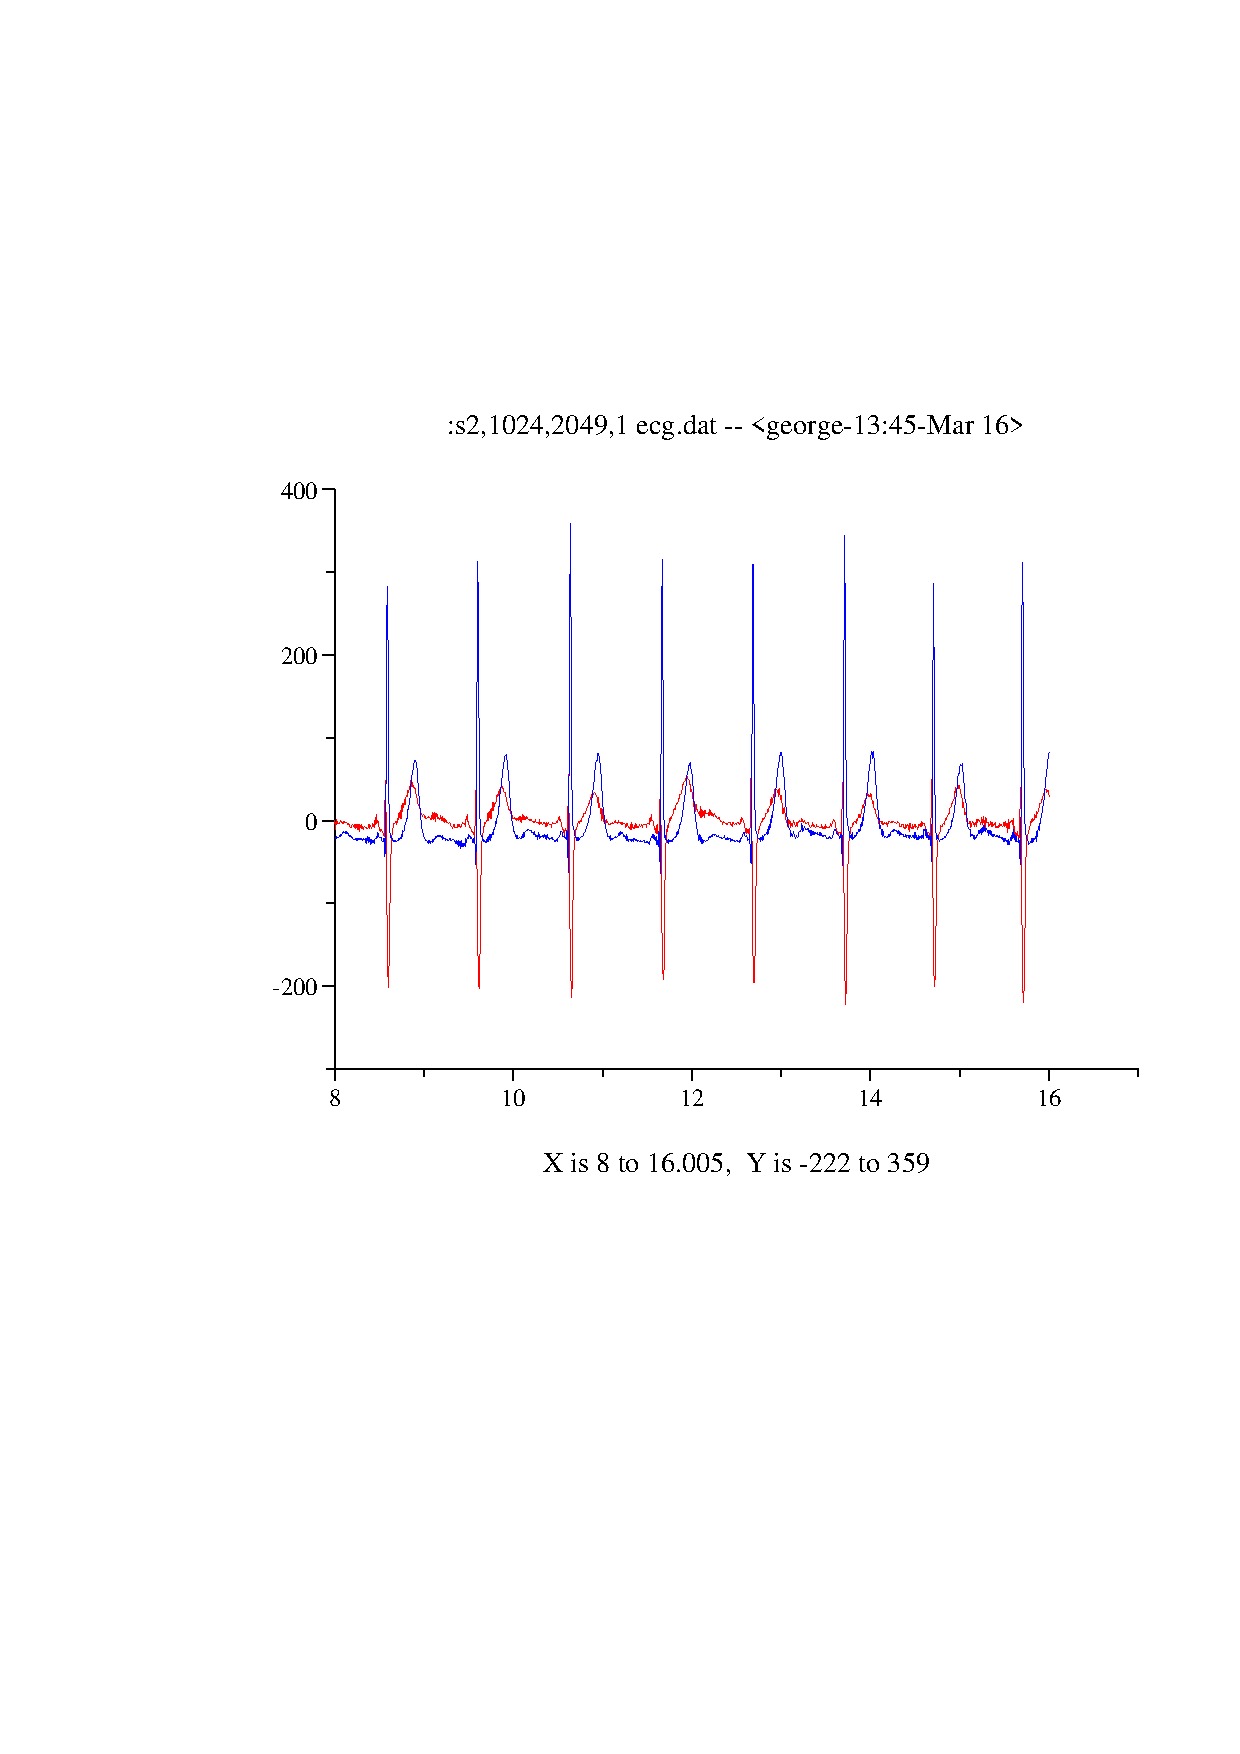
\epsfig{file=ecg,height=10cm}}
\caption[Example with data specification]{Produced using the command:
\label{fig:ecg}}
\begin{center}
\begin{boxedverbatim}
plt :s2,1024,2049,1 ecg.dat \
    -cz 8 .00781 -F"p 0,1n(Cred) 0,2n(Cblue)"
\end{boxedverbatim}
\end{center}
\end{center}
\end{figure}

\section{Format files}

\index{f@{\tt -f} (format file) option}%
As noted earlier, {\tt plt}'s command-line options can also be collected
into {\em format files}, which are read by {\tt plt} if named following
the {\tt -f} option.  The names of format files, as for data files, are
completely arbitrary (in this book, format files have the suffix
{\tt .format}, but this is only for clarity).

Format files are text files.  Like data files, they may contain empty
lines, and any line beginning with '{\tt \#}' is taken to be a comment and
is ignored.

The active ingredients in format files are {\tt plt} options and their
arguments.  In a format file, you must omit the initial hyphen ('{\tt -}')
from each option named.  See chapter~\ref{sec:ax1} for examples of figures
made using command-line arguments with hyphenated options, and using a
format file containing unhyphenated options.

\section{String arrays \label{sec:string-arrays}}

\index{string array}%
\index{text string array}%
\index{fontgroup string array}%
In chapter~\ref{sec:plotting-data}, you will encounter {\tt plt} options that
make use of yet another type of input, namely arrays of strings.  String arrays
can be supplied to {\tt plt} using the {\tt -fs}, {\tt -ts}, and {\tt -tf}
options.  These options take arguments as follows:

\index{fs@{\tt -fs} (define fontgroup string array) option}%
\index{ts@{\tt -ts} (define text string array) option}%
\index{tf@{\tt -tf} (read text string array from file) option}%
\begin{quote}
{\tt -fs "}{$string_{0} \ \  string_{1} \ \  ...$}{\tt "}\\
{\tt -ts "}{$string_{0} \ \  string_{1} \ \  ...$}{\tt "} {\em tbc}\\
{\tt -tf} {\em file} {\em tbc}
\end{quote}

The string argument of {\tt -fs} and {\tt -ts} is treated as an array of
strings (words) separated by white space.  The {\em file} argument of {\tt -tf}
is the name of a file that contains an array of strings separated by newlines
(the strings may include spaces or tabs in this case).  The {\tt -fs} option
defines the {\em fontgroup string array}; the {\tt -ts} and {\tt -tf} options
define the {\em text string array}.  In each case, strings within a string
array are referred to by their index numbers, and (as for the column numbers in
the data file) the index number of the first string in a string array is 0, not
1.

\index{text box coordinates}%
Entries in the text string array can be plotted in the same manner as data
points, by using other options described in chapter~\ref{sec:plotting-data},
together with a data file that specifies the data coordinates and the index
numbers of the strings within the text string array.  The {\em tbc} argument of
{\tt -tf} and {\tt -ts} is optional; if provided, it specifies a {\em text box
coordinate} used to determine how the strings are placed relative to the
coordinates specified by the data file (see chapter~\ref{sec:coord-systems}).
If {\em tbc} is omitted, {\tt plt} centers the strings on the specified
coordinates.

\index{color}%
\index{font}%
\index{line style}%
The fontgroup string array associated with {\tt -fs} has a different purpose;
using the appropriate options, these strings can be used to set the font, line
style (solid, dotted, etc.), or plotting color.  Examples of the use of these
options appear in chapter~\ref{sec:plotting-data}.

\chapter{Coordinate Systems \label{sec:coord-systems}}

Using appropriate {\tt plt} options, you can place labels anywhere in
a plot, and you can place plots anywhere on a page.  These {\tt plt}
options use four coordinate systems to specify position.

\index{xa@{\tt -xa} (set up x axis) option}%
\index{ya@{\tt -ya} (set up y axis) option}%
\index{X@{\tt -X} (set x axis limits) option}%
\index{Y@{\tt -Y} (set y axis limits) option}%
\index{data coordinates}%
First is the {\em data coordinate system}: the coordinates defined by your
plot's axes.  The ranges of the data coordinates depend on the ranges of $x$
and $y$ values, or on the ranges you specify using the {\tt -xa} and {\tt -ya}
(or {\tt -X} and {\tt -Y}) options.  The lower left corner of the data
coordinate system is $(x_{min},y_{min})$, and the upper right corner is
$(x_{max},y_{max})$.

\index{window coordinates}%
Second is the {\em window coordinate system}.  Window coordinates, $(xw,yw)$,
always range from $(0,0)$ to $(1,1)$.  The window coordinates $(0,0)$
correspond to the data coordinates $(x_{min},y_{min})$, and the window
coordinates $(1,1)$ map to the data coordinates $(x_{max},y_{max})$.

\index{X Window System}%
\index{PostScript}%
\index{page coordinates}%
\index{bounding box}%
Third is the {\em page coordinate system}.  Page coordinates, $(xp,yp)$, always
range from $(0,0)$, at the lower left corner of the page, to $(1,1)$ at the
upper right corner.  Using the {\tt -W} option described later on, you can
specify a rectangle in page coordinates in which the plot is to be drawn; this
option thus allows you to draw multiple plots in any desired layout on a page.
When you make a screen plot, the ``page'' may be the entire screen, or it may
be an X window.  When you make a printable plot, the ``page'' may be the entire
sheet of paper, or the printable area (generally less than the full sheet), or
it may represent a PostScript bounding box for a plot that can be incorporated
into another document such as this book.

\begin{figure}
\begin{center}
\fcolorbox{blue}{white}{
\epsfig{file=coords,height=10cm}}
\end{center}
\caption{Data, window, and page coordinates \label{fig:coords}}
\end{figure}

Figure~\ref{fig:coords} illustrates the relationships among data, window, and
page coordinates.  Note that it is always possible to refer to data, window, or
page coordinates outside of the ranges of these coordinate systems.  Depending
on the {\tt plt} options you have chosen, and in some cases on the output
device (screen or printer), out-of-bounds elements may or may not appear in the
output.

\index{text box coordinates}%
A fourth coordinate system, called {\em text box coordinates}, is used by {\tt
plt} to allow fine control over the positioning of text on plots.

{\tt plt} places an imaginary {\em text box} around each string it prints.
Descenders (the lower portions of ``g'', ``j'', ``p'', ``q'', ``y'', and ``,'')
fall outside of the box, but each text box includes extra space above the top
of the characters (30\% to 40\% of the basic height of the text) for any
descenders from the line above.  Text box coordinates are symbolic and discrete
rather than numeric and continuous.  Each text box has twelve points defined as
shown in figure~\ref{fig:example8}.  Thus point {\tt CT} is at the center of
the top side of the text box, {\tt RB} is the lower right corner, etc.

When you tell {\tt plt} to print a string at $(x,y)$, {\tt plt} usually places
text box point {\tt CC} at $(x,y)$, thus centering the string on $(x,y)$.  By
naming the appropriate text box point as an argument to any of the options
described in chapter~\ref{sec:labelling}, {\em Labelling Your Plot}, you can
choose instead to place any of the four corners, the center of any side,
or any of the other defined points of the text box at $(x,y)$.

\begin{figure}
\begin{center}
\fcolorbox{blue}{white}{
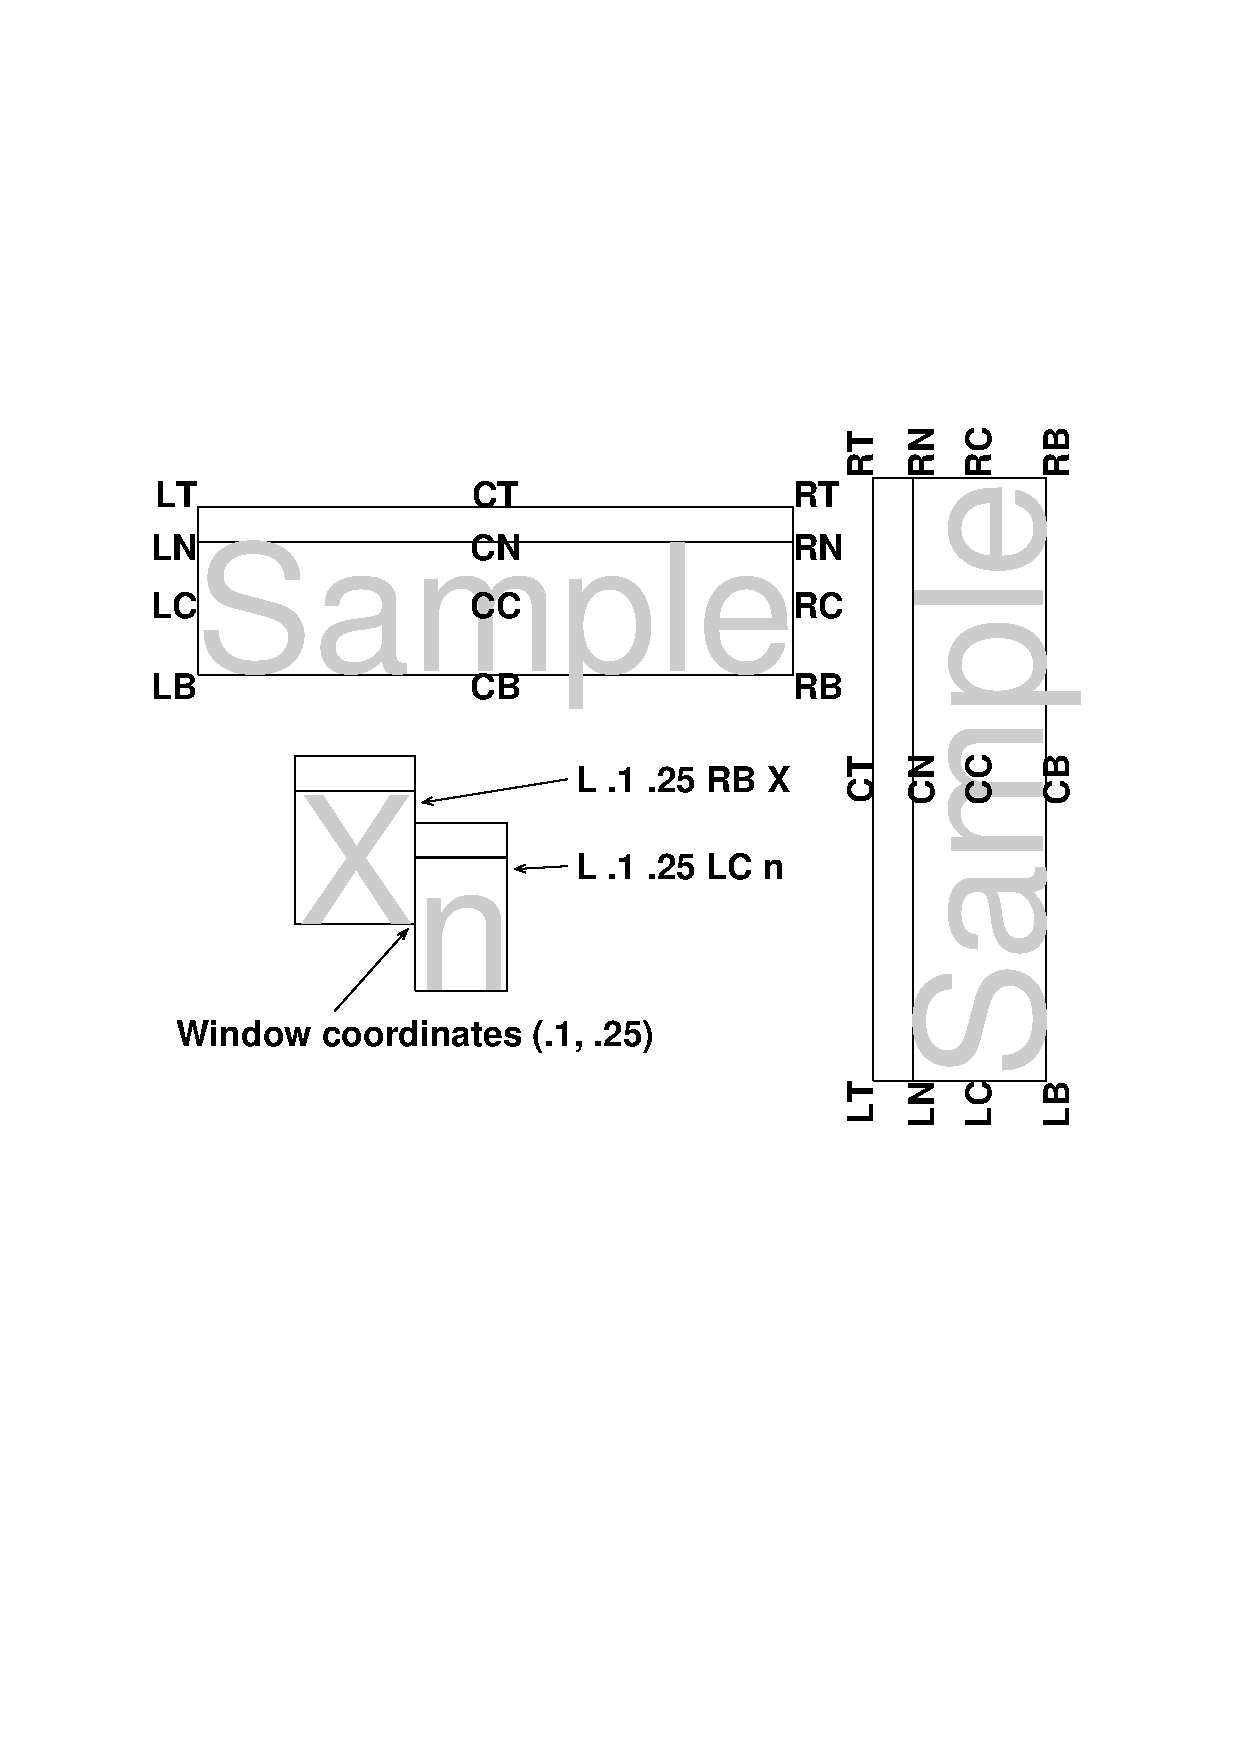
\epsfig{file=figure8,height=10cm}}
\end{center}
\index{subscripts}%
\caption[Text box coordinates]{Text box coordinates. \label{fig:example8} Note
that text box coordinates are always oriented left-right and top-bottom with
respect to the text, and not necessarily with respect to the page.  At lower
left is an example of how to form subscripts using {\tt plt}'s {\tt -L}
option (see chapter~\ref{sec:labelling}).  As shown, the right bottom ({\tt
RB}) point of the {\tt X} and the left center ({\tt LC}) of the subscript {\tt
n} are both placed at the same window coordinates (.1,.25) to achieve the
desired alignment.}
\end{figure}

\chapter{Titles and Axes \label{sec:ax1}}

\index{t@{\tt -t} (plot title) option}%
\index{x@{\tt -x} (x axis title) option}%
\index{y@{\tt -y} (y axis title) option}%
By now you should know how to make a simple plot of data as in the
previous examples.  You are now ready to label your plot.  Using the
{\tt -x} and {\tt -y} options, you can label the x and y axes
respectively.  Using the {\tt -t} option, you can give your plot a
title.  Figure~\ref{fig:example2} demonstrates the use of these options.

\begin{center}
\begin{boxedverbatim}
plt example1.data 0 2  -t "Time vs Amp" \
    -x "time in seconds" -y "amplitude in cm"
\end{boxedverbatim}
\end{center}

\index{column-number@{\em column-number}}%
Note that the data file name and the column numbers should immediately
follow ``{\tt plt}''.

\begin{figure}[h]
\begin{center}
\fcolorbox{blue}{white}{
\epsfig{file=figure2,height=10cm}}
\end{center}
\caption[Generating title and axis labels]{Produced using the command:
\label{fig:example2}}
\begin{center}
\begin{boxedverbatim}
plt example1.data 0 2  -t "Time vs Amp" \
    -x "time in seconds" -y "amplitude in cm"
\end{boxedverbatim}
\end{center}
\end{figure}

\index{xa@{\tt -xa} (set up x axis) option}%
\index{ya@{\tt -ya} (set up y axis) option}%
\index{X@{\tt -X} (set x axis limits) option}%
\index{Y@{\tt -Y} (set y axis limits) option}%
With the {\tt -xa} (x axis) and {\tt -ya} (y axis) options, you can
specify {\em min} and {\em max} (the endpoints of your axes), {\em
tick} (how often you want tick marks to appear), {\em fmt} (the format
in which to print the numbers, e.g., \%.3f, \%.2e), {\em tskip} (how
often to skip when labelling the ticks, and {\em cross} (where you want
the axis you are specifying to cross the other axis, in units of the
other axis).  If you do not need to change the default ticks and axis
crossing points, the {\tt -X} and {\tt -Y} options accept
axis endpoint arguments only.  These options take their arguments as
follows:

\begin{quote}
{\tt -xa} \emph{xmin xmax tick fmt tskip ycross}\\
{\tt -ya} \emph{ymin ymax tick fmt tskip xcross}\\
\\
{\tt -X} \emph{xmin xmax}\\
{\tt -Y} \emph{xmin xmax}
\end{quote}

\index{f@{\tt -f} (format file) option}%
\index{xa@{\tt -xa} (set up x axis) option}%
\index{ya@{\tt -ya} (set up y axis) option}%
Figure~\ref{fig:example3}, on page~\pageref{fig:example3},
demonstrates how {\tt -xa} and {\tt -ya} are used, and also the use of
the {\tt -f} option with a format file.  The format file, named {\tt
example3.format}, looks like this:

\begin{center}
\begin{boxedverbatim}
t Time vs Amp
x time in seconds
y amplitude in cm
xa 0 5 .5 - 2 0
ya 0 5 .5 - 2 0
\end{boxedverbatim}
\end{center}

As for the data file, the name of the format file, including the
suffix if any, is completely arbitrary.  Note that each option within
the format file (in this example, {\tt t}, {\tt x}, {\tt y}, {\tt xa},
and {\tt ya}) must be given without an initial ``{\tt -}'', but that a
``{\tt -}'' in place of an option argument will cause {\tt plt} to
choose its own ``suitable value'' for that argument.  Either a number
based on the size of the plot and data limits will be chosen, or {\tt
plt} will use a default value in place of the ``{\tt -}'' argument.

\begin{figure}[h]
\begin{center}
\fcolorbox{blue}{white}{
\epsfig{file=figure3,height=10cm}}
\end{center}
\caption[Using a format file]{Produced using the command: \label{fig:example3}}
\begin{center}
\begin{boxedverbatim}
plt example1.data 0 2 -f example3.format
\end{boxedverbatim}
\end{center}
\end{figure}

{\tt plt} offers a large number of options that give you control over
virtually every aspect of how axes are drawn and labelled;  these are
described in chapter~\ref{sec:ax2}, beginning on page~\pageref{sec:ax2}.

\section{``Quickplot'' mode \label{sec:quickplot}}

\index{quickplot mode}%
In normal operation, {\tt plt} performs two passes over its input data.  During
the first pass, it reads the data from a file or from its standard input,
allocates memory sufficient to keep the data to be plotted, and determines
suitable axis ranges; during the second pass, {\tt plt} renders the plot.  When
making a screen plot, the intermediate steps are not visible; for efficiency,
the {\tt plt} window is not (re)drawn until the entire image has been prepared
in memory.

\index{xa@{\tt -xa} (set up x axis) option}%
\index{ya@{\tt -ya} (set up y axis) option}%
\index{X@{\tt -X} (set x axis limits) option}%
\index{Y@{\tt -Y} (set y axis limits) option}%
\index{pipe}%
\index{GNU/Linux}%
\index{Linux}%
\index{Mac OS X}%
\index{Unix}%
If, however, you specify both x and y axis ranges using any of the {\tt -xa},
{\tt -ya}, {\tt -X}, and {\tt -Y} options described above, {\em and} if you are
making only one plot (i.e., not using any of the methods described in
chapter~\ref{sec:multiplots} to plot multiple data sets on a single set of
axes), then {\tt plt} runs in {\em quickplot} mode.  In quickplot mode, the
data are read and plotted immediately without buffering, so that for large data
sets the memory requirements and the time needed to render the plot are
significantly reduced.  Quickplot mode allows you to plot data sets that
are larger than the total amount of available memory.  Furthermore, under Unix,
GNU/Linux, and Mac OS X, quickplot mode permits progressive display of
screen plots, so that you do not need to wait for {\tt plt} to read an
entire multi-megabyte input file before seeing any output.  If the data are
provided by a pipe from another process, {\tt plt} can render them in real
time (depending on your hardware speed, at rates up to 50 frames per second,
or even faster if you change the symbol {\tt QPFREQ} in {\tt xw.c} and
recompile {\tt plt}; see appendix~\ref{sec:distribution}).

Figure~\ref{fig:henon} illustrates the final state of a plot of 25,000 points
from a H\'{e}non series.  The command used to generate the figure was:

\begin{center}
\begin{boxedverbatim}
henon | plt % -p s. -X -1.5 1.5 -Y -.5 .5 -t "Henon Attractor"
\end{boxedverbatim}
\end{center}

\noindent
You can see quickplot mode in action if you compile {\tt henon} from the
source (a file named {\tt henon.c}, provided in the {\tt doc} directory of
the {\tt plt} distribution) and then run the command above.  Delays are
included in {\tt henon.c} so that you will be able to see what happens
even with a fast CPU.  Over a period of several seconds, the picture of the
H\'{e}non attractor emerges.

\begin{figure}[h]
\begin{center}
\fcolorbox{blue}{white}{
\epsfig{file=henon,height=8cm}}
\end{center}
\caption{H\'{e}non attractor, produced in {\em quickplot}
mode\label{fig:henon}}.
\end{figure}

\chapter{Plotting Data \label{sec:plotting-data}}

\index{p@{\tt -p} (plotstyle) option}%
Most of the previous examples have illustrated how two columns of data can be
plotted as a connected set of line segments.  This is {\tt plt}'s
default style for plotting data, but many other styles are supported
using the {\tt -p} option to choose a {\em plotstyle}.  For example, data can
be plotted using points, characters, strings, or symbols (scatter
plots);  with error bars;  or using lines of various widths, grey levels,
colors, or patterns (solid, dotted, etc.).

\index{color}%
\index{font}%
\index{line width}%
\index{width of line}%
\index{line style}%
To specify a plotstyle, we can use the {\tt -p} option, followed by
sub-options that control how the points are plotted.  Each sub-option
can also have an optional argument following it.  This argument can
change the font, point size, color, gray scale, line width, or line
style (solid, dotted, dashed, etc.)  of the current plot.  (If you want
to use those control options that enable you to make font changes, you
will need to read and understand chapter~\ref{sec:font-groups}, {\em
Colors, Line Styles, and Fonts}, beginning on
page~\pageref{sec:font-groups}.)

\index{column-number@{\em column-number}}%
Each plotstyle ``takes'' (consumes) one or more data columns.  If you
use more than one plotstyle, you must include enough data column
numbers for all of the plotstyles in the {\tt plt} command line.  Note
that you may repeat data column numbers if necessary to satisfy the
requirements of the plotstyles you select;  see the examples below to
see how this can be done.

If you have not used {\tt plt} previously, it is probably a bad idea
to read through this chapter from beginning to end, because the usage
of the plotstyles (especially the first one listed below, {\tt c}) is
mind-bogglingly convoluted.  A better strategy is to begin by studying
the examples in this chapter; find one or more that illustrate
features you would like to use in your own plots, then see which
plotstyles were used to obtain these features.

\newpage
The sub-options to {\tt -p} are:

\index{p@{\tt -p} (plotstyle) option!c@{\tt c} (control) suboption}%
\begin{description}
\item[{\tt c}]
Takes three data columns ($x$, $y$, and $c$).
Each $c$ value tells {\tt plt} what to do with the corresponding $x$
and $y$ values.  The values for $c$ can be:
\end{description}
\begin{center}
\begin{tabular}{p{2.5cm}p{8.5cm}}
{\tt 0} & {continue (draw) path to $(x,y)$} \\
{\tt 1} & {move to $(x,y)$ without drawing (i.e., with the ``pen''
up), then put the pen down (begin a new path)} \\
{\tt 2} & {put a dot at $(x,y)$} \\
{\tt 3} & {put a small box at $(x,y)$} \\
{\tt 9} & {paint the path (usually done as the default when a new path is begun
without specifying what to do with the old one)} \\
{\tt 10} & {continue to $(x,y)$, close path and fill the inside with grey level
specified by the argument to the {\tt c} sub-option} \\
{\tt 11} & {continue to $(x,y)$, close path and fill the inside with grey level
specified by the argument to the {\tt c} sub-option; then draw a black
border} \\
{{\tt 12} -- {\tt 13}} & {continue to $(x,y)$, close path and
fill the inside with grey level specified by $c-12$ (12.0~=~black,
13.0~=~white)} \\
{{\tt 14} -- {\tt 15}} & {continue to $(x,y)$, close path and fill the
inside with grey level specified by $c-14$ (14.0 = black, 15.0 = white);
then draw a black border} \\
{\tt 20} & {(requires {\tt -fs} option, see section~\ref{sec:string-arrays},
{\em String arrays}, page~\pageref{sec:string-arrays}) change font to that
specified by string number $x$ from the {\tt -fs} string array} \\
{\tt 21} & {change point size to $x$} \\
{\tt 22} & {change line width to $x$} \\
{\tt 23} & {(requires {\tt -fs} option, see section~\ref{sec:string-arrays})
change line style to that specified by string number $x$ from the {\tt -fs}
string array; legal line styles are ``{\tt solid}'', ``{\tt dotted}'',
``{\tt shortdashed}'', ``{\tt dotdashed}'', and ``{\tt longdashed}''.  Note
that $y$ is ignored (see figure~\ref{fig:example4}).} \\
{\tt 24} & {change grey level to $x$ (0 = black, 1 = white); $y$ is ignored.}\\
{\tt 25} & {(requires {\tt -fs} option, see section~\ref{sec:string-arrays})
change color to that specified by string number $x$ from the fontgroup
string array (see appendix~\ref{sec:color-names} for details on how to specify
colors by name; also, note that $y$ is ignored)} \\
{{\tt 30} -- {\tt 39}} & {put symbol number $c-30$ at $(x,y)$ (see
figure~\ref{fig:symbols})} \\
{\tt 100, 101, ...} & {(requires {\tt -tf} or {\tt -ts} option, see
section~\ref{sec:string-arrays}) put string number {\em control-100} from the
text string array at $(x,y)$}
\end{tabular}
\end{center}

\begin{figure}
\begin{center}
\begin{tabular}{p{10cm}p{1.5cm}}
\fcolorbox{blue}{white}{
\epsfig{file=figure4,height=8cm}} &
{\vspace{-8cm}
{\em Data}
\vspace*{3mm}

\begin{boxedverbatim}
0 0 0
3 3 0
1 7 23
4 4 0
7 7 0
2 6 23
8 8 0
10 10 0
\end{boxedverbatim}
}
\end{tabular}
\end{center}
\caption[Changing line styles]{Produced using the command:
\label{fig:example4}}
\begin{center}
\begin{boxedverbatim}
plt example4.data 0 1 2 -F"\
    fs helvetica longdashed dotted\
    p c"
\end{boxedverbatim}
\end{center}
The two lines in the data file (at right, above) in which the third column
($c$) is 23 change the line styles to string $x$ (the number specified in the
first column) from the fontgroup string array.  The fontgroup string array is
defined in the command line above (string 0 is ``{\tt helvetica}'', not used in
this example; string 1 is ``{\tt longdashed''}; and string 2 is ``{\tt
dotted}'').  Thus when {\tt plt} reads {\tt 1 7 23}, the line style changes
from the default (``{\tt solid}'') to the style specified by string 1 (``{tt
longdashed}''; the 7 is ignored), and when it reads {\tt 2 6 23}, the line
style becomes ``{\tt dotted}'' (and the 6 is similarly ignored).

\hspace{2em}The line segments are not connected, because each non-zero $c$
value causes the previous segment to be drawn, and a new segment begins at the
next $(x,y)$ pair.  If you wish to connect line segments in a plot such as
this, the input file must provide the segments' common endpoints twice, once
each before and after the line that changes {\tt plt}'s line style.
\end{figure}
\begin{figure}
\begin{center}
\fcolorbox{blue}{white}{
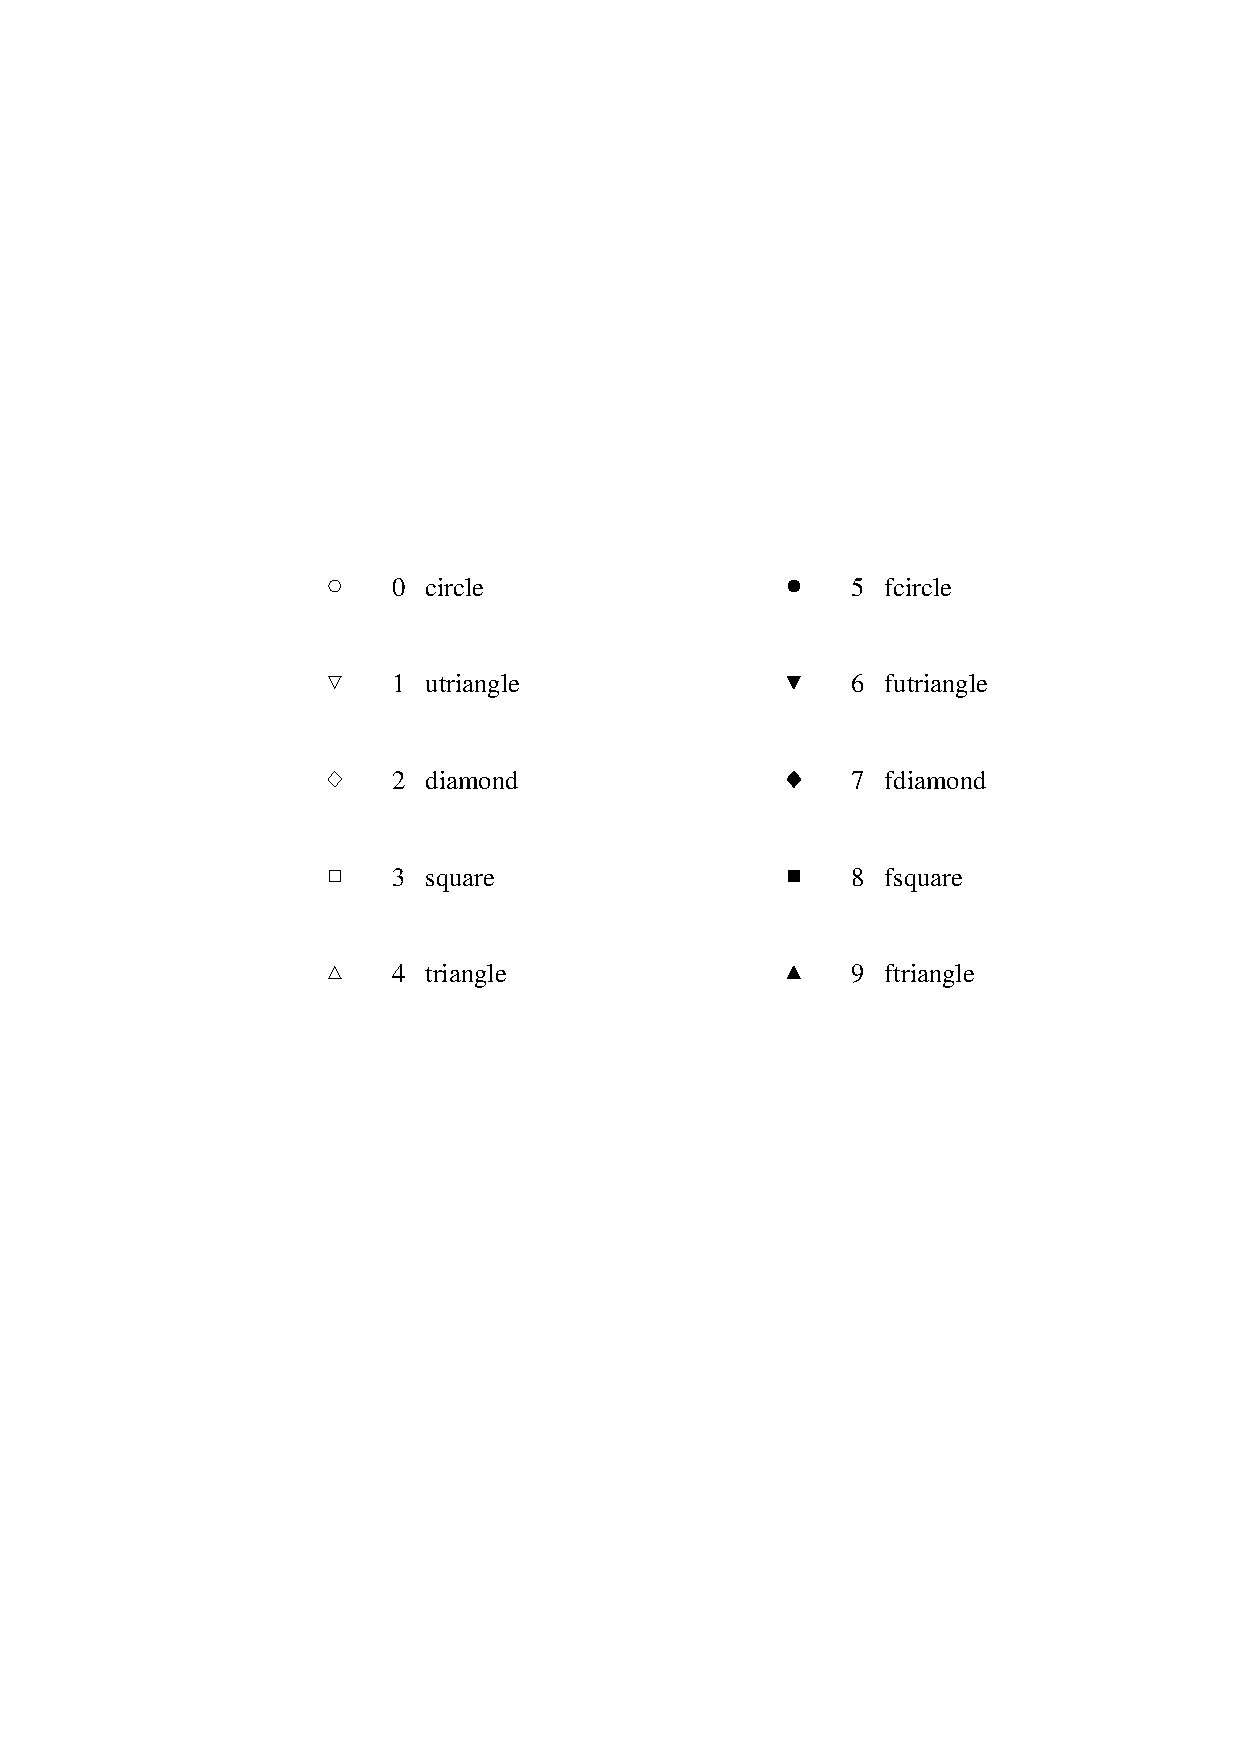
\epsfig{file=symbols,height=10cm}}
\end{center}
\caption[Open and filled plot symbols]{The ten symbols \label{fig:symbols} that
can be plotted using plotstyles {\tt c} (suboptions 30 through 39), {\tt E},
and {\tt S}.  Numeric (0-9) and mnemonic (``circle'', ``square'', etc.) names
appear to the right of each symbol; either form may be used when specifying a
symbol to be used with plotstyles {\tt E} or {\tt S}.  The open symbols (0
through 4) have opaque centers; these are particularly recommended for
relatively dense scatter plots because it is still possible to distinguish and
count individual data points even when the symbols partially overlap.  The size
of the symbols is determined by the current font's point size (see the
description of the {\tt -sf} option in chapter~\ref{sec:font-groups}), {\em
Colors, Line Styles, and Fonts}, beginning on page~\pageref{sec:font-groups}.}
\end{figure}

\begin{description}
\item[{\tt C}]
\index{p@{\tt -p} (plotstyle) option!C@{\tt C} (connect) suboption}%
\index{color}%
Takes two columns, $x$ and $y$, assumed to be the vertices of a polygon.
The polygon is drawn by connecting consecutive vertices and by
connecting the last vertex to the first, and then it is filled in the
current color (default: black).  Nonconvex and self-intersecting
polygons are filled properly.
See figure~\ref{fig:style-C}, page~\pageref{fig:style-C}.

\item[{\tt e+$c$}]
\index{p@{\tt -p} (plotstyle) option!e@{\tt e} (error bars) suboption}%
Takes three columns ($x$, $y$, and $e$).  This sub-option
makes a scatter plot, like {\tt s} (see below), but including error bars.  Each
$e$ value tells {\tt plt} the size of the error associated with the
corresponding $x$ and $y$.  When using the {\tt e} sub-option, you may specify
the character (default: ``{\tt *}'') to use when plotting $(x,y)$, and you must
indicate if you wish to plot the top, bottom, or both halves of the error bars,
as follows:
\item[{\tt e-$c$}]
\vspace{-24.5mm}
\item[{\tt e:$c$}]
\vspace{-3.5mm}
~
\begin{description}
\item[{\tt e+$c$}]
\vspace{13mm}
plot $(x,y)$ as ``$c$'', with top half of error bars only
\item[{\tt e-$c$}]
plot $(x,y)$ as ``$c$'', with bottom half of error bars only
\item[{\tt e:$c$}]
plot $(x,y)$ as ``$c$'', with both top and bottom error bars;
the ``:'' may be omitted unless $c$ is either ``{\tt +}'' or
``{\tt -}''
\end{description}

\item[{\tt E+$n$}]
\index{p@{\tt -p} (plotstyle) option!E@{\tt E} (error bars with symbols) suboption}%
Takes three columns ($x$, $y$, and $e$).
Exactly like its counterpart, {\tt e}, except that this sub-option
allows you to plot a specified symbol (identified by a symbol number $n$
between 0 and 9 inclusive) instead of a character.
\item[{\tt E-$n$}]
\vspace{-12mm}
\item[{\tt E:$n$}]
\vspace{-3.5mm}
~

\item[{\tt f}]
\index{p@{\tt -p} (plotstyle) option!f@{\tt f} (fill area) suboption}%
\index{color}%
\vspace{1mm}
Takes three columns ($x$, $y_0$, and $y_1$) and fills the area defined
by the normal plots of $(x,y_0)$ and $(x,y_1)$ in the current color
(default: black).
See figure~\ref{fig:style-f}, page~\pageref{fig:style-f}.

\item[{\tt i}]
\index{p@{\tt -p} (plotstyle) option!i@{\tt i} (impulse response) suboption}%
Takes two columns, $x$ and $y$.  The $(x,y)$ pairs are
plotted in impulse response form.
See figure~\ref{fig:style-i}, page~\pageref{fig:style-i}.

\item[{\tt l}]
\index{p@{\tt -p} (plotstyle) option!l@{\tt l} (line segments) suboption}%
Takes four columns, $x_{0}$, $y_{0}$, $x_{1}$, and $y_{1}$.  The line
segments with endpoints $(x_{0},y_{0})$ and $(x_{1},y_{1})$ are plotted.
See figure~\ref{fig:style-l}, page~\pageref{fig:style-l}.

\item[{\tt m}]
\index{p@{\tt -p} (plotstyle) option!m@{\tt m} (single-column normal plot) suboption}%
\index{column-number@{\em column-number}}%
Takes one column ($y$).  The $x$ values are always taken from column 0
of the input.  The output is a normal plot of $(x,y)$ pairs.  (If you supply
only one data column number to {\tt plt} and do not specify a
plotstyle, this is the type of plot you will obtain by default.)
See figure~\ref{fig:style-m}, page~\pageref{fig:style-m}.

\item[{\tt n}]
\index{p@{\tt -p} (plotstyle) option!n@{\tt n} (two-column normal plot) suboption}%
\index{column-number@{\em column-number}}%
Takes two columns, $x$ and $y$.  The output is a normal plot
of $(x,y)$ pairs.  (If you supply two data column numbers to {\tt
plt} and do not specify a plotstyle, this is the type of plot you will
obtain by default.)
See figure~\ref{fig:style-n}, page~\pageref{fig:style-n}.

\item[{\tt N}]
\index{p@{\tt -p} (plotstyle) option!N@{\tt N} (normal plot filled) suboption}%
\index{color}%
Takes two columns, $x$ and $y$.  The area bounded by the normal plot of
the $(x,y)$ pairs and the x axis is filled with the current color (default:
black).
See figure~\ref{fig:style-N}, page~\pageref{fig:style-N}.

\item[{\tt o}]
\index{p@{\tt -p} (plotstyle) option!o@{\tt o} (outline) suboption}%
\index{color}%
Takes three columns ($x$, $y_0$, and $y_1$) and outlines the area defined
by the normal plots of $(x,y_0)$ and $(x,y_1)$ in the current color (default:
black).
See figure~\ref{fig:style-o}, page~\pageref{fig:style-o}.

\item[{\tt O}]
\index{p@{\tt -p} (plotstyle) option!O@{\tt O} (outline and fill) suboption}%
\index{color}%
Takes three columns ($x$, $y_0$, and $y_1$), outlines the area defined
by the normal plots of $(x,y_0)$ and $(x,y_1)$ in black, and fills this
area in the current color (default: black).
See figure~\ref{fig:style-O}, page~\pageref{fig:style-O}.

\item[{\tt s$c$}]
\index{p@{\tt -p} (plotstyle) option!s@{\tt s} (scatter plot) suboption}%
Takes two columns, $x$ and $y$.  The output is a scatter plot of $(x,y)$
pairs, where each pair is plotted using the character specified by $c$
(a character suffixed to the plotstyle name, {\tt s}).
See figure~\ref{fig:style-sO}, page~\pageref{fig:style-sO}.

\item[{\tt S$n$}]
\index{p@{\tt -p} (plotstyle) option!s@{\tt S} (scatter plot using symbols) suboption}%
Takes two columns, $x$ and $y$.  Exactly like its counterpart, {\tt
s}, except that this plotstyle allows you to plot a specified symbol
(identified by a symbol number $n$ between 0 and 9 inclusive), instead
of a character.
See figure~\ref{fig:style-Sfdiamond}, page~\pageref{fig:style-Sfdiamond}.

\item[{\tt t}]
\index{p@{\tt -p} (plotstyle) option!t@{\tt t} (scatter plot using text strings) suboption}%
\index{text box coordinates}%
Takes three columns, $x$, $y$, and $n$.  
This plotstyle must be used together with the {\tt -tf} or {\tt -ts}
option (see section~\ref{sec:string-arrays}).  The $n$ values specify strings
from the {\tt -tf} or {\tt -ts} string array;  {\tt plt} prints these
at the locations given by the corresponding $(x,y)$ pairs (adjusting the
string positions according to the text box coordinates provided to the
{\tt -tf} or {\tt -ts} option). See figure~\ref{fig:style-t},
page~\pageref{fig:style-t}.
\end{description}

\section{A gallery of plotstyles}

This section contains a series of plots made using many of the plotstyles
described in the previous pages.  Each plot was made using the same data
file, {\tt styles.data}, which contains:

\begin{center}
\begin{boxedverbatim}
0 0 0 0
1 -1 .25 1
2 -2 .5 2
3 1 .25 1
4 4 1 4
5 1 .25 1
6 -2 .5 2
7 -1 .25 1
8 0 0 0
\end{boxedverbatim}
\end{center}

In several of these examples, the data are plotted in 90\% grey, to make clear
how certain plotstyles use the plot color.  {\tt plt} is told to do this by
the ``{\tt (G.90)}'' appended to the plotstyle specification in each case;  see
chapter~\ref{sec:font-groups} for details on using color and grey level
definitions such as these.

\begin{figure}[h]
\begin{center}
\fcolorbox{blue}{white}{
\epsfig{file=style-C,height=6.5cm}}
\end{center}
\caption[Plotstyle C]{Produced using the command:
\label{fig:style-C}}
\begin{center}
\begin{boxedverbatim}
plt styles.data -p "0,1C(G.90)" -t "Plotstyle C"
\end{boxedverbatim}
\end{center}
\end{figure}

\begin{figure}
\begin{center}
\fcolorbox{blue}{white}{
\epsfig{file=style-e+Z,height=6.5cm}}
\end{center}
\caption[Plotstyle e+Z]{Produced using the command:
\label{fig:style-e+Z}}
\begin{center}
\begin{boxedverbatim}
plt styles.data -p 0,1,2e+Z -t "Plotstyle e+Z"
\end{boxedverbatim}
\end{center}
\end{figure}

\begin{figure}
\begin{center}
\fcolorbox{blue}{white}{
\epsfig{file=style-e-X,height=6.5cm}}
\end{center}
\caption[Plotstyle e-X]{Produced using the command:
\label{fig:style-e-X}}
\begin{center}
\begin{boxedverbatim}
plt styles.data -p 0,1,2e-X -t "Plotstyle e-X"
\end{boxedverbatim}
\end{center}
\end{figure}

\begin{figure}
\begin{center}
\fcolorbox{blue}{white}{
\epsfig{file=style-ec+,height=6.5cm}}
\end{center}
\caption[Plotstyle e:+]{Produced using the command:
\label{fig:style-e:+}}
\begin{center}
\begin{boxedverbatim}
plt styles.data -p 0,1,2e:+ -t "Plotstyle e:+"
\end{boxedverbatim}
\end{center}
\end{figure}

\begin{figure}
\begin{center}
\fcolorbox{blue}{white}{
\epsfig{file=style-E+0,height=6.5cm}}
\end{center}
\caption[Plotstyle E+0]{Produced using the command:
\label{fig:style-E+0}}
\begin{center}
\begin{boxedverbatim}
plt styles.data -p 0,1,2E+0 -t "Plotstyle E+0"
\end{boxedverbatim}
\end{center}
\end{figure}

\begin{figure}
\begin{center}
\fcolorbox{blue}{white}{
\epsfig{file=style-E-ftriangle,height=6.5cm}}
\end{center}
\caption[Plotstyle E-ftriangle]{Produced using the command:
\label{fig:style-E-ftriangle}}
\begin{center}
\begin{boxedverbatim}
plt styles.data -p 0,1,2E-ftriangle -t "Plotstyle E-ftriangle"
\end{boxedverbatim}
\end{center}
\end{figure}

\begin{figure}
\begin{center}
\fcolorbox{blue}{white}{
\epsfig{file=style-Ecsquare,height=6.5cm}}
\end{center}
\caption[Plotstyle E:square]{Produced using the command:
\label{fig:style-E:square}}
\begin{center}
\begin{boxedverbatim}
plt styles.data -p 0,1,2E:square -t "Plotstyle E:square"
\end{boxedverbatim}
\end{center}
\end{figure}

\begin{figure}
\begin{center}
\fcolorbox{blue}{white}{
\epsfig{file=style-f,height=6.5cm}}
\end{center}
\caption[Plotstyle f]{Produced using the command:
\label{fig:style-f}}
\begin{center}
\begin{boxedverbatim}
plt styles.data -p "0,1,2f(G.90)" -t "Plotstyle f"
\end{boxedverbatim}
\end{center}
\end{figure}

\begin{figure}
\begin{center}
\fcolorbox{blue}{white}{
\epsfig{file=style-i,height=6.5cm}}
\end{center}
\caption[Plotstyle i]{Produced using the command:
\label{fig:style-i}}
\begin{center}
\begin{boxedverbatim}
plt styles.data -p 0,1i -t "Plotstyle i"
\end{boxedverbatim}
\end{center}
\end{figure}

\begin{figure}
\begin{center}
\fcolorbox{blue}{white}{
\epsfig{file=style-l,height=6.5cm}}
\end{center}
\caption[Plotstyle l]{Produced using the command:
\label{fig:style-l}}
\begin{center}
\begin{boxedverbatim}
plt styles.data -p 0,1,0,3l -t "Plotstyle l"
\end{boxedverbatim}
\end{center}
\end{figure}

\begin{figure}
\begin{center}
\fcolorbox{blue}{white}{
\epsfig{file=style-m,height=6.5cm}}
\end{center}
\caption[Plotstyle m]{Produced using the command:
\label{fig:style-m}}
\begin{center}
\begin{boxedverbatim}
plt styles.data -p 1m -t "Plotstyle m"
\end{boxedverbatim}
\end{center}
\end{figure}

\begin{figure}
\begin{center}
\fcolorbox{blue}{white}{
\epsfig{file=style-n,height=6.5cm}}
\end{center}
\caption[Plotstyle n]{Produced using the command:
\label{fig:style-n}}
\begin{center}
\begin{boxedverbatim}
plt styles.data -p 0,1n -t "Plotstyle n"
\end{boxedverbatim}
\end{center}
\end{figure}

\begin{figure}
\begin{center}
\fcolorbox{blue}{white}{
\epsfig{file=style-N,height=6.5cm}}
\end{center}
\caption[Plotstyle N]{Produced using the command:
\label{fig:style-N}}
\begin{center}
\begin{boxedverbatim}
plt styles.data -p "0,1N(G.90)" -t "Plotstyle N"
\end{boxedverbatim}
\end{center}
\end{figure}

\begin{figure}
\begin{center}
\fcolorbox{blue}{white}{
\epsfig{file=style-o,height=6.5cm}}
\end{center}
\caption[Plotstyle o]{Produced using the command:
\label{fig:style-o}}
\begin{center}
\begin{boxedverbatim}
plt styles.data -p 0,1,2o -t "Plotstyle o"
\end{boxedverbatim}
\end{center}
\end{figure}

\begin{figure}
\begin{center}
\fcolorbox{blue}{white}{
\epsfig{file=style-O,height=6.5cm}}
\end{center}
\caption[Plotstyle O]{Produced using the command:
\label{fig:style-O}}
\begin{center}
\begin{boxedverbatim}
plt styles.data -p "0,1,2O(G.90)" -t "Plotstyle O"
\end{boxedverbatim}
\end{center}
\end{figure}

\begin{figure}
\begin{center}
\fcolorbox{blue}{white}{
\epsfig{file=style-sO,height=6.5cm}}
\end{center}
\caption[Plotstyle sO]{Produced using the command:
\label{fig:style-sO}}
\begin{center}
\begin{boxedverbatim}
plt styles.data -p 0,1sO -t "Plotstyle sO"
\end{boxedverbatim}
\end{center}
\end{figure}

\begin{figure}
\begin{center}
\fcolorbox{blue}{white}{
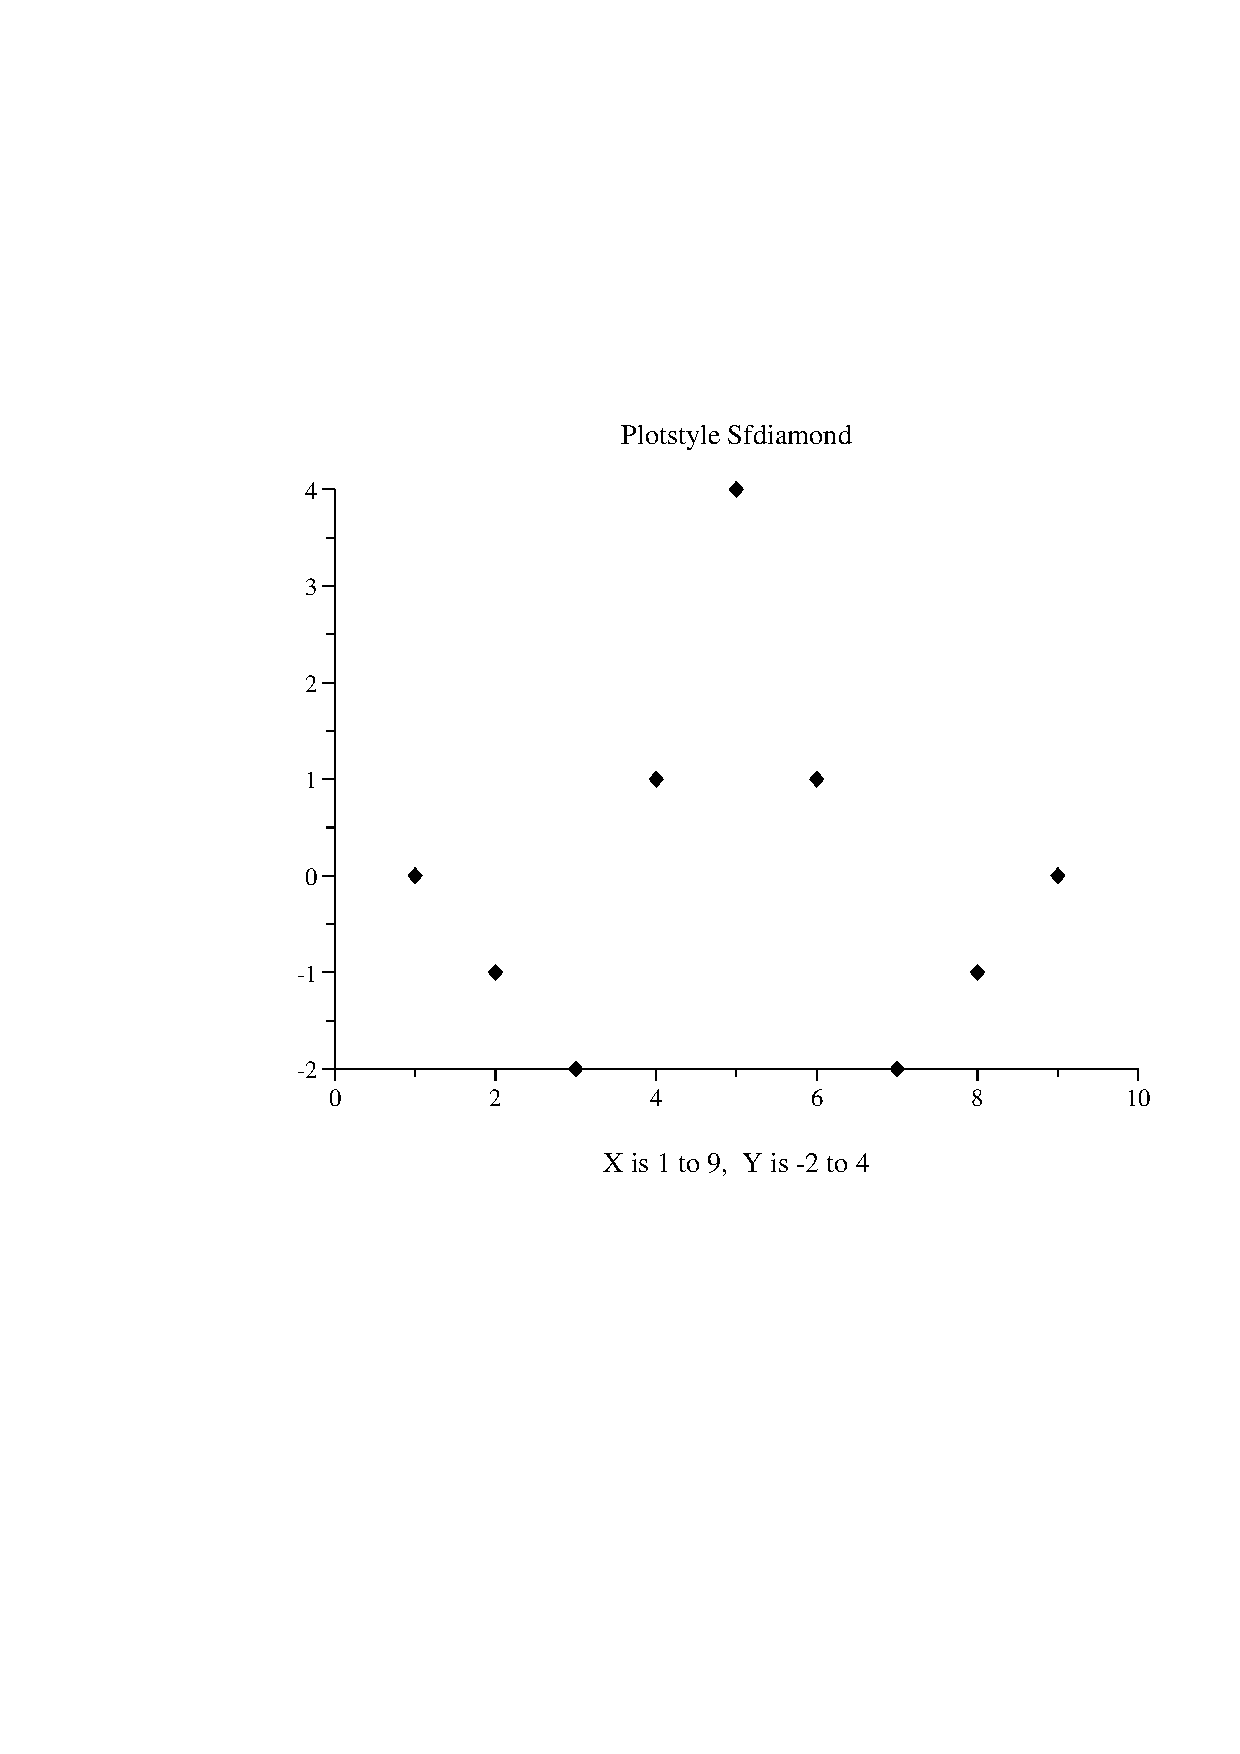
\epsfig{file=style-Sfdiamond,height=6.5cm}}
\end{center}
\caption[Plotstyle Sfdiamond]{Produced using the command:
\label{fig:style-Sfdiamond}}
\begin{center}
\begin{boxedverbatim}
plt styles.data -p 0,1Sfdiamond -t "Plotstyle Sfdiamond"
\end{boxedverbatim}
\end{center}
\end{figure}

\begin{figure}
\begin{center}
\fcolorbox{blue}{white}{
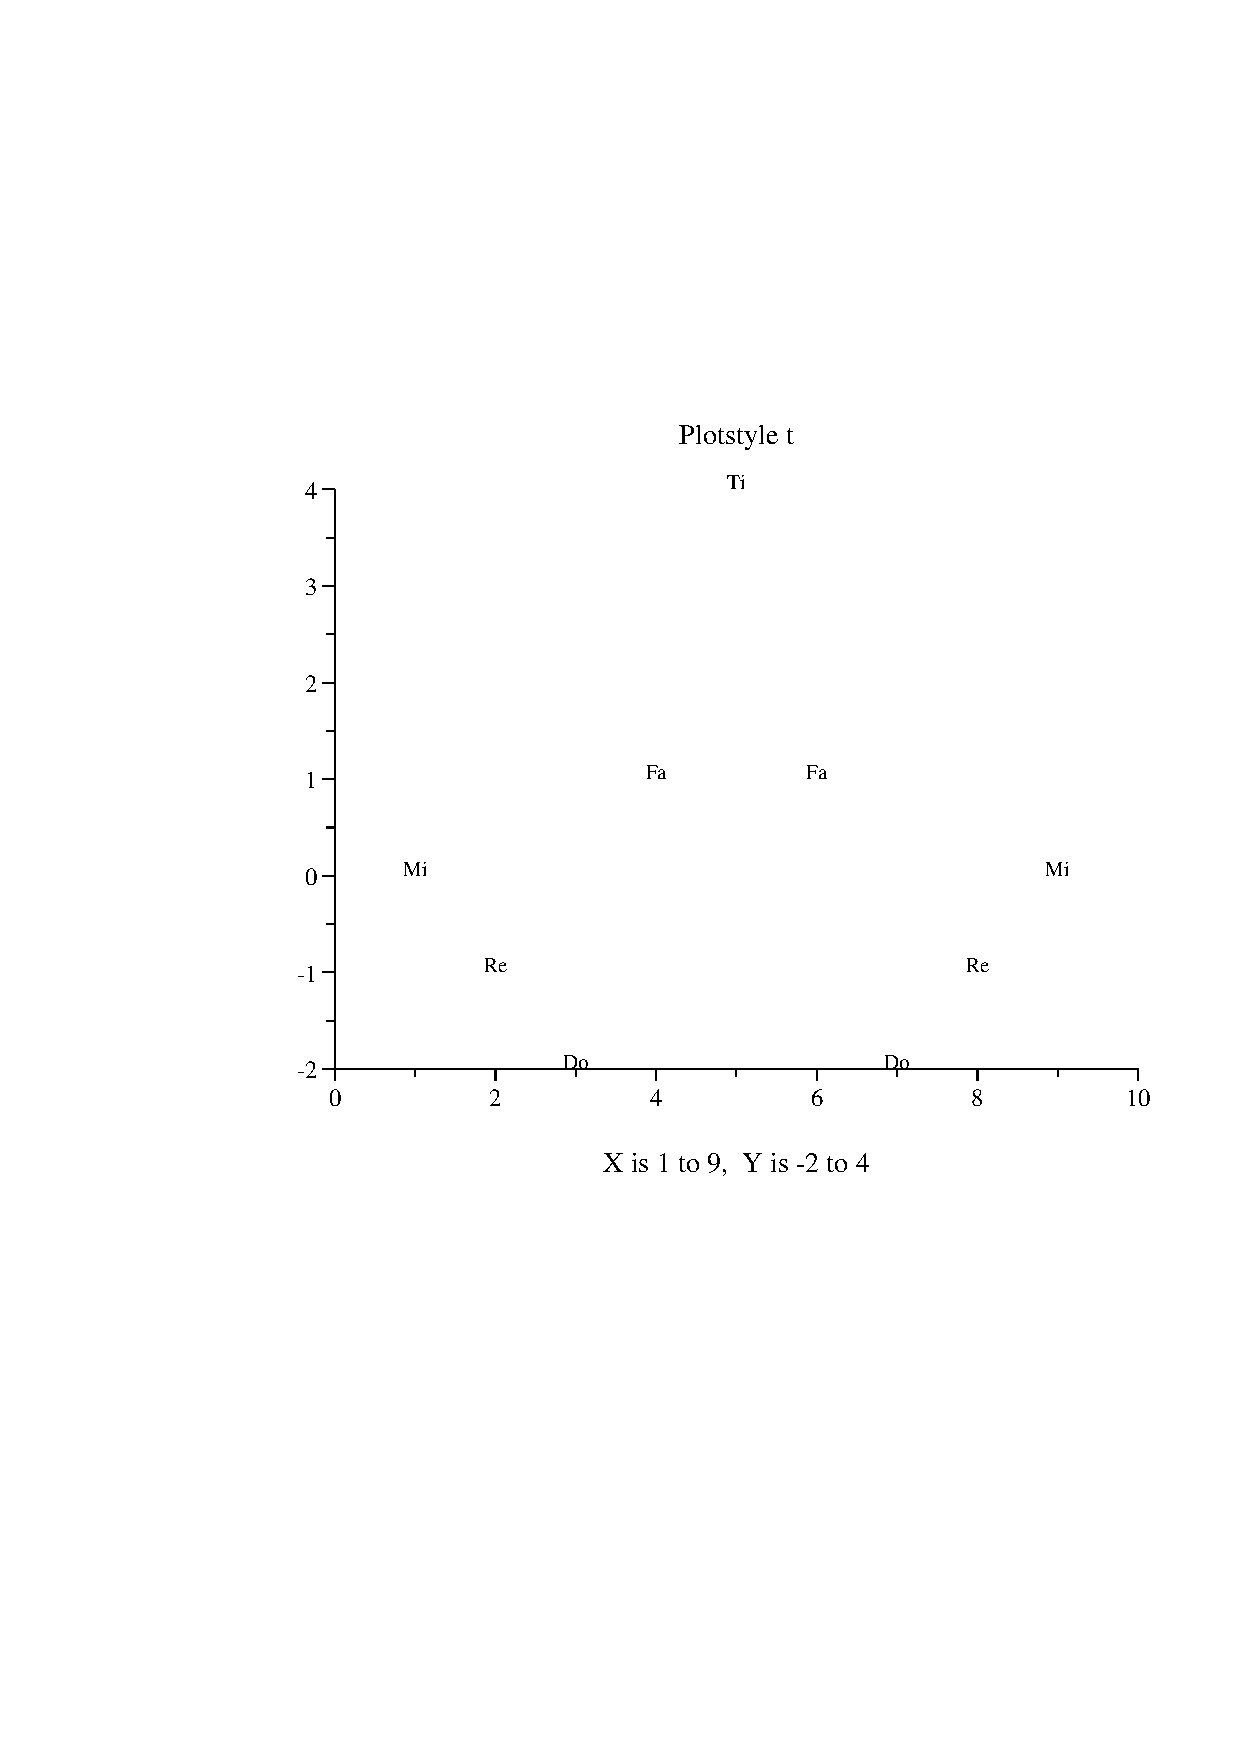
\epsfig{file=style-t,height=6.5cm}}
\end{center}
\caption[Plotstyle t]{Produced using the command:
\label{fig:style-t}}
\begin{center}
\begin{boxedverbatim}
plt styles.data -p 0,1,3t -t "Plotstyle t" \
    -ts "Do Re Mi Fa Sol La Ti" CB
\end{boxedverbatim}
\end{center}
\end{figure}


\chapter{Plotting Two or More Data Sets Together \label{sec:multiplots}}

\index{overlays}%
Until now, most of the plots we have seen show only one data set.
Often, as in figure~\ref{fig:ecg}, on page~\pageref{fig:ecg}, it may be
useful to plot two or more data sets together.
There are several ways to arrange more than one plot on a page or
window.  This chapter shows first how you can overlay plots; how you
can use different plot styles and create legends (or keys) so that
overlaid plots can be distinguished; and finally how you can arrange
plots side-by-side on a page or window.

\section{Plotting multiple data sets on one set of axes \label{sec:overlays}}

{\tt plt} can plot more than one data set on the same set of axes.
There are several ways to overlay plots.

\begin{figure}
\begin{center}
\begin{tabular}{p{10cm}p{1.5cm}}
\fcolorbox{blue}{white}{
\epsfig{file=figure6,height=8cm}} &
{\vspace{-8cm}
{\em Data}
\vspace*{3mm}

\begin{boxedverbatim}
0 0 0 0
1 1 2 3
2 2 4 6
3 3 6 9
4 4 8 12
5 5 10 15
\end{boxedverbatim}
}
\end{tabular}
\end{center}
\caption[Normal and scatter plots]{Produced using the command:
\label{fig:example6}}
\begin{center}
\begin{boxedverbatim}
plt example5.data 0 3 0 2 1 -F"p s+ s* m"
    -x "x axis" -y "y axis" -t "plot of y=x; y=2x and y=3x"
\end{boxedverbatim}
\end{center}
This command produces three traces on the same pair of axes (using
``{\tt +}'' to make a scatter plot of columns 0 and 3, ``{\tt *}'' to
make another scatter plot of columns 0 and 2, and using columns 0 and
1 to make a normal plot).
\end{figure}

\index{p@{\tt -p} (plotstyle) option}%
Figure~\ref{fig:example6} demonstrates the use of the {\tt -p} option to
specify multiple plots in a single invocation of {\tt plt}, using a data
file that includes a column of ordinates for each plot.  The figure can
be produced using any of these commands:

\begin{center}
\begin{boxedverbatim}
plt example5.data 0 3 0 2 1 -F"p s+ s* m"
    -x "x axis" -y "y axis" -t "plot of y=x; y=2x and y=3x"

plt example5.data 0 1 2 3 -F"p 0,3s+ 0,2s* 1m"
    -x "x axis" -y "y axis" -t "plot of y=x; y=2x and y=3x"

plt example5.data % -F"p 0,3s+ 0,2s* 1m"
    -x "x axis" -y "y axis" -t "plot of y=x; y=2x and y=3x"
\end{boxedverbatim}
\end{center}

\index{column-number@{\em column-number}}%
There are several ways of specifying the data columns to be ``taken'' by the
{\tt -p} plotstyles.  In the first command, the data columns are listed (after
the name of the data file) in the order they are taken (the first '{\tt s}'
takes column 0 as $x$ and column 3 as $y$, the second '{\tt s}' takes column 0
as $x$ and column 2 as $y$, and the '{\tt m}' takes column 1 as $y$ and
implicitly takes column 0 as $x$).  In the second command, {\em all} of the
data columns are listed in order after the name of the data file, and each
plotstyle name is prefixed with a comma-separated list of the data columns it
takes.  The third command illustrates how ``{\tt \%}'' can be used as shorthand
for ``all of the data columns, in order''; it is equivalent to the second
command.

\index{fa@{\tt -fa} (save axis setup in file) option}%
\index{o@{\tt -o} (overlay) option}%
If the data sets to be overlaid come from different files, it will be easiest
to invoke {\tt plt} once with each data file, and to use a different method to
create the overlay.  The {\tt -fa} and {\tt -o} options allow you to do this.
Plot the data from the first file in the usual way, but use {\tt -fa} to record
the axis limits into a format file.  Then plot the data from the second file
using this format file and the {\tt -o} option, which suppresses all output
except your new data plot.  Study figure~\ref{fig:example7}, which overlays the
plot of $y = 5 x + 20$ over that of $y = 2x^{2}$.
\begin{figure}
\begin{center}
\begin{tabular}{p{10cm}p{1.5cm}}
\fcolorbox{blue}{white}{
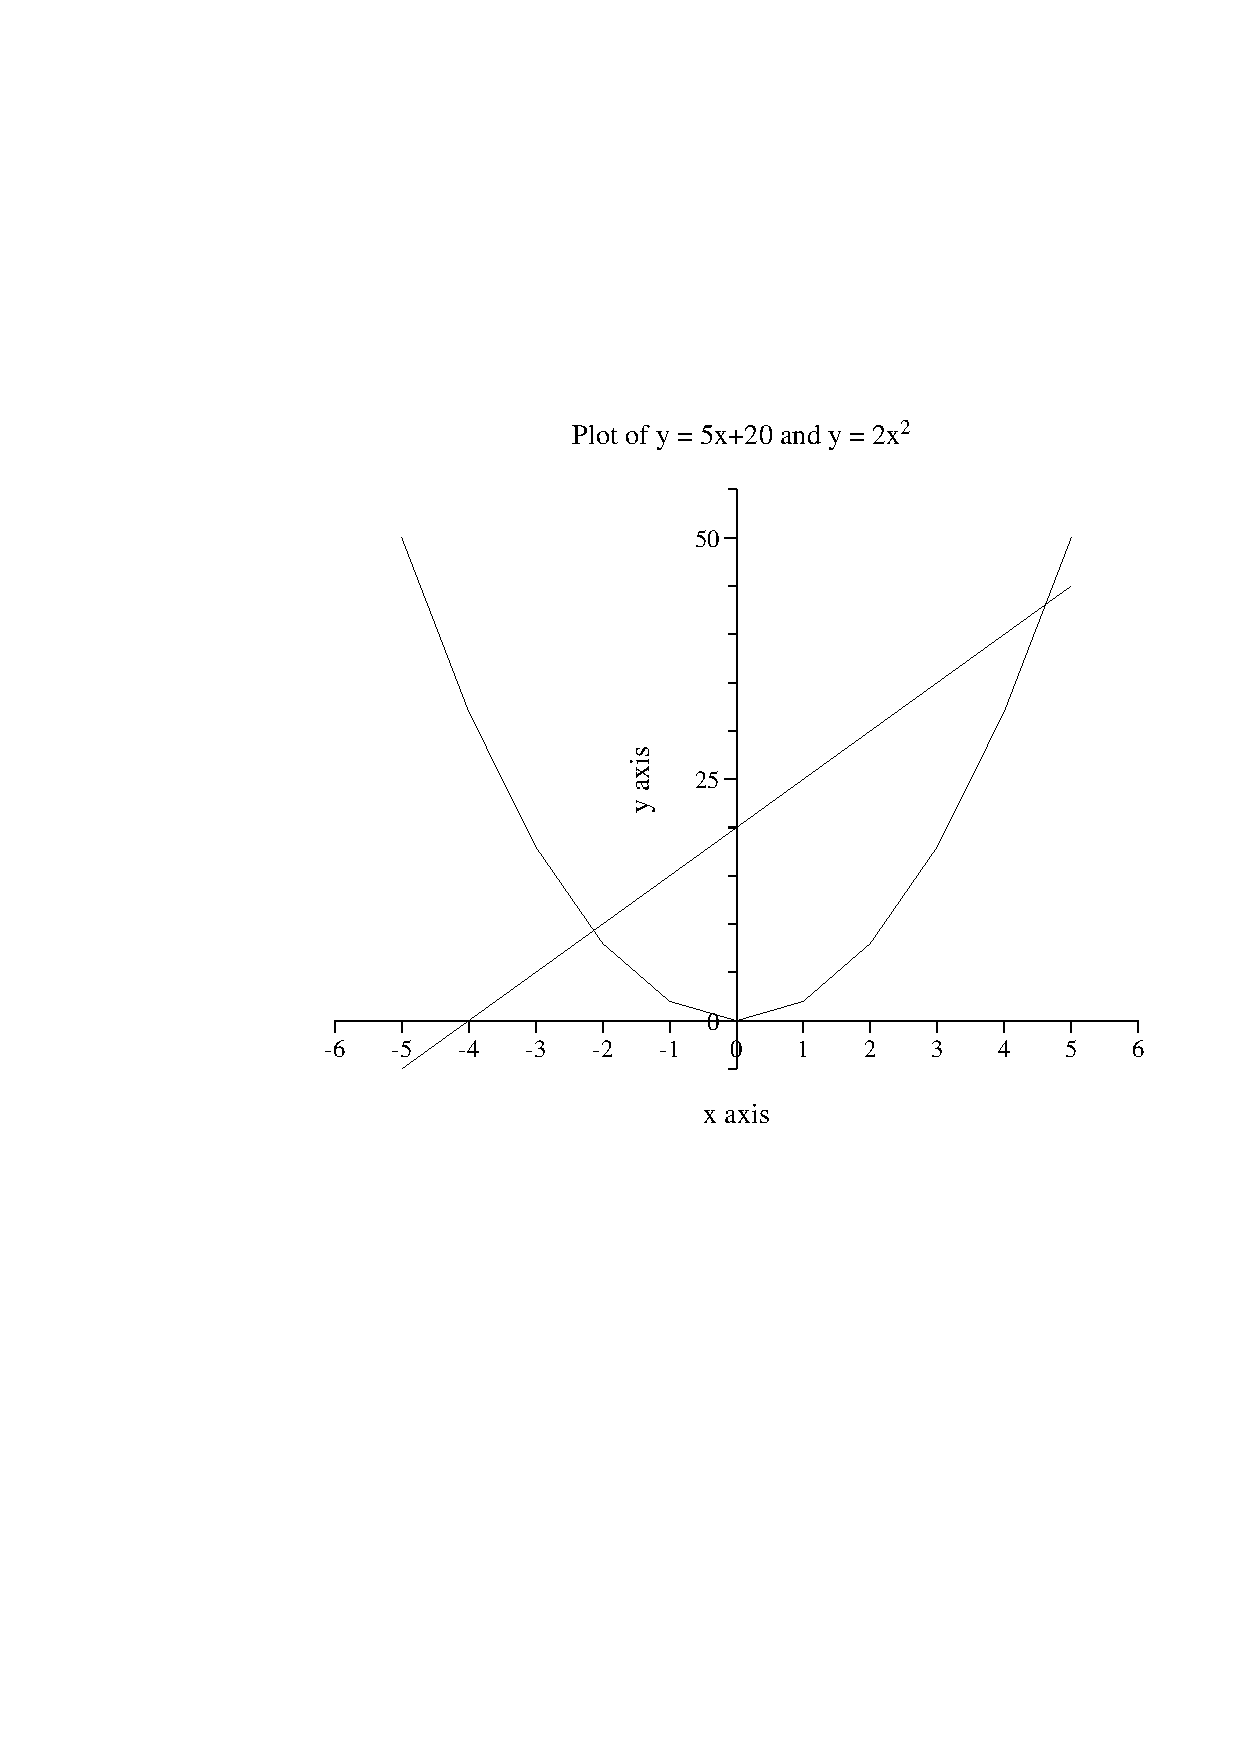
\epsfig{file=figure7,height=8cm}} &
{\vspace{-8cm}
{\em Data}
\vspace*{3mm}

\begin{boxedverbatim}
-5 50 -5
-4 32 0
-3 18 5
-2 8 10
-1 2 15
0 0 20
1 2 25
2 8 30
3 18 35
4 32 40
5 50 45
\end{boxedverbatim}
}
\end{tabular}
\end{center}
\caption[Overlaid plots]{Overlaid plots (see text for
explanation). \label{fig:example7}}
\end{figure}
In this example, the axis specifications for the plot
of $y = 2x^{2}$ are written into the format file {\tt example7.axes}:

\begin{center}
\begin{boxedverbatim}
plt example7.data 0 1 -f example7.format
\end{boxedverbatim}
\end{center}
where {\tt example7.format} contains:
\begin{center}
\begin{boxedverbatim}
t Plot of y = 5x+20 and y = 2x
L (P*.8) - - LB 2
x x axis
y y axis
xa -6 6 1 - 1 0
ya -5 55 5 - 5 0
fa example7.axes
\end{boxedverbatim}
\end{center}

\index{point size}%
\index{character size}%
\index{type size}%
\index{subscripts}%
\index{superscripts}%
{\small
[In {\tt example7.format}, the second line ({\tt L (P*.8) - - LB 2})
appends a small superscript 2 to the plot title.  {\tt (P*.8)} reduces the
point size to 80\% of the default, and ``{\tt- - LB"}'' aligns the
left bottom point of the 2 at the {\tt RC} point of the previous string
(the title).  See chapter~\ref{sec:font-groups} for a discussion of
how text styles, including point size, can be modified;  and see
chapter~\ref{sec:labelling} for details on the {\tt -L} option and on
creating superscripts and subscripts in plot titles and other text.]}

\index{f@{\tt -f} (format file) option}%
The information written by the command above into {\tt example7.axes}
is recalled in the command below (using the {\tt -f} option), and the
new plot is then overlaid using the {\tt -o} option.

\begin{center}
\begin{boxedverbatim}
plt example7.data 0 2 -f example7.axes -o
\end{boxedverbatim}
\end{center}

\index{fa@{\tt -fa} (save axis setup in file) option}%
\index{xa@{\tt -xa} (set up x axis) option}%
\index{ya@{\tt -ya} (set up y axis) option}%
\index{X@{\tt -X} (set x axis limits) option}%
\index{Y@{\tt -Y} (set y axis limits) option}%
Although a single data file, {\tt example7.data}, contains data for both plots
in this example, the data might just as easily have been collected from
different files.  Note that if you know ahead of time what axis limits you will
use, you don't need {\tt -fa}; just use {\tt -xa}, {\tt -ya}, {\tt -X}, or {\tt
-Y} with the appropriate axis limits when making the second plot.

\section{Legends \label{sec:legends}}

\index{legend}%
\index{line style}%
A legend (also known as a key) is useful when two or more data plots are drawn
on the same axes, as in the previous section.  A legend typically includes {\em
sample plot segments} (short segments drawn using the same line styles used for
the data plots), each of which is followed by {\em legend text} (typically a
description of the associated plot).  Figure~\ref{fig:example10} illustrates a
plot that includes a boxed legend.

\index{le@{\tt -le} (define legend entry) option}%
\index{lp@{\tt -lp} (set up legend box) option}%
The {\tt -lp} option is used to specify the location for the legend,
and the {\tt -le} option is used to define an entry to be shown as
part of the legend.  These options take their arguments as follows:

\begin{quote}
{\tt -lp} \emph{xw0 yw0 boxscale seglength opaque}\\
{\tt -le} \emph{linenumber plotnumber text}
\end{quote}

\index{window coordinates}%
The first two arguments of {\tt -lp} define the window coordinates of
the upper left corner ({\tt LT}) of the legend text.  {\tt plt} draws
a box around the legend text, determining the width and height of the
box based on the size of the text and sample plot segments it
encloses, but you can adjust the width of the box using the optional
{\em boxscale} argument (which is a factor that multiplies the width
calculated by {\tt plt}).  Thus a {\em boxscale} of 1.05 creates a box
5\% larger than the default size; as a special case, a {\em boxscale}
of 0 suppresses the box entirely.  The optional {\em seglength}
argument tells {\tt plt} how long to make the sample plot segments in
the legend, as a fraction of the x axis length (by default, {\tt plt}
draws these segments so that they are 5\% of the length of the x
axis).  If {\em opaque} is {\tt yes} (default), the background of the
legend box is opaque white;  otherwise, the legend box is transparent
(any previously drawn material remains visible through the legend box).

\index{line style}%
The first argument of {\tt -le} specifies the line number of the entry
within the legend (the top line is line number 0).  Each plot drawn by
{\tt plt} has an implicit {\em plotnumber} (the first has a {\em
plotnumber} of 0); this is the second argument of {\tt -le}, used to
determine the line style for the entry's sample plot segment).  The
third and final argument of {\tt -le} is the text to be shown next to
the sample plot segment.

\begin{figure}
\begin{center}
\fcolorbox{blue}{white}{
\epsfig{file=figure10,height=10cm}}
\end{center}
\caption[Making legends with symbols]{See section~\ref{sec:legends}, {\em
Legends}, for details on how this plot was created.
\label{fig:example10}}
\end{figure}

Study figure~\ref{fig:example10} to see how these options work.
This plot was produced using the command
\begin{center}
\begin{boxedverbatim}
plt example10.data % -f example10.format
\end{boxedverbatim}
\end{center}
where the data file, {\tt example10.data}, was produced by this program
fragment:
\begin{center}
\begin{boxedverbatim}
for (i = 0; i < 20; i++)
    printf("%d %.3lf %.3lf %.3lf\n",
           i,
           sin(0.4*i*PI) + 1.5,
           (double)random()/(double)RAND_MAX + 3.8,
           .1 + 0.15*(double)random()/(double)RAND_MAX);
\end{boxedverbatim}
\end{center}
and  {\tt example10.format} contains:
\begin{center}
\begin{boxedverbatim}
t Making Legends with Symbols
x X Axis Units
xa 0 20 1
ya 0 5

# Move the y axis slightly to the left.
yo .02

# Make four plots on the same set of axes.
p 0,1n(W5,L1) 0,1S1 0,2n(W12,G.8) 0,2,3E0

# Put legend text at window coordinates (.67,.64) and
# widen the legend box by 5%.
lp .67 .64 1.05

# Describe plot 2 in the top line (line 0) of the legend.
le 0 2 Random Series

# Plot 3 is the same as plot 2, but with a different
# plotstyle (using symbols).  By using a second "le"
# command for line 0 here, we create a sample plot
# segment that is composed by overlaying the two
# plotstyles.  The text has already been supplied in
# the previous command, so it is omitted here.
le 0 3

# The plot number is omitted from the next "le" command,
# because the text that is to appear on line 1 of the
# legend is a continuation of the description of the
# data in line 0.  The "-" means that no sample data
# segment will be drawn when this command is executed.
le 1 - (Synthesized)

# Describe plots 0 and 1.
le 2 0 Sine Function
le 2 1
\end{boxedverbatim}
\end{center}

(The {\tt -yo} option is described in chapter~\ref{sec:ax2}.)
The line beginning with ``{\tt p~0}...'' makes four plots using
several different plot styles:

\begin{itemize}
\item Plot number 0 ({\tt 0,1n(W5,L1)}) plots columns 0 and 1 in normal plot
({\tt n}) style, using a line width of 5 ({\tt W5}, slightly broader than the
default, 3 or 4) and a dotted line ({\tt L1}).  
\item Plot number 1 ({\tt 0,1S1}) replots columns 0 and 1, this time as
a scatter plot ({\tt S1}), where the ``{\tt 1}'' indicates the use of
symbol number 1 (an open inverted triangle).
\item Plot number 2 ({\tt 0,2n(W12,G.8)}) plots columns 0 and 2 in
normal plot style, using a broad line ({\tt W12}) drawn in 80\% grey
({\tt G.8}).
\item Plot number 3 ({\tt 0,2,3E0}) replots columns 0 and 2 as a
scatter plot with error bars from column 3, using symbol number 0
(an open circle).
\end{itemize}

{\em Transient fontgroup modifications} such as ``{\tt
(W5,L1)}'' and ``{\tt (W12,G.8)}'' are described in detail in
chapter~\ref{sec:font-groups}.  Note that the order of the overlay
affects the appearance; since the open symbols (numbers 0 through 4)
used in plots 1 and 3 have opaque centers, they appear differently if
drawn on top of (after) other elements than if drawn below (before)
those elements.

\section{Placing multiple plots on a page \label{sec:plot-windows}}

\index{W@{\tt -W} (define plot window on page) option}%
\index{w@{\tt -w} (use predefined plot window) option}%
\index{subplots}%
In this section, the concept of using multiple windows within a single
screen or page is introduced.  You will need to become familiar with
the following options:

\begin{quote}
{\tt -W} \emph{xp0 yp0 xp1 yp1}\\
{\tt -w} \emph{type subsection}
\end{quote}

\index{page coordinates}%
The arguments of the {\tt -W} option are the {\em page coordinates} of
the lower left $(xp0,yp0)$ and upper right $(xp1,yp1)$ corners of the
plot window.  (Recall that the default plot window, which fills the
entire page or screen, has corners with page coordinates $(0,0)$ and
$(1,1)$.)  All output is scaled to fit within this window.  

Study figure~\ref{fig:example16}, in which the {\tt -W} option is used to scale
entire plots and the {\tt -s e} option (see chapter~\ref{sec:suppress}) is
used to suppress erasure so that the plots appear on the same page.

\begin{figure}
\begin{center}
\fcolorbox{blue}{white}{
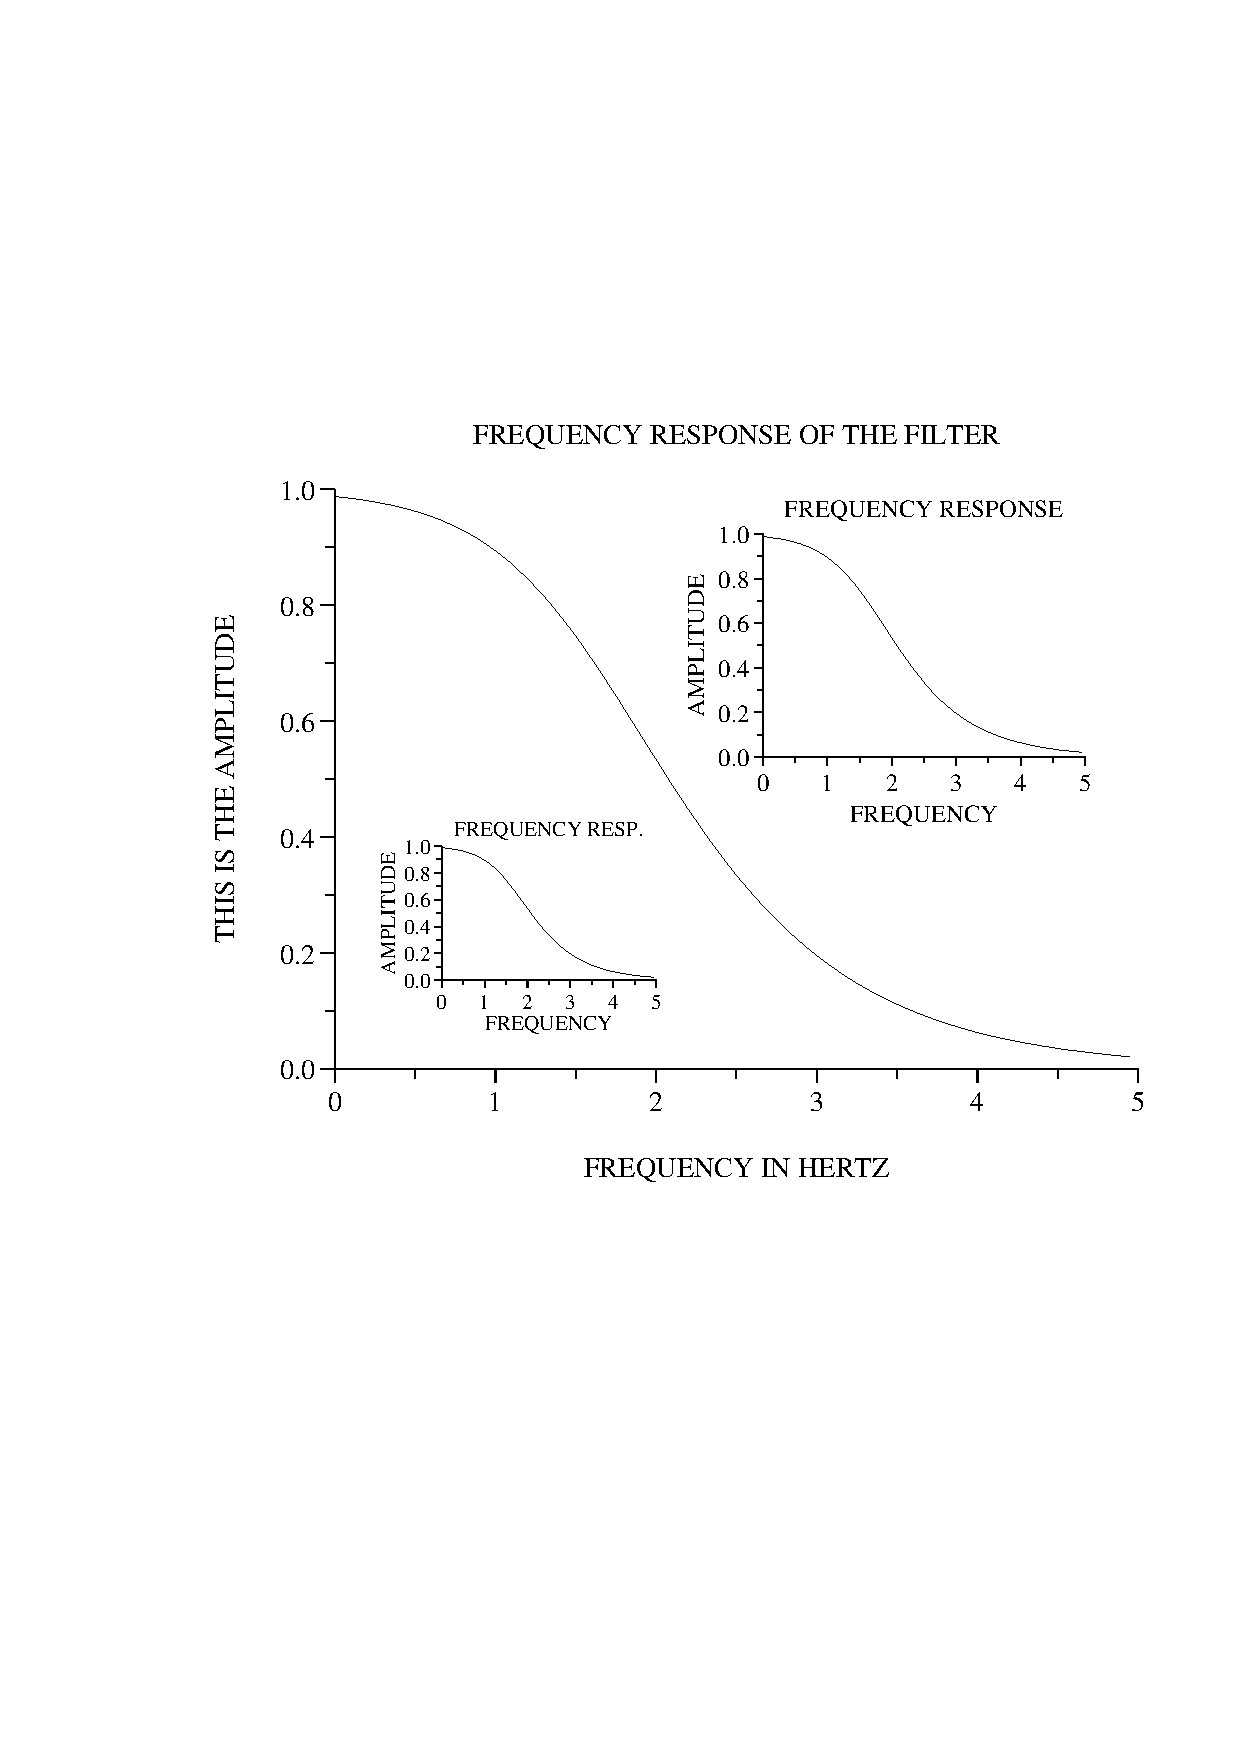
\epsfig{file=figure16,height=10cm}}
\end{center}
\caption[Scaling and placement]{This example demonstrates how a plot can be
scaled and placed on the page; it was produced using these commands:
\label{fig:example16}}
\begin{center}
\begin{boxedverbatim}
plt ldemo.data 2 3 -t"FREQUENCY RESPONSE OF THE FILTER" \
 -x"FREQUENCY IN HERTZ" -y"THIS IS THE AMPLITUDE" -sf all P16
plt ldemo.data 2 3 -t"FREQUENCY RESP." -x"FREQUENCY" \
 -y"AMPLITUDE"  -W .3 .3 .5 .45 -se -sf all P12
plt ldemo.data 2 3 -t"FREQUENCY RESPONSE" -x"FREQUENCY" \
 -y"AMPLITUDE"  -W .6 .55 .9 .8 -se -sf all P14
\end{boxedverbatim}
\end{center}
\end{figure}

The {\tt -w} option can address several windows that have been
predefined for convenience.  The first argument of {\tt -w} may be
{\tt m} (a single window that fits within a frame to be described
shortly), {\tt b} (one of two windows covering either the top or
bottom of the page), or {\tt q} (one of four windows covering the
upper left, upper right, lower left, or lower right quadrant of the
page).  The variant types {\tt ms}, {\tt bs}, and {\tt qs} are windows
of reduced size to allow extra room for axis labels.  Use the {\em
subsection} argument (which may have values 0, 1, 2, 3, or 4) to
specify which window is to be used for the current plot.  By
convention, subsection 0 is used to start a new page (erase the
screen) and to draw a grid and a title for the page.  When using
subsections 1, 2, 3, or 4, the plot is drawn on the current page
without erasing anything that may have been plotted there already.

Figures~\ref{fig:example11}, \ref{fig:example12}, and \ref{fig:example13}
illustrate the use of {\tt -wm}, {\tt -wb}, and {\tt -wq} respectively.  All
three use the data file {\tt example11.data}, which contains:
\begin{center}
\begin{boxedverbatim}
0 0 0 9 1
1 3 1 6 0
2 2 2 7 1
3 4 3 4 2
4 3 4 5 3
5 5 3 3 4
6 4 2 4 3
7 7 1 2 2
8 6 0 3 1
9 9 1 0 0
\end{boxedverbatim}
\end{center}

\begin{figure}[h]
\begin{center}
\fcolorbox{blue}{white}{
\epsfig{file=figure11,height=10cm}}
\caption[Single-window framed plot]{This plot was created using the commands:
\label{fig:example11}}

\begin{boxedverbatim}
plt -wm 0 -t "This is the main title for the plot"
plt example11.data 0 1 -wm 1 -t "Window 1"
\end{boxedverbatim}
\end{center}
\end{figure}

\begin{figure}
\begin{center}
\fcolorbox{blue}{white}{
\epsfig{file=figure12,height=10cm}}
\caption[Two-window framed plot]{This plot was created using the commands:
\label{fig:example12}}

\begin{boxedverbatim}
plt -wb 0 -t "This is the main title for the plot"
plt example11.data 0 1 -wb 1 -t "Window 1"
plt example11.data 0 2 -wb 2 -t "Window 2"
\end{boxedverbatim}
\end{center}
\end{figure}

\begin{figure}
\begin{center}
\fcolorbox{blue}{white}{
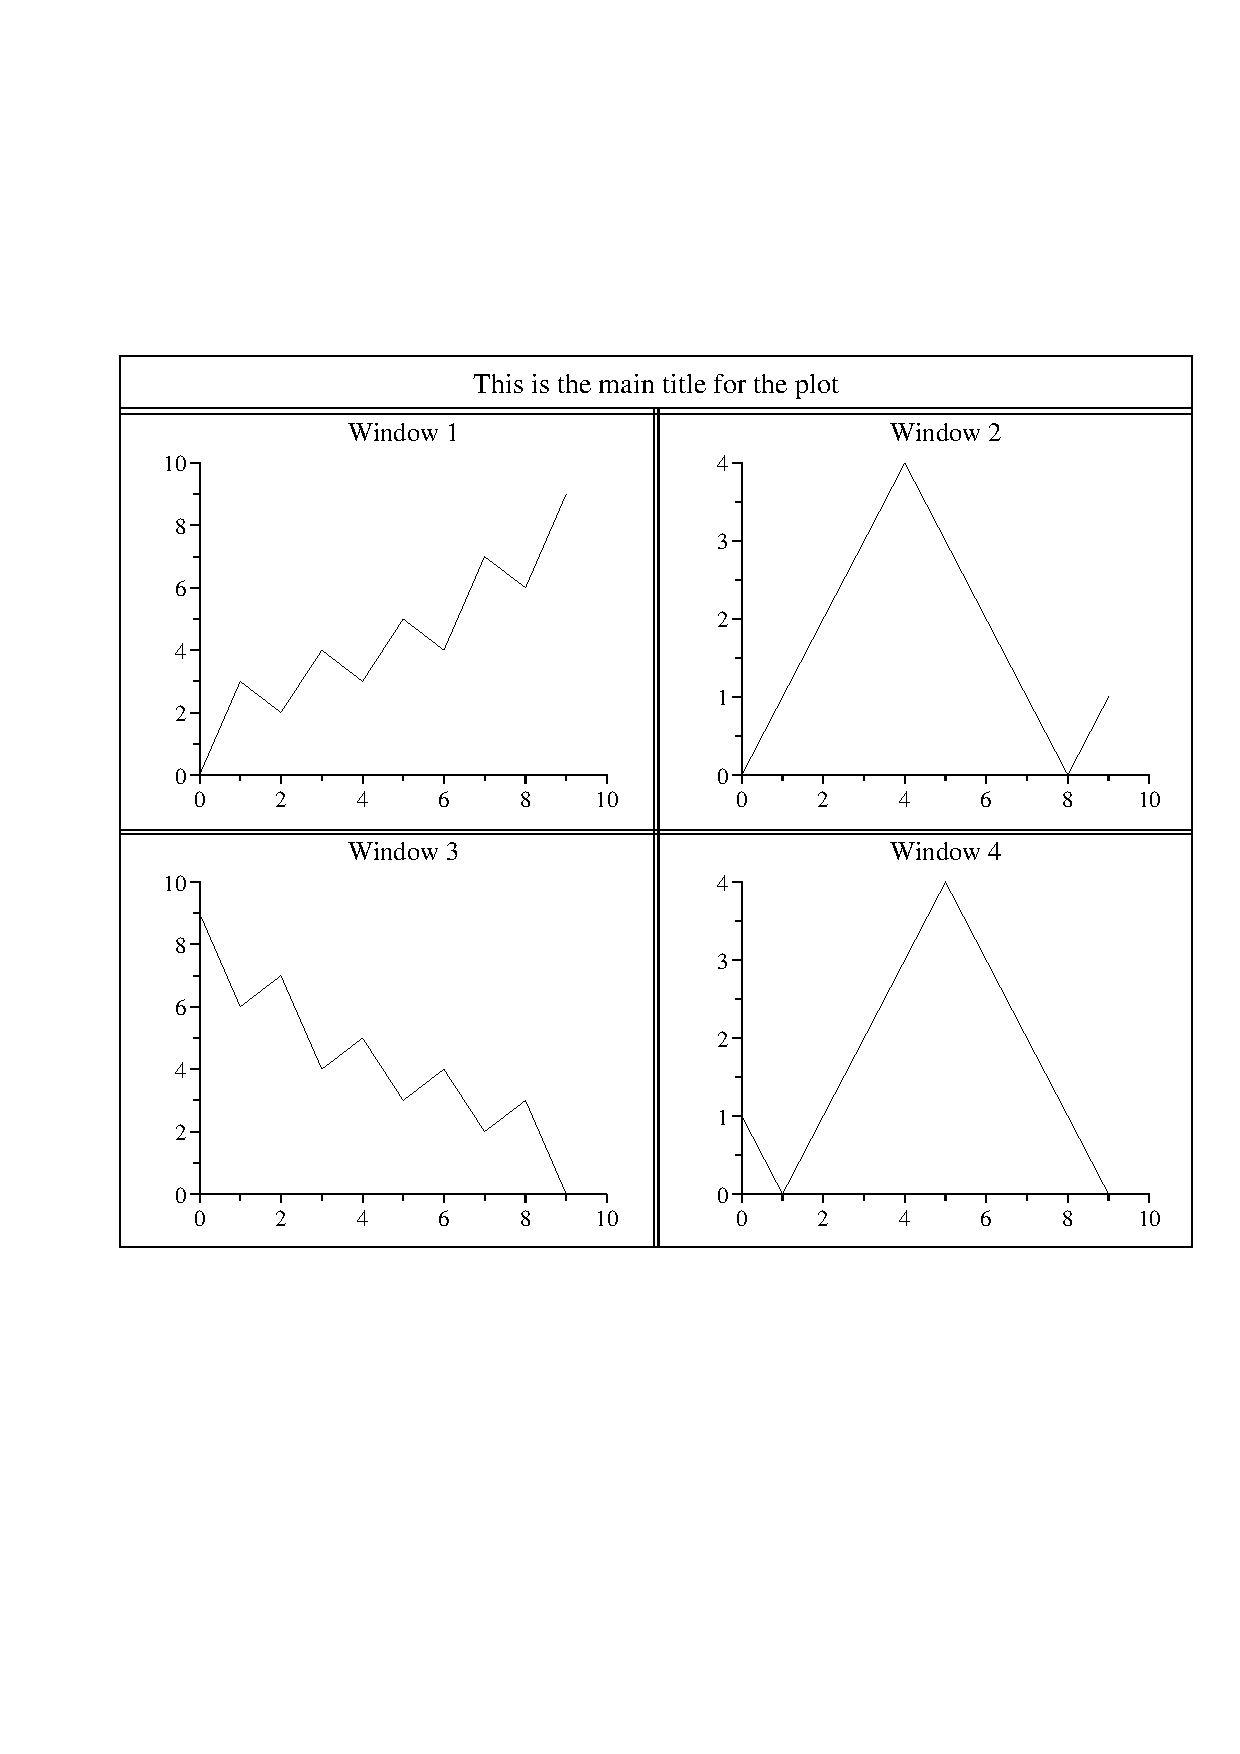
\epsfig{file=figure13,height=10cm}}
\caption[Four-window framed plot]{This plot was created using the commands:
\label{fig:example13}}

\begin{boxedverbatim}
plt -wq 0 -t "This is the main title for the plot"
plt example11.data 0 1 -wq 1 -t "Window 1"
plt example11.data 0 2 -wq 2 -t "Window 2"
plt example11.data 0 3 -wq 3 -t "Window 3"
plt example11.data 0 4 -wq 4 -t "Window 4"
\end{boxedverbatim}
\end{center}
\end{figure}

\index{character size}%
\index{ch@{\tt -ch} (character resize) option}%
When reducing the size of a plot, it is often desirable to avoid rescaling
any text in the plot, so that it remains readable.  The {\tt -ch} option
makes this possible:

\begin{description}
\item[{\tt -ch} {\em height-factor width-factor}]
Use this option to resize text;  the arguments specify factors by which the
normal height and width of characters output by {\tt plt} are to be enlarged
(or reduced, if a factor is less than 1).
\end{description}

\chapter{Labelling Your Plot \label{sec:labelling}}

\index{hl@{\tt -hl} (horizontal label from file) option}%
\index{vl@{\tt -vl} (vertical label) option}%
\index{text box coordinates}%
\index{window coordinates}%
The {\tt -hl} and {\tt -vl} options allow you to create horizontal and vertical
labels anywhere within your plot, using window coordinates, $(xw,yw)$, to
specify the location for the label; and a text box coordinate, {\em tbc} (e.g.,
``{\tt CB}'', ``{\tt RT}'', etc.), to specify which point in the text box
should coincide with $(xw,yw)$. These options take their arguments as follows:

\begin{quote}
{\tt -hl} \emph{xw yw tbc nlines file}\\
{\tt -vl} \emph{xw yw tbc nlines file}
\end{quote}

All arguments are optional (but if a specified argument follows an
omitted argument, you must supply a ``{\tt -}'' as a placeholder for
the omitted argument).  If $xw$ or $yw$ is omitted, the missing
coordinate is set to that of the {\tt RC} point of the previous
label, allowing labels to be concatenated (see below).  If
{\em tbc} is omitted, the default value is ``{\tt CC}'', i.e., the
label will be centered on $(xw,yw)$.  If specified, {\em nlines} is a
number indicating how many input lines are to be used to form the
label (line breaks are reproduced by {\tt plt} as they appear in the
input).

If {\em file} is specified, the text for the label is read from the first
{\em nlines} lines of {\em file}.  If {\em nlines} is not specified, the
entire contents of {\em file} are used for the label.

\index{f@{\tt -f} (format file) option}%
\index{F@{\tt -F} (format string) option}%
If {\em file} is not specified, the next {\em nlines} lines of the {\tt plt -f}
format file or {\tt plt -F} format string form the label; in this case, if {\em
nlines} is also not specified, the label is formed from only one line (the next
line) of the format file or string.

\index{L@{\tt -L} (horizontal label from string) option}%
\index{l@{\tt -l} (horizontal label from string) option}%
The {\tt -L} and {\tt -l} options can be used in a similar way to create
horizontal labels.  The arguments for these options are supplied as follows:

\begin{quote}
{\tt -L} \emph{xw yw tbc text}\\
{\tt -l} \emph{x y tbc text}
\end{quote}

\index{text box coordinates}%
\index{window coordinates}%
\index{data coordinates}%
As for {\tt -hl}, the {\em tbc} argument is one of the twelve named text box
coordinates.  The {\em text} argument is the string to be used for the label;
it may include whitespace, but it ends at the end of the line on which it
appears.  The difference between {\tt -L} and {\tt -l} is that the former
takes window coordinates $(xw,yw)$, and the latter takes data coordinates
$(x,y)$.

These options are demonstrated in figure~\ref{fig:example9}, which uses the
format file {\tt example9.format}, containing:
\begin{center}
\begin{boxedverbatim}
xa 0 600
ya 0 500
x Time Between Stimulations (msecs)
y Refractory Period (msecs)
# Note: the next line ends with a lower-case L, not a numeral 1!
p 0,1,2,3l
t ch 1.2
l 400 200 CC fires every beat
L .1 .9 CC . . .
hl .45 .81 CC 2
fires every
other beat
hl .25 .92 - 4
  fires
 every
third
beat
\end{boxedverbatim}
\end{center}
and the data file {\tt example9.data}, containing:
\begin{center}
\begin{boxedverbatim}
0 0 500 500
0 0 250 500
0 0 166 500
0 0 125 500
0 0 100 500
\end{boxedverbatim}
\end{center}

\begin{figure}
\begin{center}
\fcolorbox{blue}{white}{
\epsfig{file=figure9,height=10cm}}
\end{center}
\caption[Labelling a plot]{Labelling a plot \label{fig:example9} using the {\tt
-hl}, {\tt -l}, and {\tt -L} options.  This plot was produced using the
command}
\begin{center}
\begin{boxedverbatim}
plt example9.data % -f example9.format
\end{boxedverbatim}
\end{center}
\end{figure}

\index{data coordinates}%
\index{window coordinates}%
In figure~\ref{fig:example9}, notice especially how whitespace at the beginning
of two lines in the second {\tt hl} option's text is preserved in the plot.
Note also how both data and window coordinates are used with several {\tt plt}
options.  The next chapter describes several more options that can be used in
the same way.  Options {\tt -A}, {\tt -B}, {\tt -C}, {\tt -D}, {\tt -L}, {\tt
-hl}, {\tt -vl}, {\tt -le}, and {\tt -lp} accept window coordinates; options
{\tt -a}, {\tt -b}, {\tt -c}, {\tt -d}, and {\tt -l} accept data coordinates.
For now, note that you often have a choice of using data or window coordinates,
since many of these options come in two varieties: upper-case options that use
window coordinates, and similar lower-case options that use data coordinates.

\section{Concatenating labels \label{sec:concatenation}}

\index{font}%
\index{subscripts}%
\index{superscripts}%
Labels can be concatenated if you wish to incorporate font changes,
subscripts or superscripts, or other special effects in labels.  The
plot title in figure~\ref{fig:example7}, page~\pageref{fig:example7},
illustrates how this can be done.  {\tt plt} keeps track of the {\tt
RC} point of each label, and uses these coordinates in place of
omitted $(x,y)$ or $(xw,yw)$ coordinates in label options.  If the
coordinates are omitted from the first label in any given plot, the
{\tt RC} point of the plot title is used to determine the label
coordinates.

\index{color}%
This facility would be of little use if it were not possible to change
the style used by {\tt plt} for rendering the text of labels.  This
can be done using {\em fontgroup substitution}, as described in detail
in chapter~\ref{sec:font-groups}, beginning on
page~\ref{sec:font-groups}.  In a nutshell, what you do is to describe
the style you want in an extra argument that is enclosed in
parentheses and that immediately follows the option name, as in:
\begin{center}
\begin{boxedverbatim}
-L (Ft-b-i,P20,Cmaroon) .5 .5 CC Marooned!
\end{boxedverbatim}
\end{center}
(This sets the label ``Marooned!'' in 20-point Times Bold Italic of an
appropriate color.)

\index{font}%
\index{text box coordinates}%
If you wish simply to concatenate labels, perhaps changing the font or
text color, use {\tt LC} as the text box coordinate for the second
(and subsequent) labels, as in:
\begin{center}
\begin{boxedverbatim}
-L (Cblue,Fh) .4 .7 CC Hello,
-L (Cgreen,Fh-o) - - LC " World!"
\end{boxedverbatim}
\end{center}
These commands produce a blue Helvetica ``Hello,'' centered on window
coordinates (.4,.7) followed by a green Helvetica-Oblique ``World!''.
Note that the entire string is not centered on (.4,.7);  if you want
to center a multi-part label you will need to do some experimentation.
Also note the use of quotation marks to force the inclusion of the
initial space before ``World!''.

In the following example, Greek and Roman letters are mixed to produce
the equation $\mathrm{y = A\, sin ( \omega t + \phi )}$:
\begin{center}
\begin{boxedverbatim}
-L .3 .5 CC y = A sin(
-L (Fs) - - LC w
-L - - LC "t + "
-L (Fs) - - LC f
-L - - LC )
\end{boxedverbatim}
\end{center}

\index{point size}%
\index{character size}%
\index{type size}%
\index{text box coordinates}%
\index{subscripts}%
\index{superscripts}%
To create a subscript or subscript, use {\tt LN} or {\tt LB}
respectively as the text box coordinate for the label containing the
subscript or superscript, and use {\tt LB} or {\tt LN} to return to
the original baseline afterwards.  It is often effective to reduce the
point size of superscripts and subscripts, as in this example, which produces
$y = x^{\alpha} + x_{0}{\beta}$:
\begin{center}
\begin{boxedverbatim}
L .6 .3 LC y = x
L (Fs,P*.8) - - LB a
L - - LN " + x"
L (P*.8) - - LN 0
L (Fs) - - LB b
\end{boxedverbatim}
\end{center}
The same effects are possible in a vertical label, as in this example:
\begin{center}
\begin{boxedverbatim}
vl .6 .5 LC 1 -
y = x
vl (Fs,P*.8) - - LB 1 -
a
vl - - LN 1 -
 + x
vl (P*.8) - - LN 1 -
0
vl (Fs) - - LB 1 -
b
\end{boxedverbatim}
\end{center}

\begin{figure}
\begin{center}
\fcolorbox{blue}{white}{
\epsfig{file=labels,height=8cm}}
\end{center}
\index{superscripts}%
\caption{Labels with superscripts and font changes \label{fig:labels}}
\end{figure}

See figure~\ref{fig:labels} for examples of this technique.  This
figure was created using the command
\begin{center}
\begin{boxedverbatim}
plt cos2.data 0 1 -f labels.format
\end{boxedverbatim}
\end{center}
where {\tt cos2.data} was created using this program fragment:
\begin{center}
\begin{boxedverbatim}
for (i = -180; i <= 180; i += 5) {
    c = cos(M_PI*i/180.0);
    printf("%d %g\n", i, c*c);
}
\end{boxedverbatim}
\end{center}
and {\tt labels.format} contains:
\begin{center}
\begin{boxedverbatim}
xa -180 180 15 - 3
ya 0 1

# Set the first part of the plot title using the -t option.
t Plot of y = cos
# Concatenate the remaining pieces using -L options.
L (P*.8) - - LB 2
L - - LN (
L (Fs) - - LC q
# "q" in Symbol font is theta.
L - - LC )

# Avoid drawing a normal x-axis label.
x ""
# Instead of a normal x-axis label, draw this label using
# the -L option with ym = -.16, to put it in the same
# position as a normal x-axis label.
L (Fs) .425 -.16 LC q
L - - LC " (degrees)"

# Similarly, draw this label using -vl with xm = -.115 to put it
# in the same position as a normal y-axis label.  (We don't need
# to suppress the normal y-axis label, because plt produces one
# only if requested explicitly.)
vl -.115 .44 LC 1 -
cos
vl (P*.8) - - LB 1 -
2
vl - - LN 1 -
(
vl (Fs) - - LC 1 -
q
vl - - LC 1 -
)
\end{boxedverbatim}
\end{center}

\index{subscripts}%
\index{superscripts}%
Another way to create subscripts and superscripts is to specify an
appropriate $y$ or $yw$ while omitting the x coordinate (for
horizontal labels).  Some experimentation may be needed to achieve the
desired results.

These methods cannot be used directly to concatenate text in axis labels.
If you need to do this, suppress {\tt plt}'s standard axis label,
either by supplying an empty string as the argument for {\tt -x} or {\tt -y},
or by using the appropriate {\tt -s} option (see chapter~\ref{sec:suppress});
then create your own axis label using the options described above.

\chapter{Drawing Line Segments, Arrows, and Boxes \label{sec:lines-arrows}}

Well-chosen annotations can make a good plot better.  In the previous
chapter, we saw how labels can be placed anywhere on a plot, using
either data or window coordinates.  {\tt plt} also allows you to draw
arbitrary line segments, arrows, and boxes on your plot.

\index{c@{\tt -c} (connect data coordinates) option}%
\index{C@{\tt -C} (connect window coordinates) option}%
\index{data coordinates}%
\index{window coordinates}%
Use the {\tt -C} and {\tt -c} (connect) options to draw arbitrary line
segments, as follows:

\begin{quote}
{\tt -C} \emph{xw0 yw0 xw1 yw1}\\
{\tt -c} \emph{x0 y0 x1 y1}
\end{quote}

These options connect the two points specified by their arguments with a
line segment.  The {\tt -C} option connects the points with window
coordinates $(xw0,yw0)$ and $(xw1,yw1)$.  The {\tt -c} option connects
the points with data coordinates $(x0,y0)$ and $(x1,y1)$.

\index{a@{\tt -a} (arrow in data coordinates) option}%
\index{A@{\tt -A} (arrow in window coordinates) option}%
The {\tt -A} and {\tt -a} (arrow) options work in the same way as {\tt
-C} and {\tt -c}, respectively, but they also draw an arrowhead
pointing toward the first specified point, $(xw0,yw0)$ or $(x0,y0)$:

\begin{quote}
{\tt -A} \emph{xw0 yw0 xw1 yw1}\\
{\tt -a} \emph{x0 y0 x1 y1}
\end{quote}

\index{point size}
Note that the size of the arrowhead is determined by the specified
point size in the figure ({\tt f}) font group, or in local override
instructions (see figure~\ref{fig:example14}).

\index{b@{\tt -b} (box in data coordinates) option}%
\index{B@{\tt -B} (box in window coordinates) option}%
The {\tt -B} and {\tt -b} (box) options similarly accept arguments
specifying two points, but in this case the points are diagonally
opposite corners of a box (rectangle) that is to be drawn:

\begin{quote}
{\tt -B} \emph{xw0 yw0 xw1 yw1}\\
{\tt -b} \emph{x0 y0 x1 y1}
\end{quote}

\index{d@{\tt -d} (filled box in data coordinates) option}%
\index{D@{\tt -D} (filled box in window coordinates) option}%
\index{color}%
\index{grey level}%
The {\tt -D} and {\tt -d} (dark box) options work in the same way as
{\tt -B} and {\tt -b} respectively, but boxes drawn when using these
options are filled.  The filling is black by default, but may be changed
by setting the grey level or color in the {\tt f} (figure) font group
(see figure~\ref{fig:colors}).

\begin{quote}
{\tt -D} \emph{xw0 yw0 xw1 yw1}\\
{\tt -d} \emph{x0 y0 x1 y1}
\end{quote}

Remember that in each case, as with {\tt -L} and {\tt -l}, the upper
case version of the option takes window coordinates, and the lower
case version takes data coordinates.

\begin{figure}
\begin{center}
\fcolorbox{blue}{white}{
\epsfig{file=flowchart,height=10cm}}
\end{center}
\caption{Line segments, arrows, and boxes \label{fig:flowchart}}
\end{figure}

These options are illustrated in figure~\ref{fig:flowchart}, which was
produced using the command:
\begin{center}
\begin{boxedverbatim}
plt -f flowchart.format
\end{boxedverbatim}
\end{center}
where the format file, {\tt flowchart.format}, contains:
\begin{center}
\begin{boxedverbatim}
# Define axis ranges, but don't draw the axes.
X 0 1
Y 0 1
s xy
# Use black, wide lines for figures by default.
sf f Cblack,W15,P20
# Draw labels in black 20 point Helvetica Bold.
sf l Cblack,P20,Fh-b
# Draw the plot title in 24 point Helvetica Bold.
t (Fh-b,P24) How to Hack
# Draw a green-outlined box and label it.
B (Cgreen) .1 .3 .3 .4
L .2 .35 CC Write
# Draw an arrow from the right edge of the box.
A .4 .35 .3 .35
# Draw a diamond using line segments, and label it.
C (Cred) .4 .35 .5 .45
C (Cred) .5 .45 .6 .35
C (Cred) .6 .35 .5 .25
C (Cred) .5 .25 .4 .35
L .5 .35 CC Done?
# Draw a line and arrow from the top of the diamond.
C .5 .45 .5 .7
A .4 .7 .5 .7
# Label the line and arrow.
L .51 .45 LB No
# Draw a filled light blue box.
D (CLightBlue) .2 .65 .4 .75
# Outline it in dark blue, and label it.
B (CDarkBlue) .2 .65 .4 .75
L .3 .7 CC Think!
# Draw a line and arrow from this box to the first.
C .2 .7 .15 .7
A .15 .4 .15 .7
# Draw an arrow from the right corner of the diamond.
A .7 .35 .6 .35
# Label the arrow.
L .6 .35 LT Yes
# Draw a filled box in 30% grey, and label it in white.
D (Cgrey30) .7 .3 .9 .4
L (Cwhite) .8 .35 CC Sleep
\end{boxedverbatim}
\end{center}

The {\tt -s} option, used in this example to suppress the axes, is
described in the next chapter.  The {\tt -sf} option, used to set the
default characteristics for the figures and labels in the example, is
discussed in chapter~\ref{sec:font-groups}, beginning on
page~\pageref{sec:font-groups}.

\chapter{Suppressing Plot Elements \label{sec:suppress}}

\index{s@{\tt -s} (suppress) option}%
The {\tt -s} option allows you to suppress (i.e., to avoid drawing)
selected features of your plots.  The sub-options following {\tt -s}
specify which elements to suppress.  The sub-options are as follows:

\begin{center}
\begin{tabular}{lp{10cm}}
{\tt e} & don't begin a new page (erase screen) before plotting \\
{\tt a} & suppress anything associated with axes \\
{\tt x} & suppress anything associated with the x axis \\
{\tt y} & suppress anything associated with the y axis \\
{\tt g} & suppress the grid \\
{\tt m} & suppress x axis and y axis tick marks \\
{\tt n} & suppress x axis and y axis tick mark numbers \\
{\tt t} & suppress titles for x axis, y axis, and graph \\
{\tt l} & suppress user-supplied labels ({\tt -hl}, {\tt -vl}, {\tt -l},
	 and {\tt -L} options) \\
{\tt p} & suppress all data plotting \\
{\tt f} & suppress all ``figures'' (boxes, line segments, arrows, and
	legends) \\
{\tt C} & enable all plot features (undo effects of previous {\tt -s}
	 sub-options) \\
{\tt X} & subsequent {\tt -s} sub-options apply only to the x axis \\
{\tt Y} & subsequent {\tt -s} sub-options apply only to the y axis \\
{\tt A} & subsequent {\tt -s} sub-options apply to both axes (default)
\end{tabular}
\end{center}

Two or more sub-options can be grouped, as in:

\begin{center}
\begin{boxedverbatim}
-s eg
\end{boxedverbatim}
\end{center}

By default, data points that fall outside of the axis limits are
suppressed.  If any data points are not plotted for this reason, {\tt
plt} produces a warning message indicating the number of points that
were excluded from the plot.  The {\tt -ex} option overrides this behavior:

\begin{description}
\index{ex@{\tt -ex} (don't exclude points) option}%
\item[{\tt -ex}]
Use this option to ensure that all data points that fall on the page will be
plotted.
\end{description}

\chapter{Colors, Line Styles, and Fonts \label{sec:font-groups}}

\index{color}%
\index{line style}%
The user can separately control how text and line segments are
rendered in five different contexts: axes and their numbering ({\tt
a}), figures (lines, boxes, and arrows, {\tt f}), labels ({\tt l}),
data plots ({\tt p}), axis and graph titles ({\tt t}), and all of
these at once ({\tt all}).  The contexts ({\tt a}, {\tt f}, {\tt l},
{\tt p}, and {\tt t}) are the five {\em predefined font groups}.  The
table below matches each of the predefined font groups with the {\tt
plt} options having related outputs.

\begin{center}
\begin{tabular}{ll}
\emph{Font group} & \emph{Options} \\ \hline
{\tt a} & {\tt xa}, {\tt ya}, {\tt X}, {\tt Y} (axes and numbering) \\
{\tt f} & {\tt A}, {\tt a}, {\tt B}, {\tt b}, {\tt C}, {\tt c}, {\tt
D}, {\tt d}, {\tt le}, {\tt lp} (figures and legends) \\
{\tt l} & {\tt L}, {\tt l}, {\tt hl}, {\tt vl} (labels) \\
{\tt p} & {\tt p} and sub-options (data plots) \\
{\tt t} & {\tt x}, {\tt y}, {\tt t} (titles)
\end{tabular}
\end{center}

A font group is defined by the following six parameters:

\begin{description}
\item[{\tt F}]
\index{font}%
font name (see figure~\ref{fig:fonts}), one of:
\begin{center}
\begin{tabular}{lp{2cm}|lp{2cm}|lp{2cm}}
{\tt c} & courier & {\tt h} & helvetica & {\tt t} & times \\
\hline
{\tt c-b} & courier-bold & {\tt h-b} & helvetica-bold & {\tt t-b} &
 times-bold \\
\hline
{\tt c-o} & courier-oblique & {\tt h-o} & helvetica-oblique & {\tt t-i} &
 times-italic \\
\hline
{\tt c-b-o} & courier-bold-oblique & {\tt h-b-o} & helvetica-bold-oblique &
 {\tt t-b-i} & times-bold-italic \\
\hline
{\tt s} & symbol
\end{tabular}
\end{center}

\item[{\tt P}]
\index{point size}%
\index{character size}%
\index{type size}%
point size (an integer $\ge 0$; 12 or 14 are normal point sizes)

\item[{\tt C}]
\index{color}%
color (see appendix~\ref{sec:color-names}, {\em Color Names}, beginning
on page~\pageref{sec:color-names})

\item[{\tt G}]
\index{grey level}%
grey level (see figure~\ref{fig:linestyles}); the grey level can be between
0.0 (black) and 1.0 (white)

\item[{\tt W}]
\index{line width}%
\index{width of line}%
line width (an integer $\ge 0$);  a normal line width is 3 or 4.  By
convention, a line width of 0 produces the narrowest possible line;  on
some high-resolution devices, such lines may not be visible, however.  See
figure~\ref{fig:linestyles}.

\item[{\tt L}]
\index{line style}%
line style (see figure~\ref{fig:linestyles}); select from the following
using either the number (0-4) or the one-word name:

\begin{center}
\begin{tabular}{ll}
0 & {\tt solid} \\
1 & {\tt dotted} \\
2 & {\tt shortdashed} \\
3 & {\tt dotdashed} \\
4 & {\tt longdashed}
\end{tabular}
\end{center}
\end{description}

\begin{figure}
\begin{center}
\fcolorbox{blue}{white}{
\epsfig{file=fonts,height=10cm}}
\end{center}
\caption{Samples of available fonts \label{fig:fonts}}
\end{figure}

\begin{figure}
\begin{center}
\fcolorbox{blue}{white}{
\epsfig{file=linestyles,height=10cm}}
\end{center}
\caption[Line styles and grey levels]{Line widths and styles, and grey
levels.  On very high resolution output devices, lines rendered with
zero width {\tt (W0)} may not be visible; a safer choice for a thin
line is {\tt (W1)}.  On older PostScript printers, however, zero-width lines
are usually visible because resolution is not too high, and they often
are rendered much faster than lines of any other width.  Note that
grey levels can also be specified using colors; for example, the
font group specification {\tt (Cgrey45)} is equivalent to {\tt (G.45)}.
\label{fig:linestyles}}
\end{figure}

\index{sf@{\tt -sf} (define font group) option}%
Use the {\tt -sf} option to define a font group or to modify the
parameters of a predefined font group:

\begin{quote}
{\tt -sf} {\em fontgroup specs ...}
\end{quote}

The {\em fontgroup} argument is the name of the font group; this can
be one of {\tt a}, {\tt f}, {\tt l}, {\tt p}, or {\tt t}, or you can
specify any other name you choose for a custom font group.  The {\em
specs} arguments can include any of the parameter names {\tt F}, {\tt
P}, {\tt C}, {\tt G}, {\tt W}, or {\tt L}, followed immediately by the
value to be given to the parameter;  separate parameters with commas.
For example, the following specifies that titles should be shown using
18-point Times Bold Oblique:

\begin{quote}
{\tt -sf t Ft-b-o,P18}
\end{quote}

\index{f@{\tt -f} (format file) option}%
Before it produces any output, {\tt plt} scans the entire command line
(and the format file, if {\tt -f} is used) for font group definitions
made using {\tt -sf}.  Thus the position of {\tt -sf} among the other
options makes no difference to the final result.

\index{p@{\tt -p} (plotstyle) option}%
{\em Fontgroup substitution} can be used to make {\tt plt} use any
desired fontgroup to control the appearance of any desired element.
Although each {\tt plt} option that renders text or graphics has an
associated font group that normally determines its appearance, any
other font group can take on this function if you substitute it
by naming it when using the option.  For most {\tt plt} options, do
this by supplying the font group's name in parentheses immediately
after the option, as in these examples:
\begin{center}
\begin{boxedverbatim}
-B "(p)" .1 .1 .3 .5
-L "(t)" .6 .4 CB "Group A (n=25)"
\end{boxedverbatim}
\end{center}
(The quotation marks should be omitted within a format file;  they are
needed on the command line to protect the parentheses from the shell.)
When using fontgroup substitution after a {\tt -p} option,
however, the font group name should follow the plotstyle specification,
as in:
\begin{center}
\begin{boxedverbatim}
-p "0,1Striangle(t)"
\end{boxedverbatim}
\end{center}

Even more flexibility is possible using {\em transient fontgroup
modifications}.  These can be performed using the same syntax as for
fontgroup substitutions, except that what goes inside the parentheses
is a list of fontgroup parameters, for example:
\begin{center}
\begin{boxedverbatim}
-D "(Cmagenta)" .1 .6 .2 .7
-p "0,1n(W3,Ldashed)"
\end{boxedverbatim}
\end{center}
Transient fontgroup modifications apply only to the option in which they
are defined.

In addition to absolute parameter values, as above, {\em relative
parameter values} may be supplied in a font group specification.
Relative parameter values are given in the form {\em $<$op$>N$}, where
{\em op} is one of the arithmetic operators ({\tt +}, {\tt -}, {\tt *}, or
{\tt /}) and $N$ is the amount by which the previous value of the parameter
is to be increased, decreased, multiplied, or divided respectively.  For
example, {\tt W*2} doubles the previous line width.

\begin{figure}[h!]
\begin{center}
\begin{tabular}{p{10cm}p{1.5cm}}
\fcolorbox{blue}{white}{
\epsfig{file=fontgroup1,height=8cm}} &
{\vspace{-85mm}\small{
{\em Data}
\vspace*{3mm}

\begin{boxedverbatim}
0 0.034
5 0.771
10 1.003
15 0.464
20 -0.393
25 -1.005
30 -0.798
35 0.027
40 0.760
45 0.980
50 0.432
55 -0.421
60 -0.988
65 -0.780
70 0.045
75 0.823
80 0.988
85 0.456
90 -0.470
95 -0.964
100 -0.830
\end{boxedverbatim}
}}
\end{tabular}
\end{center}
\caption[Using font group specifications]{This example illustrates the effects
of fontgroup redefinitions and substitutions, transient fontgroup
modifications, and the use of relative parameter values in fontgroup
specifications.  See the main text for details. \label{fig:fontgroup1}}
\end{figure}

\newpage

Figure~\ref{fig:fontgroup1} was created using:
\begin{center}
\begin{boxedverbatim}
plt example14.data -f fontgroup.format
\end{boxedverbatim}
\end{center}

The data file, {\tt example14.data}, contains 21 samples of a noisy sinusoid.
The format file, {\tt fontgroup.format}, contains:
\begin{center}
\begin{boxedverbatim}
# The entire format file is scanned for "sf" options before
# anything is rendered, so the x axis title is rendered in
# the font specified by the "sf t" option below.
x Time (seconds)

# Specify black 24-point Helvetica Bold for the "t" fontgroup.
# Although black is the default color, it needs to be specified
# explicitly (see below).
sf t Fh-b,P24,Cblack

# Specify red for the "p" fontgroup.
sf p Cred

# Here, a transient fontgroup modification (P/2) overrides the
# previously defined point size setting for the "t" font, so
# that the y axis title is rendered half as large as the
# (unscaled) x axis title.
y (P/2) Amplitude

# As shown in the previous line, if the argument following
# an option begins with "(", it is interpreted as a local
# fontgroup spec.  In order to use a string beginning with
# "(" as a string argument, it is necessary to quote it:
t "(Noisy) Sinusoid"
# Note that this title is rendered in 24-point type;  the
# effect of the local spec used earlier is limited to the
# line on which it appeared.

# Here, we make two plots, first a normal plot using the
# "p" fontgroup (in red), then a scatter plot using triangles.
# The effect of the "(t)" is to specify that the "t" fontgroup
# must be used for the second plot;  thus the triangles are
# black, not red, and are sized to match the 24-point type of
# fontgroup "t".
p 0,1n(p) 0,1Striangle(t)
# If, however, the color had not been specified explicitly
# for fontgroup "t", plt would not change the color between
# plots, and the triangles would be rendered in red.
\end{boxedverbatim}
\end{center}

\begin{figure}
\begin{center}
\fcolorbox{blue}{white}{
\epsfig{file=figure14,height=10cm}}
\end{center}
\caption[Creating special effects using font groups]{Font groups have been
redefined to create many of the special effects in this example. See the main
text for details. \label{fig:example14}}
\end{figure}

\newpage
Figure~\ref{fig:example14} shows several more complex uses of
different font groups.  This figure was produced using the command:
\begin{center}
\begin{boxedverbatim}
plt example14.data % -f example14.format
\end{boxedverbatim}
\end{center}
using the same data file as in the previous example.  The format file,
{\tt example14.\-format}, contains:
\begin{center}
\begin{boxedverbatim}
# Set font and point size for font group "l" (labels).
sf l Fs,P20

# Define two custom font groups, "fontgroup1" and "fontgroup2".
sf fontgroup1 W40,G.2
sf fontgroup2 Fh-b,P30,G.8

# Plot the data three times, first with a broad dark line,
# then with a medium light line, finally with open diamonds
# (symbol 2).
p 0,1n(fontgroup1) 0,1n(W10,G.8) 0,1S2

# Print the plot title.
t (fontgroup2) This is an example

# Local specifications are given below for the x and y axis
# titles.  These would override defaults for the predefined
# title (-sf t ...) font group had any been set.
x (Fc-o,P15) This is the x axis
y (Fc,P6) This is the y axis

# The label uses font group l defaults set above unless local
# instructions are given.  The choice of font "s" (Symbol)
# above means that the Roman letters in the label string are
# rendered as Greek letters on the plot.
L .1 .87 - l = t + g

# Set y axis parameters.  By specifying the crossing point at
# x = -10, we place the y axis away from the data at x=0, and
# the axes do not actually touch each other.
ya -2 2 - - 2 -10
\end{boxedverbatim}

[{\tt example14.format} continues on the next page]
\end{center}
\newpage
\begin{center}
[{\tt example14.format}, continued]

\begin{boxedverbatim}
# Construct the legend (key).  The final argument (.1) of the
# lp option lengthens the sample plot segment to 10% of the x
# axis length.  Three entries are overlaid on line 0 of the
# legend in order to construct a sample plot segment with the
# same appearance as in the data plot.
lp .65 .15 1.05 .1
le 0 0 dummy data
le 0 1
le 0 2

# Draw an arrow, using local specifications for the point size
# (determines the size of the arrowhead), grey level, and line
# width.
a (P30,G.6,W30) 30 -1.3 50 -1.7

# Label the arrow, overriding the default font so that the
# label is printed  using Roman rather than Greek characters.
l (Ft) 50 -1.8 - arrow

# Demonstrate line segment drawing using local specifications.
# First draw  a broad black line segment, then a narrow white
# line segment over the first.
c (W100,G0) 0 1.8 100 1.8
c (W2,G.99) 0 1.8 100 1.8
\end{boxedverbatim}
\end{center}

\newpage

\index{color}%
Figure~\ref{fig:colors} illustrates how {\tt plt} can be used to produce
plots in color.  This plot was created using the command:
\begin{center}
\begin{boxedverbatim}
plt -f colors.format
\end{boxedverbatim}
\end{center}
The file {\tt colors.format} contains:
\begin{center}
\begin{boxedverbatim}
X 0 1
Y 0 1
sf a CSkyBlue
sf red Cred
sf green Cgreen
sf blue Cblue
sf PapayaWhip CPapayaWhip
sf coral Ccoral
sf yellow Cyellow
sf custom1 C#007f00
sf custom2 C#cc007f
sf custom3 C#101010
sf white Fh-b Cwhite
sf black Fh Cblack
D (red) .1 .8 .3 1.0
L (white) .2 .9 CC red
D (green) .4 .8 .6 1.0
L (white) .5 .9 CC green
D (blue) .7 .8 .9 1.0
L (white) .8 .9 CC blue
D (PapayaWhip) .1 .5 .3 .7
L (black) .2 .6 CC PapayaWhip
D (coral) .4 .5 .6 .7
L (white) .5 .6 CC coral
D (yellow) .7 .5 .9 .7
L (black) .8 .6 CC yellow
D (custom1) .1 .2 .3 .4
L (white) .2 .3 CC #007f00
D (custom2) .4 .2 .6 .4
L (white) .5 .3 CC #cc007f
D (custom3) .7 .2 .9 .4
L (white) .8 .3 CC #101010
x (green) x axis
y (red) y axis
t (blue) Plotting in color
\end{boxedverbatim}
\end{center}

See appendix~\ref{sec:color-names}, {\em Color Names}, beginning on
page~\pageref{sec:color-names}), for details on specifying arbitrary
colors, and for a complete list of predefined colors.

\begin{figure}
\begin{center}
\fcolorbox{blue}{white}{
\epsfig{file=colors,height=10cm}}
\end{center}
\caption[Using color in plots]{The color blocks are drawn using the {\tt -D}
(dark box) option.  See the main text for details. \label{fig:colors}}
\end{figure}

\chapter{Advanced Axis Options \label{sec:ax2}}

This chapter introduces more options for manipulating and labelling
your axes, to provide fine control over the appearance of your plots.

\begin{description}
\index{lx@{\tt -lx} (log x axis) option}%
\index{ly@{\tt -ly} (log y axis) option}%
\item[{\tt -lx} {\em base subticks}]
\item[{\tt -ly} {\em base subticks}]
Use these options to create logarithmic x and y axes;  {\em base} is the
base of the logarithms (default: 10), and {\em subticks} is either {\tt yes}
or {\tt no}.  If the axis has a small number of major ticks, {\tt plt}
draws subticks by default;  use the {\em subticks} argument to change
{\tt plt}'s default behavior.

The {\tt -lx} and {\tt -ly} options affect only how the axes are
drawn;  {\tt plt} does not log-transform the input data, so you must provide
the logarithms of the data to be plotted.  Note that {\em base} does
not have to be numeric;  for example, ``{\tt -lx e}'' will cause plt
to draw a logarithmic x-axis with ticks labelled $e^0$, $e^1$, $e^2$,
... (or other integer powers of $e$ as appropriate for the range of abscissas).

\index{xe@{\tt -xe} (x axis error) option}%
\index{ye@{\tt -ye} (y axis error) option}%
\item[{\tt -xe} {\em xmin-error xmax-error}]
\item[{\tt -ye} {\em ymin-error ymax-error}]
These options can be used to set the amounts by which the axis ranges are
allowed to exceed the ranges of the data when {\tt plt} determines the
axis ranges automatically.

\index{xm@{\tt -xm} (x tick multiples) option}%
\index{ym@{\tt -ym} (y tick multiples) option}%
\item[{\tt -xm} {\em tick-base}]
\item[{\tt -ym} {\em tick-base}]
Make axis ticks a multiple of the specified {\em tick-base}.

\index{xo@{\tt -xo} (x axis offset) option}%
\index{yo@{\tt -yo} (y axis offset) option}%
\item[{\tt -xo} {\em x-axis-offset}]
\item[{\tt -yo} {\em y-axis-offset}]
These options allow the axes to be moved from their default positions;
they are particularly useful if data would otherwise be obscured by axis
markings.  The {\tt -xo} option moves the x axis down by {\em x-axis-offset},
which is expressed as a fraction of the y axis length;  the {\tt -yo} option
moves the y axis left by {\em y-axis-offset}, which is a fraction of the x axis
length (see figure~\ref{fig:example14}).

\index{xr@{\tt -xr} (x axis at top of plot) option}%
\index{yr@{\tt -yr} (y axis at right of plot) option}%
\item[{\tt -xr}]
\item[{\tt -yr}]
Use these options to plot the x axis at the top of the plot, or the y
axis on the right side of the plot.

\index{xt@{\tt -xt} (extra x tick) option}%
\index{yt@{\tt -yt} (extra y tick) option}%
\item[{\tt -xt} {\em x label tick-size}]
\item[{\tt -yt} {\em y label tick-size}]
These options add an extra labelled tick at the specified $x$ or $y$ position
on the corresponding axis.  {\em label} can be any string;  if omitted, the
label is $x$ or $y$, formatted in the same way as the other labelled axis
ticks.  {\em tick-size} specifies the length of the tick, as a multiple of
the default length for labelled ticks;  if omitted, {\em tick-size} is 1.
Use a negative {\em tick-size} to change the direction of the tick and the
placement of the label (the result depends also on the {\em grid-mode};
see {\tt -g} below).

\index{xts@{\tt -xts} (set up x axis ticks) option}%
\index{yts@{\tt -yts} (set up y axis ticks) option}%
\item[{\tt -xts} {\em x tick-size}]
\item[{\tt -yts} {\em y tick-size}]
Use these options to force a labelled tick to be placed at the specified $x$ or
$y$ positions on the axes, and to multiply the lengths of all ticks on the
corresponding axis by the factor {\em tick-size} (other than any extra ticks
generated using {\tt -xt} or {\tt -yt}).  Use a negative {\em tick-size} to
change the direction of the tick and the placement of the labels (the result
depends also on the {\em grid-mode}; see {\tt -g} below).

\index{g@{\tt -g} (define grid) option}%
\item[{\tt -g} {\em grid-mode ...}]
The {\tt -g} option accepts one or more {\em grid-mode} specifiers,
which define how to create a grid.  Note that if more than one {\em
grid-mode} is supplied, they must be surrounded by quotes or separated
by commas, because {\tt -g} takes only one string as its argument.
The defined {\em grid-modes} are:

\begin{tabular}{ll}
{\tt in} & puts ticks inside the grid \\
{\tt out} & puts ticks outside the grid (default) \\
{\tt both} & puts ticks inside and outside the grid \\
{\tt none} & suppresses ticks \\
{\tt sym} & make symmetric axes (at top and right) \\
{\tt grid} & make a full grid (extend major ticks across the entire plot) \\
{\tt xgrid} & extend major x axis ticks across the entire plot \\
{\tt ygrid} & extend major y axis ticks across the entire plot \\
{\tt sub} & make a fine grid (extend all ticks across the entire plot)
\end{tabular}
\end{description}

Figure~\ref{fig:example17} demonstrates several of these options,
featuring logarithmic axes and a variety of grid modes.  The data
file, {\tt ldemo.data}, is included in the {\tt doc} directory of the
{\tt plt} distribution (see appendix~\ref{sec:distribution}).

\begin{figure}
\begin{center}
\fcolorbox{blue}{white}{
\epsfig{file=figure17,height=10cm}}
\end{center}
\caption[Advanced axis options]{This example demonstrates several of the
advanced axis options.  It was produced using these commands:
\label{fig:example17}}

\begin{center}
\begin{boxedverbatim}
plt -wq 0 -t"THE TITLE FOR THE ENTIRE GRAPH GOES HERE"
plt ldemo.data 2 3 -wqs 1 -lx -g in -t"LPF: Log Freq & Ticks in"
plt ldemo.data 4 5 -wqs 4 -lx -ly -g both -t"LPF: Log Freq & Ampl"
plt ldemo.data 0 1 -wqs 3 -lx e -g out  -t"Alternate base & Ticks out"
plt ldemo.data 6 7 -wqs 2 -lx -ly - yes \
 -g grid,sym,out -t"Log axes with grid"
\end{boxedverbatim}
\end{center}
\end{figure}

\index{size@{\tt -size} option}%
\index{overlays}%
As a final example, figure~\ref{fig:conf} demonstrates use of the {\tt
O} plotstyle, the {\tt -yo} option for shifting the y axis to the
left, the {\tt -xts option} to create an extra labelled tick mark, the
{\tt -size} option (see appendix~\ref{sec:printed-output}), relative
parameter values in transient fontgroup specifications, overlays, and
multiple plot windows.  The figure was created using the following commands:

\begin{center}
\begin{boxedverbatim}
plt power.data 0 1 2 3 4 5 -F"
size .7 5 5
sf p W1
W - .1 - .47
# P*1.5 means multiply point size by 1.5.  The point size for the 'O'
# plot type has no effect on the plot, but changes the height of the
# box in the legend.
p 0,1,5O(G.95,P*1.5) 0,2,4O(G.85)
lp .7 1.2 .9
le 0 0   5% Conf. Limits
le 1 1 25% Conf. Limits
t
y Power Error
yo 0.02
y Estimate/True LO Power
xts .85
xa .82 1 .01 - 5
x Fraction Available Data"

plt power.data 0 6 7 8 9 10 -F"
s ex
size .7 5 5
sf p W1
W - .53 - .9
p 0,1,5O(G.95,P*1.5) 0,2,4O(G.85)
t Confidence Limits for Spline Power Estimates
xts .85
xa .82 1 .01 - 5
y Estimate/True HI Power
yo 0.02"
\end{boxedverbatim}
\end{center}

The data file, {\tt power.data}, is included in the {\tt doc} directory of
the {\tt plt} distribution (see appendix~\ref{sec:distribution}).

\begin{figure}
\begin{center}
\fcolorbox{blue}{white}{
\epsfig{file=conf,height=10cm}}
\end{center}
\caption[A complex plot]{A complex plot (see text). \label{fig:conf}}
\end{figure}

\newpage
\appendix
\chapter{Color Names \label{sec:color-names}}

\index{color|(}%
Colors can be specified as hexadecimal triplets, in the form {\tt
\#}$rrggbb$, where $rr$, $gg$, and $bb$ are the red, green, and blue
components respectively.  Thus, for example, {\tt \#0000ff} is fully
saturated blue, {\tt \#000080} is dark blue, and {\tt \#ffff00} is
bright yellow (100\% red + 100\% green).

Alternatively, named colors from the X11R6 color database can be used
to specify a color.  Note that case is not significant in color names
({\tt blue}, {\tt Blue}, {\tt BLUE}, and {\tt bLuE} are all acceptable
names for the same color).  These named colors are available for
either X11 or PostScript plots:

\begin{verbatim}
AliceBlue               green1                  orchid
AntiqueWhite            green2                  orchid1
AntiqueWhite1           green3                  orchid2
AntiqueWhite2           green4                  orchid3
AntiqueWhite3           GreenYellow             orchid4
AntiqueWhite4           grey                    PaleGoldenrod
aquamarine              honeydew                PaleGreen
aquamarine1             honeydew1               PaleGreen1
aquamarine2             honeydew2               PaleGreen2
aquamarine3             honeydew3               PaleGreen3
aquamarine4             honeydew4               PaleGreen4
azure                   HotPink                 PaleTurquoise
azure1                  HotPink1                PaleTurquoise1
azure2                  HotPink2                PaleTurquoise2
azure3                  HotPink3                PaleTurquoise3
azure4                  HotPink4                PaleTurquoise4
beige                   IndianRed               PaleVioletRed
bisque                  IndianRed1              PaleVioletRed1
bisque1                 IndianRed2              PaleVioletRed2
bisque2                 IndianRed3              PaleVioletRed3
bisque3                 IndianRed4              PaleVioletRed4
bisque4                 ivory                   PapayaWhip
black                   ivory1                  PeachPuff
BlanchedAlmond          ivory2                  PeachPuff1
blue                    ivory3                  PeachPuff2
blue1                   ivory4                  PeachPuff3
blue2                   khaki                   PeachPuff4
blue3                   khaki1                  peru
blue4                   khaki2                  pink
BlueViolet              khaki3                  pink1
brown                   khaki4                  pink2
brown1                  lavender                pink3
brown2                  LavenderBlush           pink4
brown3                  LavenderBlush1          plum
brown4                  LavenderBlush2          plum1
burlywood               LavenderBlush3          plum2
burlywood1              LavenderBlush4          plum3
burlywood2              LawnGreen               plum4
burlywood3              LemonChiffon            PowderBlue
burlywood4              LemonChiffon1           purple
CadetBlue               LemonChiffon2           purple1
CadetBlue1              LemonChiffon3           purple2
CadetBlue2              LemonChiffon4           purple3
CadetBlue3              LightBlue               purple4
CadetBlue4              LightBlue1              red
chartreuse              LightBlue2              red1
chartreuse1             LightBlue3              red2
chartreuse2             LightBlue4              red3
chartreuse3             LightCoral              red4
chartreuse4             LightCyan               RosyBrown
chocolate               LightCyan1              RosyBrown1
chocolate1              LightCyan2              RosyBrown2
chocolate2              LightCyan3              RosyBrown3
chocolate3              LightCyan4              RosyBrown4
chocolate4              LightGoldenrod          RoyalBlue
coral                   LightGoldenrod1         RoyalBlue1
coral1                  LightGoldenrod2         RoyalBlue2
coral2                  LightGoldenrod3         RoyalBlue3
coral3                  LightGoldenrod4         RoyalBlue4
coral4                  LightGoldenrodYellow    SaddleBrown
CornflowerBlue          LightGray               salmon
cornsilk                LightGreen              salmon1
cornsilk1               LightGrey               salmon2
cornsilk2               LightPink               salmon3
cornsilk3               LightPink1              salmon4
cornsilk4               LightPink2              SandyBrown
cyan                    LightPink3              SeaGreen
cyan1                   LightPink4              SeaGreen1
cyan2                   LightSalmon             SeaGreen2
cyan3                   LightSalmon1            SeaGreen3
cyan4                   LightSalmon2            SeaGreen4
DarkBlue                LightSalmon3            seashell
DarkCyan                LightSalmon4            seashell1
DarkGoldenrod           LightSeaGreen           seashell2
DarkGoldenrod1          LightSkyBlue            seashell3
DarkGoldenrod2          LightSkyBlue1           seashell4
DarkGoldenrod3          LightSkyBlue2           sienna
DarkGoldenrod4          LightSkyBlue3           sienna1
DarkGray                LightSkyBlue4           sienna2
DarkGreen               LightSlateBlue          sienna3
DarkGrey                LightSlateGray          sienna4
DarkKhaki               LightSlateGrey          SkyBlue
DarkMagenta             LightSteelBlue          SkyBlue1
DarkOliveGreen          LightSteelBlue1         SkyBlue2
DarkOliveGreen1         LightSteelBlue2         SkyBlue3
DarkOliveGreen2         LightSteelBlue3         SkyBlue4
DarkOliveGreen3         LightSteelBlue4         SlateBlue
DarkOliveGreen4         LightYellow             SlateBlue1
DarkOrange              LightYellow1            SlateBlue2
DarkOrange1             LightYellow2            SlateBlue3
DarkOrange2             LightYellow3            SlateBlue4
DarkOrange3             LightYellow4            SlateGray
DarkOrange4             LimeGreen               SlateGray1
DarkOrchid              linen                   SlateGray2
DarkOrchid1             magenta                 SlateGray3
DarkOrchid2             magenta1                SlateGray4
DarkOrchid3             magenta2                SlateGrey
DarkOrchid4             magenta3                snow
DarkRed                 magenta4                snow1
DarkSalmon              maroon                  snow2
DarkSeaGreen            maroon1                 snow3
DarkSeaGreen1           maroon2                 snow4
DarkSeaGreen2           maroon3                 SpringGreen
DarkSeaGreen3           maroon4                 SpringGreen1
DarkSeaGreen4           MediumAquamarine        SpringGreen2
DarkSlateBlue           MediumBlue              SpringGreen3
DarkSlateGray           MediumOrchid            SpringGreen4
DarkSlateGray1          MediumOrchid1           SteelBlue
DarkSlateGray2          MediumOrchid2           SteelBlue1
DarkSlateGray3          MediumOrchid3           SteelBlue2
DarkSlateGray4          MediumOrchid4           SteelBlue3
DarkSlateGrey           MediumPurple            SteelBlue4
DarkTurquoise           MediumPurple1           tan
DarkViolet              MediumPurple2           tan1
DeepPink                MediumPurple3           tan2
DeepPink1               MediumPurple4           tan3
DeepPink2               MediumSeaGreen          tan4
DeepPink3               MediumSlateBlue         thistle
DeepPink4               MediumSpringGreen       thistle1
DeepSkyBlue             MediumTurquoise         thistle2
DeepSkyBlue1            MediumVioletRed         thistle3
DeepSkyBlue2            MidnightBlue            thistle4
DeepSkyBlue3            MintCream               tomato
DeepSkyBlue4            MistyRose               tomato1
DimGray                 MistyRose1              tomato2
DimGrey                 MistyRose2              tomato3
DodgerBlue              MistyRose3              tomato4
DodgerBlue1             MistyRose4              turquoise
DodgerBlue2             moccasin                turquoise1
DodgerBlue3             NavajoWhite             turquoise2
DodgerBlue4             NavajoWhite1            turquoise3
firebrick               NavajoWhite2            turquoise4
firebrick1              NavajoWhite3            violet
firebrick2              NavajoWhite4            VioletRed
firebrick3              navy                    VioletRed1
firebrick4              NavyBlue                VioletRed2
FloralWhite             OldLace                 VioletRed3
ForestGreen             OliveDrab               VioletRed4
gainsboro               OliveDrab1              wheat
GhostWhite              OliveDrab2              wheat1
gold                    OliveDrab3              wheat2
gold1                   OliveDrab4              wheat3
gold2                   orange                  wheat4
gold3                   orange1                 white
gold4                   orange2                 WhiteSmoke
goldenrod               orange3                 yellow
goldenrod1              orange4                 yellow1
goldenrod2              OrangeRed               yellow2
goldenrod3              OrangeRed1              yellow3
goldenrod4              OrangeRed2              yellow4
gray                    OrangeRed3              YellowGreen
green                   OrangeRed4
\end{verbatim}

\index{grey level}%
In addition, 101 shades of grey can be specified using {\tt grey0} or
{\tt gray0} (black) through {\tt grey100} or {\tt gray100} (white).

When producing Postscript plots, {\tt plt} supplies the translation from color
names names to RGB values, so the names above are always available.  When
producing X11 plots, however, the X server performs the translation; thus, if
you are using an old or nonstandard X server, it is possible that a different
set of color names may be recognized by the server.  If you encounter problems,
look for the file {\tt rgb.h} in the directory that contains `{\tt .h}' files
associated with the X11 libraries;  this file will contain the color name
database for your X server.
\index{color|)}%

\chapter{Preparing Printed Output \label{sec:printed-output}}

\index{PostScript|(}%
As illustrated throughout this book, {\tt plt} can generate
high-quality printed output, as well as EPS (encapsulated PostScript)
files that can be included in \LaTeX{} and other documents.

{\tt plt} does not include drivers for non-PostScript printers.  If
your printer does not accept PostScript, however, you may be able to
convert {\tt plt}'s PostScript output to your printer's printer
language using {\tt ghostscript} (a high-quality PostScript
interpreter freely available from {\tt http://www.ghostscript.com/}).
{\tt ghostscript} supports a wide variety of popular laser, ink-jet,
and dot matrix printers, and can also convert PostScript into many
popular image formats, including PNG, JPEG, TIFF (including fax
formats), and PDF.

To understand how to make printed plots, a brief overview of how {\tt
plt} generates PostScript output may be helpful.

\index{T@{\tt -T} (specify output device) option}%
\index{X Window System}%
\index{xpltwin@{\tt xpltwin}}%
{\tt plt} itself is a shell script that invokes a device-specific
driver.  Currently, these drivers are {\tt xplt}, which draws
into an X window created using {\tt xpltwin}, and {\tt lwplt}, which
creates PostScript output.  (The name {\tt lwplt} comes from the Apple
LaserWriter, which was the first commercially available PostScript
printer.)  Typically, you must use a command such as:

\begin{center}
\begin{boxedverbatim}
plt -T lw ... | lwcat -ps >plt-output.ps
\end{boxedverbatim}
\end{center}
to generate a complete PostScript file (in this example, {\tt
plt-output.ps}) suitable for printing.  The use of the ``{\tt -T lw}''
option selects the {\tt lwplt} driver.  (Some users prefer to select
the driver by setting the {\tt PTERM} environment variable rather than
by a command-line option.  Use whatever method you prefer.)  The
postprocessor, {\tt lwcat}, is a shell script included with the {\tt
plt} package that appends its standard input (in this case, the
output of {\tt (lw)plt}) to a {\em prolog file} that contains
definitions for the PostScript procedures used by {\tt lwplt}.  The
name of the prolog file, usually {\tt /usr/lib/\-ps/\-plt.pro}, is
specified by the {\tt PROLOG} variable set near the beginning of {\tt
lwcat}.

If you wish to print the output immediately, you may omit the {\tt
-ps} option and the output redirection from the {\tt lwcat} command:

\begin{center}
\begin{boxedverbatim}
plt -T lw ... | lwcat
\end{boxedverbatim}
\end{center}

\index{GNU/Linux}%
\index{Linux}%
\index{Mac OS X}%
\index{Unix}%
In this simplified version, the plot is immediately sent to the print
spooler for printing (under Unix, GNU/Linux, or Mac OS X).

\index{overlays}%
{\tt lwcat} offers several other options:

\begin{tabular}{p{1in}p{3in}}
{\tt -no} & spool the output, but don't eject the page (use this
            option if you wish to overlay the output with additional
            material produced by another program, such as {\tt troff}) \\
{\tt -psv} & collect Postscript in a temporary file and view with {\tt
            gv} ({\tt ghostscript}) \\
{\tt -gv} & same as {\tt -psv} (default if run from a Cygwin/bash window
	    under MS-Windows) \\
{\tt -eps} & write EPSF (encapsulated PostScript format) to the standard output
	     (do not spool) \\
{\tt -pdf} & write PDF to the standard output
             (see appendix~\ref{sec:web-output}) \\
{\tt -png} & write PNG to the standard output
             (see appendix~\ref{sec:web-output}) \\
\end{tabular}

Note that the output produced using {\tt -eps} is only a close approximation to
EPSF;  it is acceptable to \LaTeX{}'s {\tt epsfig} package, at least.

By default, the output appears within a 6.75x6 inch window, the lower
left corner of which is positioned 1 inch from the left edge and 3.5 inches
from the bottom edge of the page.  Additional {\tt lwcat} options may be
used to modify the size and location of the output:

\begin{tabular}{p{1in}p{3in}}
{\tt -landscape} & use landscape mode (rotate plot 90 degrees
	counterclockwise) \\
{\tt -sq} & plot in a 6x6 inch window, 1.25 inches from the left edge and 3.5
	inches from the bottom edge \\
{\tt -t} & plot in a 6.25x6.25 inch window, positioned as for {\tt
	-sq} \\
{\tt -t2} & plot in a 6.25x4 inch window, positioned as for {\tt -sq} \\
{\tt -CinC} & plot in a 4.75x3.15 inch window, positioned as for {\tt -sq} \\
{\tt -sq2} & plot in a 4.5x5.5 inch window, 2.5 inches from the left and bottom
	edges \\
{\tt -v} & plot in a 7x9.5 inch window, 0.75 inches from the left and
	bottom edges \\
{\tt -v2} & plot in a 7x8.5 inch window, positioned as for {\tt -v} \\
{\tt -va4} & plot in a 190x275 mm window, centered on an A4 sheet
\end{tabular}

Note the {\tt -landscape} option changes the orientation of the {\em
plot}, and not that of the {\em plot window}.  Thus, for example, to
print a landscape-format plot that covers the largest possible area on
an 8.5x11 inch page, use both {\tt -landscape} and {\tt -v};  to cover
the largest possible area on an A4 page with a landscape-format plot,
use {\tt -landscape} and {\tt -va4}.

If none of these plot window sizes is what you want, there are several
ways to define a custom plotting window for PostScript output:

\begin{enumerate}
\item
Use {\tt plt}'s {\tt -W} or {\tt -w} options, described earlier.
(This is the only solution that works for screen plots as well as
PostScript plots.)

\item
\index{size@{\tt -size} option}%
Use {\tt plt}'s {\tt -size} option.  This option is effective only when
making a PostScript plot.

\begin{quote}
{\tt -size} \emph{fscl width height left-margin bottom-margin}
\end{quote}

\index{point size}%
\index{character size}%
\index{type size}%
The {\em fscl} argument is a factor applied to the point sizes for all
font groups, and is {\em independent} of the scaling applied to the plot.
Thus, if {\em fscl} is 1, all text appears at the point sizes specified
in the font group definitions, or the defaults.  As another example, if
{\em fscl} is 0.5, and the point size for the title font group is 20, the
title text will be printed in 10 point type.

The {\em width}, {\em height}, {\em left-margin}, and {\em bottom-margin}
arguments are all given in units of {\em inches} (1 inch = 25.4 mm), and
with reference to a portrait-format page (i.e., with the long edge vertical).

Note that {\tt plt}'s {\tt -size} option is intended to be used {\em instead
of} {\tt lwcat}'s window definition options;  if both are used, the {\tt -size}
option has no effect.

\item
Define and export the environment variables {\tt WDEF} or {\tt LDEF} before
invoking {\tt lwcat}.  {\tt WDEF} is a string containing 5 numbers separated by
spaces.  The first number is a font scaling factor, defined as for {\tt plt}'s
{\tt -size} option.  The next two numbers are the x and y coordinates (in
inches) of the lower left corner of the window, and the last two numbers are
the x and y coordinates of the upper right corner.  {\tt LDEF} is defined
similarly, but is used only in combination with {\tt -landscape}; see the {\tt
lwcat} source for details.

\item
Customize {\tt lwcat}, following the models of the existing window definitions.
Other window options can be easily added by adding additional {\tt
WDEF} and {\tt LDEF} settings as described in comments within {\tt lwcat}.
\end{enumerate}

By default, {\tt lwcat} prints a single copy of the {\tt plt} output.
Multiple copies can be produced using the options {\tt -c2}, {\tt -c3},
{\tt -c4}, {\tt -c5}, or {\tt -c6}; this will almost always be much
faster than rerunning {\tt lwcat}, since the PostScript is downloaded
and rasterized only once when using these options.  To print more
than 6 copies, repeat or combine these options as needed, e.g., to
print ten copies, use {\tt lwcat -c4 -c6 ...} (or {\tt lwcat -c5 -c5},
etc.)

\section{Generating EPSF using {\tt plt} \label{sec:epsf}}

\index{pipe}%
To make {\tt plt} produce an EPSF file suitable for inclusion in a \LaTeX{}
document, simply pipe the output of {\tt plt} to {\tt lwcat -eps}, adding
any other {\tt plt} or {\tt lwplt} options you wish, and capture the output
of {\tt lwcat} in a file with the suffix {\tt .ps} (this suffix is required by
\LaTeX{}'s {\tt epsfig} package).  Note that {\tt lwcat}'s {\tt -c{\em N}}
options are ignored when generating EPSF.

You may wish to print a ``proof'' copy of your {\tt plt} figure.  To do so,
simply print the {\tt .ps} file, for example, using the command
\begin{center}
\begin{boxedverbatim}
lpr file.ps
\end{boxedverbatim}
\end{center}

\section{Including {\tt plt} figures in a \LaTeX{} document \label{sec:latex}}

To create a \LaTeX{} document that includes {\tt plt} figures, insert
the line
\begin{center}
\begin{boxedverbatim}
\usepackage{epsfig}
\end{boxedverbatim}
\end{center}
at the top of the \LaTeX{} source file, after the \verb+\documentclass+
statement.

\index{T@{\tt -T} (specify output device) option}%
Figure~\ref{fig:a1}
\begin{figure}
\begin{center}
\fcolorbox{blue}{white}{
\epsfig{file=fig}}
\caption[An EPS plot in ``natural size'']{File {\tt fig.ps}, created using {\tt
plt} and included here
\label{fig:a1} using {\tt epsfig}}.
\end{center}
\end{figure}
was generated using {\tt plt -T lw ... | lwcat -eps >fig.ps}, and was
included in this document using the commands
\begin{center}
\begin{boxedverbatim}
\begin{figure}
\begin{center}
\epsfig{file=fig}
\caption{File {\tt fig.ps}, ....}
\end{center}
\end{figure}
\end{boxedverbatim}
\end{center}

There is a problem here, because the figure doesn't fit between the
\LaTeX{} margins.  Both the figure and the first line of this caption
are inside a {\tt center} environment, but the figure begins at the
left margin. (There are empty areas at both the left and right edges of
the figure.)  The caption is properly centered between the margins,
but is not centered with respect to the figure.

Figure~\ref{fig:a1} was drawn in its ``natural size'', and appears at
the same scale (though not at the same location on the page) as it
would appear if {\tt fig.ps} were printed by itself.  Figure~\ref{fig:a2}
\begin{figure}[h]
\begin{center}
\fcolorbox{blue}{white}{
\epsfig{file=fig,height=10cm}}
\end{center}
\caption[A rescaled EPS plot]{This figure was also produced from {\tt fig.ps},
but has been \label{fig:a2} rescaled to a height of 10 cm.  Note that this
caption is right-justified, since it appears outside of the {\tt center}
environment, unlike the caption in figure~\ref{fig:a1}.}
\end{figure}
is also drawn from {\tt fig.ps}, but it has been centered and scaled using
the commands
\begin{center}
\begin{boxedverbatim}
\begin{figure}[h]
\begin{center}
\epsfig{file=fig,height=10cm}
\end{center}
\caption{This figure ....}
\end{figure}
\end{boxedverbatim}
\end{center}

\index{bounding box}%
The {\tt epsfig} package allows a great deal of control over characteristics
such as the aspect ratio (height and width may be scaled independently), the
orientation, and the bounding box of the figure (which indirectly determines
the amount of white space surrounding it).
\begin{figure}
\begin{center}
\fcolorbox{blue}{white}{
\epsfig{file=fig,height=8cm,width=12cm,angle=90}}
\end{center}
\caption{A rescaled, stretched, and rotated figure. \label{fig:a3}}
\end{figure}
Figure~\ref{fig:a3} illustrates how this can be done, using the commands
\begin{center}
\begin{boxedverbatim}
\begin{figure}
\begin{center}
\epsfig{file=fig,height=8cm,width=12cm,angle=90}
\end{center}
\caption{A rescaled, stretched, and rotated figure.}
\end{figure}
\end{boxedverbatim}
\end{center}

\section{Margins, cropping, and bounding boxes \label{sec:margins}}

\index{bounding box}%
Every PostScript file included in a \LaTeX{} document must have a defined
bounding box.  Normally, the bounding box is defined using a structured comment
at the beginning of the PostScript file.  For example, the PostScript source
for the figures shown above begins like this:
\begin{center}
\begin{boxedverbatim}
%!PS-Adobe-3.0
%%BoundingBox: 90 252 540 684
\end{boxedverbatim}
\end{center}

In some cases, you may need to redefine the bounding box, either to
adjust the amount of white space surrounding the figure or to crop
your figure by selecting a clipping region.  You may do so either by
editing the PostScript file or in the \LaTeX{} source file.  Any
bounding box definitions in the \LaTeX{} source override those in the
PostScript file.  For details, see section 11.3, ``Merging Text and
PostScript Graphics'', in {\em The \LaTeX{} Companion}, pp. 317--320.

\index{bounding box}%
An easy way to determine the correct bounding box is to view your figure using
{\tt ghostview}.  Move the mouse pointer to the lower left corner of the figure
and note the coordinates (displayed by {\tt ghostview} immediately above the
{\tt File} button); these are the first two numbers in the BoundingBox line.
Now move the mouse pointer to the upper right corner of the figure; the
coordinates displayed are the last two numbers in the BoundingBox line.

Using this technique, we can find a bounding box for the upper left panel in
{\tt fig.ps}.  To plot that panel only, as shown here
\begin{center}
\fcolorbox{blue}{white}{
\epsfig{file=fig,height=6cm,bbllx=100,bblly=425,bburx=300,
        bbury=625,clip=}}
\end{center}
we can use the commands
\begin{center}
\begin{boxedverbatim}
\begin{center}
\epsfig{file=fig,height=6cm,bbllx=100,bblly=425,bburx=300,
        bbury=625,clip=}
\end{center}
\end{boxedverbatim}
\end{center}
(This plot does not ``float'' within the text, since it was not put
into a {\tt figure} environment; rather, it appears in the same place
in the output as in the \LaTeX{} source file.)  Note that the ``{\tt
=}'' is required in the {\tt clip=} option, although no value follows
the ``{\tt =}''.  Also note that the {\tt clip=} option is ignored
by pdf\LaTeX{} (see this figure in the PDF version of this book).

\index{bounding box}%
In some cases, {\tt plt} does not respect its own window definitions
and may plot elements that fall outside of the bounding box.  These elements
will appear in the \LaTeX{} output unless you choose to suppress them using
the {\tt clip=} option.  Such elements are usually close to the bounding box,
and no special treatment is required.

\section{Processing, previewing and printing \label{sec:preview-print}}

\LaTeX{} documents with included {\tt plt} figures can be processed, previewed,
and printed without special treatment.  Typically, your \LaTeX{} source file
has a name of the form {\tt myfile.tex}, and you use {\tt latex} to produce
a {\tt .dvi} file:
\begin{center}
\begin{boxedverbatim}
latex myfile
\end{boxedverbatim}
\end{center}

Once you have a {\tt .dvi} file, you can view it with {\tt xdvi}, as in:
\begin{center}
\begin{boxedverbatim}
xdvi myfile
\end{boxedverbatim}
\end{center}
Recent versions of {\tt xdvi} include a {\tt View PS} button that toggles
display of included PostScript figures.  Note that some older versions
of {\tt xdvi} are not able to display rotated or anisotropically scaled
plots.

Use {\tt dvips} to create a printable PostScript file from the {\tt .dvi}
file:
\begin{center}
\begin{boxedverbatim}
dvips myfile
\end{boxedverbatim}
\end{center}

The PostScript file generated by {\tt dvips} can be previewed using
{\tt gv} (under MS-Windows, GSView) or printed directly using {\tt lpr}:
\begin{center}
\begin{boxedverbatim}
gv myfile.ps
lpr myfile.ps
\end{boxedverbatim}
\end{center}
\index{PostScript|)}%


\section{Using {\tt plt} with pdf\LaTeX{}}

Most of the techniques described in this chapter for preparing PostScript
output from \LaTeX{} documents and {\tt .eps} format {\tt plt} figures
will work without changes if you use pdf\LaTeX{} to prepare PDF output
from \LaTeX{} documents and {\tt .pdf} format {\tt plt} figures.  If you
are creating figures specifically for inclusion in a PDF document, use
a command of the form
\begin{center}
\begin{boxedverbatim}
plt -T lw ... | lwcat -pdf >fig.pdf
\end{boxedverbatim}
\end{center}
to make a PDF figure.  If you have already generated a PostScript figure,
use a command such as
\begin{center}
\begin{boxedverbatim}
epstopdf fig.ps
\end{boxedverbatim}
\end{center}
to make {\tt fig.pdf} from an existing {\tt fig.ps}.  ({\tt epstopdf} is
freely available from CTAN, {\tt http://www.ctan.org/}.)  It is usually
not necessary to make any changes to an existing \LaTeX{} source document
in order to format it using pdf\LaTeX{};  thus, for example, your document
should still use the {\tt epsfig} package, even though your included figures
will be in PDF rather than EPS format.  When you specify the names of the
figure files, always use the form
\begin{center}
\begin{boxedverbatim}
\epsfig{file=fig}
\end{boxedverbatim}
\end{center}
If you avoid writing {\tt file=fig.ps} or {\tt file=fig.pdf}, then the
correct version of your figure will be chosen automatically when formatting
your document with {\tt latex} and {\tt dvips} or with {\tt pdflatex}.

The only feature of {\tt epsfig} described in this appendix that is
not currently supported by pdf\LaTeX{} is the {\tt clip=} option,
which is ignored.  If you are reading the PDF version of this book,
the figure in section~\ref{sec:margins} illustrates the results; you
should avoid using the {\tt clip=} option if you anticipate using
pdf\LaTeX{}.

Using pdf\LaTeX{} to format {\tt myfile.tex} is a one-step process:
\begin{center}
\begin{boxedverbatim}
pdflatex myfile
\end{boxedverbatim}
\end{center}

Unless there are errors, this command should produce {\tt myfile.pdf}, which
can be viewed using {\tt gv}, {\tt xpdf}, Acrobat, or any other PDF reader.

\chapter{Preparing Plots for the Web \label{sec:web-output}}

\index{Web output}%
\index{PNG output}%
\index{PDF output}%
Using the {\tt lwcat} postprocessor described in
appendix~\ref{sec:printed-output}, you can easily prepare plots in PDF
or PNG format for publication on the Web.  PNG format is one of only
three graphics formats that are viewable by all current
graphics-capable web browsers (the others are GIF, which produces
inferior results and is proprietary, and JPEG, which is designed for
continuous-tone photographs and is unsuitable for line drawings).

Unlike PNG, PDF is a vector format, so that PDF plots can be magnified
to view fine detail.  Both open-source and proprietary (but freely available)
PDF viewer plugins are available for many web browsers, but not everyone
has installed a PDF plugin, and viewing PDF images is usually noticeably
slower (because of the overhead involved in loading the plugin and
rasterizing the image) than viewing PNG images.

Use {\tt lwcat} as described in the previous appendix, with the option
{\tt -png} or {\tt -pdf} to write PNG or PDF format to the standard output.
Usually you will wish to capture the file by redirecting the standard output,
as in these examples:
\begin{center}
\begin{boxedverbatim}
plt -T lw ... | lwcat -png >output.png
plt -T lw ... | lwcat -pdf >output.pdf
\end{boxedverbatim}
\end{center}

To prepare PDF output, {\tt lwcat} uses {\tt epstopdf} (freely
available from CTAN, {\tt http://www.ctan.org/}), a perl script that
translates the PostScript generated by {\tt plt} using GhostScript, a
free PostScript renderer that runs on a vast variety of operating
systems.  If you have followed the instructions for installing {\tt
plt} on your system, you should have GhostScript already; if not, get
it from {\tt http://ghostscript\-.com/}.  If you need perl, you can
get it from CPAN, {\tt http://www.cpan.org/}.

\index{GNU/Linux}%
\index{Linux}%
\index{Mac OS X}%
\index{MS-Windows}%
\index{Unix}%
\index{ImageMagick}%
\index{PNG output}%
To prepare PNG output, {\tt lwcat} uses {\tt pltpng}, a tiny
shell script included with {\tt plt}.  {\tt pltpng} in turn uses
{\tt convert}, a utility included in ImageMagick, a free set of
image-processing tools and libraries that also runs on all popular
operating systems.  Most GNU/Linux distributions include ImageMagick,
which is also available for other versions of Unix as well as Mac OS X
and MS-Windows;  if you don't have it already, get it from
{\tt http://www.imagemagick.org/}.

It's easy to add support for generating any of the other image formats
(over 90 of them, as of April 2005) supported by {\tt convert}.  Use
{\tt pltpng} as a model, and add an option for the desired format to
{\tt lwcat}.

\chapter{On-Screen Plots \label{sec:screen-output}}

\index{X Window System}%
\index{GNU/Linux}%
\index{Linux}%
\index{Mac OS X}%
\index{MS-Windows}%
\index{Unix}%
\index{Cygwin/X}%
This appendix describes how to get additional control over on-screen
plots made under the X Window System.  The X Window System is a
standard component of GNU/Linux and virtually all current versions of
Unix, including Mac OS X.  A high-quality implementation of X is
freely available for MS-Windows (Cygwin/X, from {\tt
http://www.\-cygwin.com/}).  If you are not using the X Window System,
the features described here are not available; see
appendix~\ref{sec:printed-output} for information about making
PostScript plots that can be viewed or printed using GhostScript and
{\tt gv} or GSView.

Classic versions of {\tt plt} also included screen drivers for a
variety of (mostly obsolete) graphics terminals.  These non-X screen
drivers are available in the {\tt classic} directory of the {\tt plt}
source distribution, but they lack support for some of the advanced
features of {\tt plt}; they are not described further in this book.

\index{color}%
\index{grey level}%
\index{line width}%
\index{width of line}%
\index{quickplot mode}%
All of the features described in this book are available when using
{\tt plt} under the X Window System to make on-screen plots.  (Classic
versions of {\tt plt} did not support text scaling and rotation, grey
scale and color plotting, polygon fills, line width and style (dotted,
dashed, etc.), opaque-center outline symbols, or progressive display
in quickplot mode, all of which are now supported under X.)

\index{overlays}%
In normal use, there is little you will need to know specifically
about making screen plots; simply use {\tt plt} as described
throughout this book, and you will get screen plots unless you have
selected PostScript output using the methods described in the previous
appendix.  Your plots will appear in a window named {\tt Plt Window},
which you can dismiss by typing an escape character (or {\tt q}, or
{\tt x}) into the window.  If you don't dismiss the {\tt plt} window,
your next plot will appear in the same window; if you use the {\tt -o}
or {\tt -s e} option, the previous contents of the window will not be
erased, and you will be able to overlay plots.

The {\tt plt} window can be resized (using whatever controls your
window manager provides, typically by clicking and dragging the window
frame using the mouse), but its contents will not be rescaled; run
{\tt plt} again to obtain a plot sized to fit the window.

\index{xpltwin@{\tt xpltwin}}%
If you would like to create a new {\tt plt} window while keeping an existing
one intact, use the command:

\begin{center}
\begin{boxedverbatim}
xpltwin
\end{boxedverbatim}
\end{center}

You don't need to run {\tt xpltwin} to create the first {\tt plt} window;
{\tt plt} looks to see if one exists and invokes {\tt xpltwin} to create
one if necessary.  If two or more {\tt plt} windows exist, {\tt plt}
draws into the most recently created one.

{\tt xpltwin} accepts an optional geometry specification, using this syntax:

\begin{center}
\fbox{
{\tt xpltwin} {\tt -g} {\em width}{\tt x}{\em height}{\tt +-}{\em xoff}{\tt +-}{\em yoff}}
\end{center}

The {\tt -g} option accepts a geometry string (in the same format used
by many other X applications) to specify the initial size of the
window, and (if the window manager cooperates, which many do not) the
window placement on the screen.  The geometry string may also be
specified as the value of the {\tt XPGEOMETRY} environment variable;
the command-line option overrides the environment variable if both are
provided.  If the geometry is unspecified, the window will fill one
quarter of the screen, and will be centered on the screen if possible.
The geometry string can also be saved as an X resource named
{\tt xplt.geometry};  you can save your preferred size in your {\tt
.Xdefaults} resource file by adding an entry such as:

\begin{center}
\begin{boxedverbatim}
xplt.geometry: 800x600
\end{boxedverbatim}
\end{center}

The resource is overridden by either the {\tt XPGEOMETRY} environment
variable or a command-line geometry string if either is set.

\index{font}%
It is also possible to set the names of your preferred fonts in your
{\tt .Xdefaults} file.  The defaults are:

\begin{center}
\begin{boxedverbatim}
xplt.font_h:    "-*-helvetica-medium-r-*-*-%d-*-*-*-*-*-*-*"
xplt.font_hb:   "-*-helvetica-bold-r-*-*-%d-*-*-*-*-*-*-*"
xplt.font_ho:   "-*-helvetica-medium-o-*-*-%d-*-*-*-*-*-*-*"
xplt.font_hbo:  "-*-helvetica-bold-o-*-*-%d-*-*-*-*-*-*-*"
xplt.font_hob:  "-*-helvetica-bold-o-*-*-%d-*-*-*-*-*-*-*"
xplt.font_c:    "-*-courier-medium-r-*-*-%d-*-*-*-*-*-*-*"
xplt.font_cb:   "-*-courier-bold-r-*-*-%d-*-*-*-*-*-*-*"
xplt.font_co:   "-*-courier-medium-o-*-*-%d-*-*-*-*-*-*-*"
xplt.font_cbo:  "-*-courier-bold-o-*-*-%d-*-*-*-*-*-*-*"
xplt.font_cob:  "-*-courier-bold-o-*-*-%d-*-*-*-*-*-*-*"
xplt.font_t:    "-*-times-medium-r-*-*-%d-*-*-*-*-*-*-*"
xplt.font_tr:   "-*-times-medium-r-*-*-%d-*-*-*-*-*-*-*"
xplt.font_tb:   "-*-times-bold-r-*-*-%d-*-*-*-*-*-*-*"
xplt.font_ti:   "-*-times-medium-i-*-*-%d-*-*-*-*-*-*-*"
xplt.font_tbi:  "-*-times-bold-i-*-*-%d-*-*-*-*-*-*-*"
xplt.font_tib:  "-*-times-bold-i-*-*-%d-*-*-*-*-*-*-*"
xplt.font_s:    "-*-symbol-medium-r-*-*-%d-*-*-*-*-*-*-*"
\end{boxedverbatim}
\end{center}

\index{sf@{\tt -sf} (define font group) option}%
\index{X Window System}%
The final part of the resource name (e.g., {\tt tbi} in {\tt
xplt.font\_tbi}) indicates the font name as supplied in the {\tt F}
parameter of the {\tt -sf option}, such as {\tt t-b-i} in this
example.  The values attached to these names should normally be
scalable font names, but with {\tt \%d} at the position that
corresponds to the font size.  You can use non-scalable fonts,
or you can force a scalable font to be used only at one size by
providing font names without {\tt \%d}.  Use the {\tt xfontsel}
or {\tt xlsfonts} utilities provided with most versions of the X
Window System to see what fonts are available on your system.

The {\tt plt} window can be given a name other than {\tt Plt Window} by
setting the value of the environment variable {\tt XPLTWIN} to
the name you have chosen.  For example, using the Bourne or a similar
shell, you can create a window named ``{\tt Power Spectrum}'' and plot
into it using these commands:

\begin{center}
\begin{boxedverbatim}
XPLTWIN="Power Spectrum"
export XPLTWIN
plt spectrum.data 0 1 -f spectrum.format
\end{boxedverbatim}
\end{center}

If you use {\tt csh} or a similar shell, use
\begin{center}
\begin{boxedverbatim}
setenv XPLTWIN "Power Spectrum"
\end{boxedverbatim}
\end{center}
instead of the ``{\tt XPLTWIN=...}'' and ``{\tt export XPLTWIN}'' commands
above.

By giving multiple {\tt plt} windows different names and then changing
the value of {\tt XPLTWIN}, you can redirect successive plots to any
of these windows in any order.

\chapter{Scripting with {\tt plt} \label{sec:scripting}}

Using shell scripts (batch files), it is possible to automate the
process of making many similar plots using {\tt plt}.  This appendix
briefly illustrates how {\tt plt} can be used in scripts.  General
techniques for writing shell scripts are well beyond the scope of this
book.  (There are other books devoted to this subject; choose one that
describes your shell, such as the O'Reilly book {\em Learning the bash
shell}, by Newham and Rosenblatt.  If you use MS-Windows, install the
{\tt bash} shell, included in the free Cygwin toolkit available from
{\tt http://www.cygwin.com/}.  If you don't know what a shell
is, begin by reading an introductory book on Unix or Linux.)

Often it is useful to preview a plot on-screen before (or instead of)
producing a printed copy.  Writing a script makes it easy to do this.
For example, we might create a script named {\tt foo}, to produce
figure~\ref{fig:example11}:

\begin{center}
\begin{boxedverbatim}
#! /bin/sh

plt $* -wm 0 -t "This is the main title for the plot"
plt $* example11.data 0 1 -wm 1 -t "Window 1"
\end{boxedverbatim}
\end{center}

The file {\tt foo} containing this script should be put in a directory
in your {\tt PATH}, and should be marked as executable using the
command:

\begin{center}
\begin{boxedverbatim}
chmod +x foo
\end{boxedverbatim}
\end{center}

\index{pipe}%
When you run this script, any command-line arguments you give to {\tt
foo} are passed to {\tt plt} (the shell replaces ``\$*'' with these
arguments).  Thus the command ``{\tt foo}'' runs {\tt plt} with no
arguments other than those listed above, but the command ``{\tt
foo~-T~lw}'' runs the same {\tt plt} commands with the additional arguments
``{\tt -T lw}''.  The output in the second case will be a stream of
PostScript code; to print the plot, pipe the output to {\tt lwcat}, as in:

\begin{center}
\begin{boxedverbatim}
foo -T lw | lwcat
\end{boxedverbatim}
\end{center}

{\tt plt} provides the {\tt -dev} option to allow you to specify
options to be processed only if a specific device type is being used
for output.  The {\tt -dev} option can be useful in scripts, since
it permits you to choose different options for screen plots and
printed plots (for example, you might want to use color in screen
plots and shades of grey in printed plots).  The syntax is:

\begin{description}
\index{dev@{\tt -dev} (device specific) option}%
\item[{\tt -dev} {\em device} {\tt "}{\em options ...}{\tt "}]
The value of {\em device} can be either ``{\tt lw}'' (for PostScript output)
or ``{\tt xw}'' (for X11 output).  Following {\em device} should be a
quoted string containing one or more options (with initial hyphens
omitted, as in {\tt -F} format strings).  These options will have
effect only if the same {\em device} is selected for output
(by using {\tt -T}~{\em device} or by setting the value of the
environment variable {\tt PTERM} equal to {\em device}).
\end{description}

For example, consider this variant of the script above:

\begin{center}
\begin{boxedverbatim}
#! /bin/sh

plt $* -wm 0 -dev lw -t "This is the main title for the plot"
plt $* example11.data 0 1 -wm 1 -dev lw "sf p G.5" \
 -dev xw "sf p Cred"
\end{boxedverbatim}
\end{center}

\index{pipe}%
If this script is run without any arguments (or with the arguments
``{\tt -T xw}''), the plot appears in an X11 window with the data
in red;  if it is run with the arguments ``{\tt -T lw}'', and the
output is piped to {\tt lwcat}, the plot is printed with the data
in 50\% grey.

\chapter{How to get and install {\tt plt} \label{sec:distribution}}

The latest version of {\tt plt} is available as a gzip-compressed tar
archive from PhysioNet.  Download
\begin{center}
{\tt http://www.physionet.org/physiotools/plt.tar.gz}
\end{center}
using your web browser.

\section{Compiling {\tt plt} under Linux or Unix \label{sec:unix}}

\index{Linux}%
\index{Unix}%
\index{X Window System}%
{\tt plt} should be easy to compile and to run on any version of Unix
(or Linux).  You will need to have a working X Window System
installation in order to compile {\tt xplt} and to use it to make
screen plots, but {\tt lwplt} can be used without X (and it should be
possible to compile it under any POSIX-compliant environment).

\index{PostScript}%
If you plan to use {\tt plt} without X, you may wish to use
GhostScript as a screen viewer for {\tt lwplt}. GhostScript is a
free PostScript renderer that runs on a vast variety of operating systems;
get it from {\tt http://ghostscript.com/}.

To install {\tt plt}:

\begin{itemize}
\item
If you have GNU {\tt tar}, unpack the source archive using:
\end{itemize}

\begin{center}
\begin{boxedverbatim}
tar xfvz plt.tar.gz
\end{boxedverbatim}
\end{center}

\hspace{1em}
Otherwise, if you have another version of {\tt tar}, unpack it using:
\begin{center}
\begin{boxedverbatim}
gzip -d plt.tar.gz
tar xfv plt.tar
\end{boxedverbatim}
\end{center}

\begin{itemize}
\item
You should now have a directory named {\tt plt}, containing installation
instructions in {\tt INSTALL} and a set of sources in subdirectory {\tt src}.
Read and follow the instructions in {\tt INSTALL} if they differ from those
outlined here.

\item
Enter the {\tt plt} directory: make any needed changes to the
site-dependent variables in {\tt Makefile}; compile the {\tt plt} sources;
and install the executables:
\end{itemize}

\begin{center}
\begin{boxedverbatim}
cd plt/src
make install
\end{boxedverbatim}
\end{center}

You may need root permissions to do this successfully.  If the {\tt make}
command fails, read the text file named {\tt Makefile} in the {\tt plt/src}
directory to see how to proceed.

Add the directory in which {\tt plt} has been installed (usually
{\tt /usr/local/bin}) to your PATH if necessary.

\begin{itemize}
\item
To test the installation, try this:
\end{itemize}

\begin{center}
\begin{boxedverbatim}
make xdemo
\end{boxedverbatim}
\end{center}

If you have {\tt gv} (included in most Linux distributions, and freely
available from {\tt http://wwwthep.physik.uni-mainz.de/\~plass/gv/}), you can
see the same demonstration in PostScript format by typing:
\begin{center}
\begin{boxedverbatim}
make psdemo
\end{boxedverbatim}
\end{center}

\begin{itemize}
\item
(Optional) If you wish to generate PNG images using {\tt lwcat -png}
(see appendix~\ref{sec:web-output}, install ImageMagick (free download
from {\tt http://www.image\-magick.org/}) if you have not already done
so.  Most Linux distributions include ImageMagick already.
\end{itemize}

\section{Compiling and Using {\tt plt} under Mac OS X (Darwin)}

{\tt plt} has been successfully compiled under Mac OS X 10.3.9 (Darwin 7.9.0)
and several earlier versions of Mac OS X.

You will need to obtain and install several packages of free software
needed by {\tt plt}.  For those not available from Apple, we suggest
using Fink ({\tt http://fink\-.source\-forge\-.net/}), an easy-to-install
collection of free Unix tools that have been ported to Mac OS X.

Before compiling {\tt plt}, download and install:
\begin{itemize}
\item
X11 for Mac OS X (included in current Mac OS X CD sets, or from
{\tt http://\-www.\-apple.\-com/\-downloads/\-macosx/\-apple/\-x11formacosx.html})
\item 
Apple's XCode developer tools, including the X11 SDK from XCode's Packages
folder (included in current Mac OS X CD sets, or from
{\tt http://\-developer.\-apple.\-com/\-tools/\-xcode/})
\item
{\tt gv} (from Fink; sources from
{\tt http://\-wwwthep.\-physik.\-uni-mainz.\-de/\-~plass/gv/}
and {\tt http://\-www.\-ghostscript.\-com/})
\item
ImageMagick (from Fink; sources from {\tt http://\-www.\-imagemagick.\-org/})
\end{itemize}

Now follow the instructions above for Unix or Linux.

\section{Compiling and Using {\tt plt} under MS-Windows}

It is possible without much trouble to compile and use {\tt plt} under
MS-Windows.  Do not attempt to use a commercial C compiler for this purpose,
however.  The only C compiler that is known to work is Cygwin {\tt gcc}
(which is freely available from {\tt http://www.cygwin.com/}
and comes accompanied by a complete set of development tools and other
utilities including GNU {\tt tar}, {\tt make}, {\tt bash}, {\tt cat},
{\tt dd}, {\tt rm}, and {\tt tr}).

\begin{itemize}
\item
Download and install Cygwin.  In the {\em Select Packages} dialog, you
will see a collapsed tree view of the numerous packages available.  Click the
View button once so that the indicator to its right changes from ``Category''
to ``Full''.  You may resize the dialog box as needed until the package names
are visible.  To select a package for installation, click on its rotating
selector (in the New column) to cycle through the available choices until
a version number appears.  In most cases, you should choose the highest version
number from among those that are available (this is usually the first
alternative offered).  Be sure to choose at least the following packages for
installation:
\begin{description}
\item{\em bc}
Needed by {\tt pltf} for function plotting.
\item{\em gcc}
Needed to compile {\tt plt}.
\item{\em gv}
Needed to preview PostScript plots
\item{\em ImageMagick}
Needed to make PNG plots (for use on web pages, etc.)
\item{\em make}
Needed to install {\tt plt}.
\item{\em xorg-x11-devel}
Needed to make screen plots
\end{description}

\item
Download {\tt plt.tar.gz} using your web browser.

\item
Open a Cygwin terminal emulator window (the Cygwin installation will have
created a desktop icon for this) and perform the remaining steps by typing
into it.

\item
Follow the instructions in the Linux or Unix section above for unpacking
the compressed archive of {\tt plt} sources ({\tt plt.tar.gz}).

\item
Compile and install {\tt plt} by typing:
\end{itemize}

\begin{center}
\begin{boxedverbatim}
make install
\end{boxedverbatim}
\end{center}

\begin{itemize}
\item
To test the installation, start the X server (e.g., using {\tt startx})
if it is not running already, and then (from an X terminal window) type:
\end{itemize}

\begin{center}
\begin{boxedverbatim}
make xdemo
\end{boxedverbatim}
\end{center}

To test the PostScript driver, try this:

\begin{center}
\begin{boxedverbatim}
make psdemo
\end{boxedverbatim}
\end{center}

\chapter{What's New? \label{sec:new}}

This appendix summarizes some of the changes that have been made in {\tt plt}
since 1999.  It may be helpful to users who are familiar with earlier versions.

\index{window coordinates}%
First, what has {\em not} changed: {\tt plt} is almost completely compatible
with previous versions.  Scripts written for classic {\tt plt} should continue
to work without changes.  The only exception is that, in classic {\tt plt}, the
default values of the window coordinates $xw$ and $yw$, used by the {\tt -hl},
{\tt -vl}, and {\tt -L} options, were .5 (corresponding to the center of
the rectangle defined by the axes).  These default values are now those of the
{\tt RC} point of the previous label.

\index{text box coordinates}%
\index{subscripts}%
\index{superscripts}%
This change was made so that labels can be concatenated (see
chapter~\ref{sec:labelling}).  This feature allows you to change fonts or use
superscripts or subscripts within labels.  The new text box coordinates {\tt
LN}, {\tt CN}, and {\tt RN} are particularly useful for creating subscripts.

{\tt plt} now runs on all popular platforms, with both X11 and PostScript
output available under GNU/Linux, Mac OS X, MS-Windows, and Unix.

\index{X Window System}%
\index{font}%
\index{color}%
\index{grey level}%
\index{line width}%
\index{width of line}%
\index{quickplot mode}%
Perhaps the most obvious change is full support for all {\tt plt} features
in X11 (screen) plots.  This includes control of line width and style (dotted,
dashed, etc.); grey levels and colors, including polygon fills; and font
selection, sizing, and rotation.   Rendering rotated text is not supported
directly by X11, and the method implemented in {\tt xplt} is unavoidably
slow;  but it works!  The X11 driver also now supports progressive
display in {\em quickplot} mode (see page~\pageref{sec:quickplot}).

\index{PostScript}%
{\tt plt} now has full color support in X11 and PostScript, and uses the X11R6
color name database (even under MS-Windows) to make it easy to create color
plots that can be rendered on-screen or on paper without changes.

\index{pipe}%
The low-level input functions used by {\tt plt} have been reimplemented,
with the result that empty lines and comments are now acceptable in
text data files, and that most CSV (comma-separated value) format data
files are now readable by {\tt plt}.  This work also fixed an
old bug that caused the first row of a data file to be lost if {\tt
plt} received its input from a pipe.

\index{Web output}%
\index{PNG output}%
\index{PDF output}%
Also new are {\tt lwcat}'s {\tt -png} and {\tt -pdf} options for
producing output that can be published on the Web in PDF and PNG
formats (see appendix~\ref{sec:web-output}).

\section{Known bugs}

Several minor bugs that were present in earlier versions of {\tt plt} have
been fixed.  Those that have not yet been fixed are listed here;  if you
know of any others, or if you find any incompatibilities between the current
version of {\tt plt} and a classic version, please let me
({\tt george@mit.edu}) know!

\begin{itemize}

\item
Text scaling in {\tt xplt} does not match that in {\tt lwplt}, with the result
that there can be minor differences in the size and spacing of plot labels when
rendered on-screen and on paper.

\item
This bug list is probably incomplete!
\end{itemize}

\chapter{{\tt man} Pages for the {\tt plt} Package\label{sec:man-page}}

This appendix is based on the Unix-style {\tt man} pages included in
the {\tt plt} package.  If the {\tt man} utility is available on your
system (it is a standard component of GNU/Linux, Mac OS X, and Unix,
and is also part of the Cygwin package for MS-Windows), you should be
able to view this material at any time using the command ``{\tt man
plt}'' (or ``{\tt man lwcat}'', ``{\tt man imageplt}'', or ``{\tt man pltf}'').

\section*{{\tt plt}}
\subsection*{Name}
plt - make 2-D plots 
\subsection*{Synopsis}
\texttt{plt} [ \textit{data-spec} ] [ \textit{data-file} ] [ [ \textit{xcol} ]
\textit{ycol} ] [ \textit{options ...} ] [ \texttt{-T lw $|$ lwcat} [ \textit{lwcat-options} ] ] 
\subsection*{Description}


This man
page is intended as a supplement to the command-line help provided by \texttt{plt}
itself (using the \texttt{-h} option, see below).  If you have not previously used
\texttt{plt}, please look at the \textit{plt Tutorial and Cookbook}, which is included in
the \texttt{plt} package (see \texttt{SOURCES} below). 

\texttt{plt} is a non-interactive (command line-driven)
plotting utility. \texttt{plt} can produce publication-quality 2D plots in PostScript
from easily-produced text or binary data files, and can also create screen
plots under the X Window System. 

All data presented to \texttt{plt} must be organized
in rows and columns. Columns are numbered beginning with zero, and each
column contains values for a variable that can be used as an abscissa (x
coordinate), ordinate (y coordinate), or (with appropriate options described
below) a grey level, color, or other plot attributes.  Rows are numbered
beginning with one, and each row contains a value for each column. Within
a \textit{data-file}, values are always arranged in row-major order (all elements
of row 1, followed by all elements of row 2, etc.). 

Usually, data must be
in text form in order for \texttt{plt} to read them. Each non-empty, non-comment line
(row) in the input should contain a value for each column that will be
plotted; any additional values or other extra text at the end of a row
will be ignored. Columns can be separated by any number of spaces or tabs.
 Commas and single or double quotation marks can also be used as column
separators with current versions of \texttt{plt}, though not with older versions.
It is not necessary to line up the values in each row.  There may also be
spaces or tabs at the beginning of a line, and these will also be ignored.


If no \textit{data-file} is specified, \texttt{plt} reads data from its standard input.  The
command-line arguments \textit{xcol} and \textit{ycol} specify the column numbers for the
abscissas and ordinates respectively.  If only one column number is specified,
it is taken as \textit{ycol}, and \texttt{plt} generates a series of abscissas automatically.
 If the \textit{data-file} contains no more than two columns, both \textit{xcol} and \textit{ycol}
may be omitted. 

By default, \texttt{plt} reads all rows of the \textit{data-file} and scales
the x and y axes so that all data can be plotted.  An optional \textit{data-spec},
a string beginning with a colon (:), can be used to select a subset of
the rows in the \textit{data-file}.  For details on using a \textit{data-spec}, and for information
about reading binary data files using \texttt{plt}, see the \textit{plt Tutorial and Cookbook}.


\texttt{plt} recognizes a large number of \textit{options} for controlling and customizing
plots.  To see a summary of all options, run ``\texttt{plt -h}''; if this command is followed
by one or more strings (which should not begin with hyphens), \texttt{plt} prints
one-line summaries of all options beginning with those strings only. 

\texttt{plt}
can read its options from command-line arguments, from a \textit{format file} (specified
using the \texttt{-f} option), or from a \textit{format string} (supplied on the command line,
following the \texttt{-F} option).   When using format files or format strings, omit
the hyphen (-) before each option. 
\subsubsection*{Options}Following is a brief summary of
\texttt{plt}'s options.  Note that many options require arguments.  \texttt{plt} chooses a suitable
default for most such arguments if the argument is supplied as `\texttt{-}'.  See the
\textit{plt Tutorial and Cookbook} for further details. \begin{description}
\item [\texttt{-p}\textit{ plot-styles} ] Specify style(s)
for data plots.  Available \textit{plot-styles} include `\texttt{c}', `\texttt{C}', `\texttt{e+}\textit{c}', `\texttt{e-}\textit{c}', `\texttt{e:}\textit{c}', `\texttt{E+}\textit{n}', `\texttt{E-}\textit{n}',
`\texttt{E:}\textit{n}', `\texttt{f}', `\texttt{i}', `\texttt{l}', `\texttt{m}', `\texttt{n}', `\texttt{N}', `\texttt{o}', `\texttt{O}', `\texttt{s}\textit{c}', `\texttt{S}\textit{n}', and `\texttt{t}'. 
\item [\texttt{-s}\textit{ elements} ] Suppress \textit{elements}
of output.  Elements that can be suppressed include `\texttt{e}' (erasing the screen
or beginning a new page before plotting), `\texttt{a}' (anything associated with axes),
`\texttt{x}' (anything associated with the x axis), `\texttt{y}' (anything associated with the
y axis), `\texttt{g}' (the grid), `\texttt{m}' (x and y axis tick marks), `\texttt{n}' (x and y tick mark
numbers), `\texttt{t}' (x and y axis labels and plot title), `\texttt{l}' (user-supplied labels),
`\texttt{p}' (data plots), and `\texttt{f}' (``figures'' -- boxes, line segments, arrows, and legends).
In addition, these \textit{elements} modify the effects of any other elements that
follow:  `\texttt{X}' (restrict effects to x axis), `\texttt{Y}' (restrict effects to y axis),
and `\texttt{A}' (apply effects to both axes);  and the element `\texttt{C}' reenables all elements.

\item [\texttt{-X}\textit{ xmin xmax} ] Set the x-axis range (see also \texttt{-xa}). 
\item [\texttt{-Y}\textit{ ymin ymax} ] Set the y-axis
range (see also \texttt{-ya}). 
\item [\texttt{-t}\textit{ title} ] Set the title for the plot (enclose \textit{title} in
quotes if it contains whitespace or begins with `\texttt{(}' or `\texttt{[}'). 
\item [\texttt{-T}\textit{ type} ] Specify
the output \textit{type}, which may be \texttt{xw} (X11 window, the default under Unix or
Linux and not available under MS-Windows), or \texttt{lw} (PostScript, the default
under MS-Windows). 
\item [\texttt{-g}\textit{ grid-mode} ] Specify the grid style, which may be \texttt{in}, \texttt{out}
(default), \texttt{both}, \texttt{none}, \texttt{sym} (make symmetric axes at top and right), \texttt{grid}
(extend major ticks across the entire plot), \texttt{xgrid}, \texttt{ygrid}, or \texttt{sub} (extend
all ticks across the entire plot). 
\item [\texttt{-h} [ \textit{ option-prefix ...} ] ] Show help on options
beginning with \textit{option-prefix} (which should not begin with `\texttt{-}').  If \textit{option-prefix}
is omitted, show help on all options. 
\end{description}


Within the next group of options,
those with upper-case names (`\texttt{-A}', `\texttt{-B}', ...) use \textit{window coordinates} between (0,0)
and (1,1); those with lower-case names (`\texttt{-a}', `\texttt{-b}', ...) use \textit{data coordinates}. \begin{description}
\item [\texttt{-a}\textit{ x0
y0 x1 y1} ] Draw an arrow to \textit{(x0,y0)} from \textit{(x1,y1)}. 
\item [\texttt{-A}\textit{ xw0 yw0 xw1 yw1} ] Draw an
arrow to \textit{(xw0,yw0)} from \textit{(xw1,yw1)}. 
\item [\texttt{-b}\textit{ x0 y0 x1 y1} ] Draw a box with opposite
corners at \textit{(x0,y0) and \textit{(x1,y1)}}. 
\item [\texttt{-B}\textit{ xw0 yw0 xw1 yw1} ] Draw a box with opposite
corners at \textit{(xw0,yw0) and \textit{(xw1,yw1)}}. 
\item [\texttt{-c}\textit{ x0 y0 x1 y1} ] Connect points \textit{(x0,y0)}
and \textit{(x1,y1)}. 
\item [\texttt{-C}\textit{ xw0 yw0 xw1 yw1} ] Connect points \textit{(xw0,yw0)} and \textit{(xw1,yw1)}. 
\item [\texttt{-d}\textit{
x0 y0 x1 y1} ] Draw a dark (filled) box with opposite corners at \textit{(x0,y0) and
\textit{(x1,y1)}}. 
\item [\texttt{-D}\textit{ xw0 yw0 xw1 yw1} ] Draw a dark (filled) box with opposite corners
at \textit{(xw0,yw0) and \textit{(xw1,yw1)}}. 
\item [\texttt{-l}\textit{ x y tbc label-string} ] Print \textit{label-string} at \textit{(x,y)}.
 The \textit{tbc} argument is a two-character text box coordinate that specifies
how the label is to be positioned relative to \textit{(x,y)};  the default (\texttt{CC})
centers the string at \textit{(x,y)}. 
\item [\texttt{-L}\textit{ xw yw tbc label-string} ] As for \texttt{-l}, but using
window coordinates \textit{(xw,yw)}. 
\item [\texttt{-w}\textit{ configuration subwindow} ] Confine the plot to
a predefined window, specified by the arguments. \textit{configuration} specifies
the number of subwindows (panels), using one of `\texttt{m}' (1), `\texttt{b}' (2), or `\texttt{q}' (4),
and \textit{subwindow}' specifies which panel is to be plotted (0 or 1 for `\texttt{m}'; 0,
1, or 2 for `\texttt{b}'; or 0, 1, 2, 3, or 4 for `\texttt{q}').  In each case, subwindow 0 creates
the frame of the entire plot, and the other subwindows refer to regions
where data can be plotted.  Use this option with `\texttt{-o}' or `\texttt{-s e}' to create multi-panel
plots in stages without starting a new page or erasing the window before
starting each new stage. 
\item [\texttt{-W}\textit{ xp0 yp0 xp1 yp1} ] Define the region of the page
in which to plot.  The arguments are \textit{page coordinates};  the page coordinates
(0,0) and (1,1) correspond to the lower left and upper right corners of
the page. 
\item [\texttt{-f}\textit{ format-file} ] Read options from the specified \textit{format-file}. 
\item [\texttt{-fa}\textit{ format-file}
] Record the current axis parameters as options in the specified \textit{format-file}
(for use with a later \texttt{plt} command).  The previous contents of \textit{format-file},
if any, will be overwritten. 
\item [\texttt{-F}\textit{ format-string} ] Read options from the specified
\textit{format-string}. 
\item [\texttt{-o} ] Suppress all output except data plots. 
\item [\texttt{-cz}\textit{ xfrom xincr} ] Generate
abscissas, beginning with \textit{xfrom} (default: 0) and incrementing by \textit{xincr}
(default: 1) at each step. 
\item [\texttt{-ex} ] Don't exclude points outside axis limits. 
\item [\texttt{-hl}\textit{
x y tbc n file} ] Print the next \textit{n} (default: 1000) lines of the specified
\textit{file} as a label, placing the reference point for the first line of the
label at data coordinates \textit{(x,y)}.  The \textit{tbc} argument is defined as for \texttt{-l} and
is applied to each line of the label.  The \textit{file} is opened when first used
by \texttt{-hl} or \texttt{-vl}, and remains open, so that successive \texttt{-hl} or \texttt{-vl} options referring
to the same \textit{file} read and print successive lines.  At most \texttt{MAXLABELFILES}
(defined in \texttt{plt.h}, currently 6) \textit{file}s of label strings can be open at once.

\item [\texttt{-vl}\textit{ x y tbc n file} ] As for \texttt{-hl}, but print the label in a vertical orientation
(rotated 90 degrees counterclockwise). 
\item [\texttt{-le}\textit{ linenumber plotnumber} [ \textit{text} ]
] Define the specified \textit{linenumber} in the legend (see also \texttt{-lp}). Line numbers
in the legend begin with 0 (the top line);  plot numbers also begin with
0 (these refer to the data plots, and are used here to determine the line
style for the entry's sample plot segment).  The \textit{text} is printed to the right
of the sample plot segment.  To create an entry with more than one line
of text, use additional \texttt{-le} options with different \textit{linenumber}s as necessary,
omitting the \textit{plotnumber} (use `\texttt{-}') for all but the first.  If the same data
are plotted more than once in a single figure to create an overlay (for
example, using symbols over line segments), an overlaid legend entry can
be created using additional \texttt{-le} options with the same \textit{linenumber} and different
\textit{plotnumbers}, omitting the \textit{text} for all but the first. 
\item [\texttt{-lp}\textit{ xw0 yw0} [ \textit{boxscale}
[ \textit{seglength} [ \textit{opaque} ] ] ] ] Define the window coordinates \textit{(xw0, yw0)} of
the upper left corner of the plot legend text, and other attributes for
the plot legend (key). \texttt{plt} determines the size of the box it draws around
the legend, but the calculated width of the box is multiplied by \textit{boxscale}.
 The \textit{seglength} option specifies the length of the sample plot segments,
as a fraction of the x-axis length (default: 0.05).  If \textit{opaque} is `\texttt{yes}' (default),
the background of the legend is opaque white; otherwise, the background
is transparent (any previously drawn material remains visible through the
legend box).  Unless a \texttt{-lp} option is provided, no legend is printed. 
\item [\texttt{-lx} [
\textit{base} [ \textit{subticks} ] ] ] Draw a logarithmic x-axis;  \textit{base} is the base of the
logarithms (default: 10), and \textit{subticks} is either `\texttt{yes}' or `\texttt{no}'.  If the axis
has a small number of major ticks, \texttt{plt} draws subticks by default; use the
\textit{subticks} argument to change \texttt{plt}'s default behavior. 
\item [\texttt{-ly} [ \textit{base} [ \textit{subticks}
] ] ] Draw a logarithmic y-axis. 
\item [\texttt{-tf}\textit{ file} [ \textit{tbc} ] ] Load the text string array
from the specified \textit{file}.  Each line of the \textit{file} defines an element of the
string array;  using plot styles \texttt{c} or \texttt{t}, these strings can be plotted in
the same manner as data points.  The optional \textit{tbc} specifies how the positions
of the strings are to be modified when they are printed, in the same way
as for \texttt{-l};  by default, the strings are centered on the coordinates specified
for them. 
\item [\texttt{-ts "}\textit{string0 string1 ...\texttt{"}} [ \textit{tbc} ] ] Load the text string array from
the quoted argument (whitespace separates strings in the array) rather
than from a file;  otherwise, this option is the same as \texttt{-tf}. 
\item [\texttt{-fs "}\textit{string0
string1 ...\texttt{"}} ] Load the font string array from the quoted argument.  Using appropriate
plot style (\texttt{-p}) options, the strings can be used to change the font, line
style (solid, dotted, dashed, etc.), or drawing color. 
\item [\texttt{-x}\textit{ string} ] Set the x-axis
title to \textit{string} (which must be quoted if this option is used on the command
line or if \textit{string} begins with `(' or `['). 
\item [\texttt{-xa}\textit{ xmin xmax tick fmt tskip ycross}
] Specify the x-axis range (as \textit{xmin} to \textit{xmax}); the interval between x-axis tick
marks; the format, \textit{fmt}, in which to print the numbers (e.g., ``\texttt{\%.3f}'', ``\texttt{\%.2e}'';  any
format that \texttt{\textsf{printf(3)}} can use for printing floating-point numbers is acceptable);
the number of ticks per labelled tick, \textit{tskip}; and \textit{ycross}, the point on
the y-axis that the x-axis should cross, in y-units.  Any of these parameters
may be supplied as ``-'', which causes \texttt{plt} to choose a reasonable value based
on the input data. 
\item [\texttt{-xe}\textit{ xmin-error xmax-error} ] Use this option to specify the
amount by which the x-axis range is allowed to exceed the range of x-values
in the input data, when \texttt{plt} determines the x-axis range automatically. 
\item [\texttt{-xm}\textit{
tick-base} ] Make x-axis ticks be multiples of the specified \textit{tick-base}. 
\item [\texttt{-xo}\textit{ x-axis-offset}
] Move the x-axis down by \textit{x-axis-offset} (expressed as a fraction of the y-axis
length). 
\item [\texttt{-xr} ] Draw the x-axis at the top of the plot 
\item [\texttt{-xt}\textit{ x label} [ \textit{tick-size}
] ] Add an extra labelled tick at the specified \textit{x} position, and label it
with the specified \textit{label} (which may be any string).  The optional \textit{tick-size}
argument specifies the length of the added tick, as a fraction of the default
length for labelled ticks (e.g., a value of 1.5 makes the added tick 50 longer
than the standard size). 
\item [\texttt{-xts}\textit{ x} [ \textit{tick-size} ] ] Force a labelled tick to appear
on the x-axis at the specified \textit{x} (the positions of the other labelled x-ticks
are adjusted accordingly). \textit{tick-size} is defined as for \texttt{-xt}. 
\item [\texttt{-y}\textit{ string} ] Set the
y-axis title to \textit{string} (see \texttt{-x}). 
\item [\texttt{-ya}\textit{ ymin ymax tick fmt tskip xcross} ] Set up
the y-axis (see \texttt{-xa}). 
\item [\texttt{-ye}\textit{ ymin-error ymax-error} ] Set the allowable error in the
y-axis range (see \texttt{-xe}). 
\item [\texttt{-ym}\textit{ tick-base} ] Make y-axis ticks be multiples of the specified
\textit{tick-base}. 
\item [\texttt{-yo}\textit{ y-axis-offset} ] Move the y-axis to the left by \textit{y-axis-offset} (expressed
as a fraction of the x-axis length). 
\item [\texttt{-yr} ] Draw the y-axis at the right edge
of the plot. 
\item [\texttt{-yt}\textit{ y label} [ \textit{tick-size} ] ] Add an extra labelled tick at the specified
\textit{y} position (see \texttt{-xt}). 
\item [\texttt{-yts}\textit{ y} [ \textit{tick-size} ] ] Force a labelled tick to appear
on the y-axis at the specified \textit{y} (see \texttt{-xts}). 
\item [\texttt{-dev}\textit{ pterm option} ] Process \textit{option}
only if the value of \texttt{PTERM} is \textit{pterm}. The \texttt{-dev} option may be useful in scripts
that produce screen or printed plots in different formats. 
\item [\texttt{-sf}\textit{ name specification}
] Create a new font group with the specified \textit{name} and set its specifications
(font, point size, color/grey level, line width, and line style).  See the
chapter titled \textit{Colors, Line Styles, and Fonts} in the \textit{plt Tutorial and Cookbook}
for details. 
\item [\texttt{-ch}\textit{ height-factor width-factor} ] Modify the height and width of
all characters printed in the plot by the specified factors. 
\item [\texttt{-size}\textit{ fscl width
height left-margin bottom-margin} ] Specify the size and position of the plot
on the page.  The \textit{width}, \textit{height}, \textit{left-margin}, and \textit{bottom-margin} are specified
in \textit{inches} (1 inch = 25.4 mm).  \textit{fscl} is a factor applied to the point size
of all printed characters, \textit{independently} of the scaling applied to the
rest of the plot.  This option is effective for printed plots only. 
\end{description}

\subsubsection*{Screen
and printed plots}

By default, \texttt{plt} makes an X11 screen plot.  To make a printed
plot, use the option \texttt{-T lw}, and pipe the output of \texttt{plt} to \texttt{\textsf{lwcat}(1)}.  Under
Unix, GNU/Linux, or MacOS/X, \texttt{lwcat} uses the standard \texttt{lpr} print spooler
to send \texttt{plt}'s output in PostScript format to the default printer.  When running
with a Cygwin/bash window under MS-Windows, or when using \texttt{lwcat}'s \texttt{-gv} option
under Unix or Linux, the PostScript output is displayed on-screen using
GhostScript (\texttt{GSView} under MS-Windows, or \texttt{gv} otherwise; these programs can
save the output in a file or send it to a printer). 
\subsection*{Examples}


Create a text
file with the following contents: 

	0  0  0

 

	1  1  1

 

	2  4  8

 

	3  9 27

 

	4 16 64

 

and call the file \textit{powers}.  Plot the first column vs. the second by: 

	\texttt{plt powers 0 1 -t "Squares of small integers" -x "Integer" -y "Square"}

 

The same file can be used to generate a number of different plots, by choosing
different columns.  To plot the third column vs. the first, try: 

	\texttt{plt powers 2 0 -t "Marshmallows" -x "Mass (kg)" -y "Height (m)"
} 
\subsection*{See Also}


\texttt{\textsf{imageplt}(1)}, \texttt{\textsf{lwcat}(1)}, \texttt{\textsf{pltf}(1)} 

The \textit{plt Tutorial and Cookbook} (a
book-length introduction to \texttt{plt}, included in the \texttt{plt} source package) contains
many more examples. 
\subsection*{Availability}
\texttt{plt} is available as part of PhysioToolkit
(see \texttt{SOURCES} below) under the GPL. 
\subsection*{Authors}
\texttt{plt} was originally written by
Paul Albrecht, and is currently maintained by George B. Moody (\texttt{george@mit.edu}).

\subsection*{Sources}
\texttt{http://www.physionet.org/physiotools/plt/} 
\

\newpage
\section*{{\tt lwcat}}
\subsection*{Name}
lwcat - postprocess output of plt to make PostScript, EPS, PDF or PNG

\subsection*{Synopsis}
\texttt{plt -T lw} ... \texttt{$|$ lwcat} [ \textit{options ...} ] 
\subsection*{Description}


\texttt{lwcat} collects the PostScript
output of \textsf{\texttt{plt}(1)} and adds a prolog and epilog to create a complete PostScript
document (or another format, if appropriate options have been selected).
 It is possible to concatenate the outputs of two or more \texttt{plt} runs to be
processed as a single job by \texttt{lwcat};  see the \textit{plt Tutorial and Cookbook}
for details. 
\subsubsection*{Output format}

By default, \texttt{lwcat} sends its output directly to
the default printer via \texttt{lpr}.  These options may be used to modify this behavior:
\begin{description}
\item [\texttt{-no} ] Send the output to the printer, but don't eject the page (use this option
if you wish to overlay the output with additional material to be produced
by another program). 
\item [\texttt{-ps} ] Write PostScript to the standard output (not to
the printer). 
\item [\texttt{-psv} ] Write PostScript to a temporary file and view it with
\texttt{gv} (ghostscript). 
\item [\texttt{-gv} ] Same as \texttt{-psv}. 
\item [\texttt{-eps} ] Write EPSF (encapsulated PostScript
format) to the standard output.  Note that this is only a close approximation
to EPSF;  it is acceptable to LaTeX's epsfig package, at least. 
\item [\texttt{-pdf} ] Write
PDF (portable document format) to the standard output. 
\item [\texttt{-png} ] Write PNG (portable
network graphics) format to the standard output.  
\end{description}

\subsubsection*{Window options}

By default,
the output appears within a 6.75x6 inch (171x152 mm) window, the lower left
corner of which is positioned 1 inch (25.4 mm) from the left edge and 3.5
inches (89 mm) from the bottom edge of the page.  The following options
may be used to modify the size, location, and orientation of the output:
\begin{description}
\item [\texttt{-landscape} ] Use landscape mode (rotate plot 90 degrees counterclockwise).

\item [\texttt{-sq} ] Plot in a 6x6 inch (152x152 mm) square window, 1.25 inches (32 mm) from
the left edge and 3.5 inches (89 mm) from the bottom edge of the page. 
\item [\texttt{-t}
] Plot in a 6.25x6.25 inch (159x159 mm) square window, positioned as for \texttt{-sq}.

\item [\texttt{-t2} ] Plot in a 6.25x4 inch (159x102 mm) window, positioned as for \texttt{-sq}. 
\item [\texttt{-CinC}
] Plot in a 4.75x3.15 inch (121x80 mm) window, positioned as for \texttt{-sq}. 
\item [\texttt{-sq2} ] Plot
in a 4.5x5.5 inch (114x140 mm) window, 2.5 inches (63 mm) from the left and
bottom edges of the page. 
\item [\texttt{-v} ] Plot in a 7x9.5 inch (178x241 mm) window, 0.75
inches (19 mm) from the left and bottom edges of the page (centered on
a US letter sheet). 
\item [\texttt{-v2} ] Plot in a 7x8.5 inch (178x216 mm) window, positioned
as for \texttt{-v}. 
\item [\texttt{-va4} ] Plot in a 190x275 mm window, centered on an A4 sheet. 
\item [\texttt{-full}
] Plot in a 7.5x10 inch (191x254 mm) window, centered on a US letter sheet.

\item [\texttt{-slide} ] Plot in a 7.5x5 inch (191x127 mm) window, 0.5 inches (12.7 mm) from
the left edge and 3 inches (76 mm) from the bottom edge of the page (3:2
aspect ratio, as for 35 mm slides). 
\item [\texttt{-screen} ] Plot in a 7.5x5.625 inch (191x143
mm) window, 0.5 inches (12.7 mm) from the left edge and 2.375 inches (60 mm)
from the bottom edge of the page (4:3 screen aspect ratio). 
\item [\texttt{-golden} ] Plot
in a 7.5x4.635 inch (191x118 mm) window, 0.5 inches (12.7 mm) from the left
edge and 3.365 inches (85 mm) from the bottom edge of the page (the aspect
ratio is approximately the "golden ratio", (1+sqrt(5))/2 = 1.61803  
\end{description}


Other
window options can be easily added;  see the source for \texttt{lwcat} for details.
 
\subsubsection*{Copies}

By default, \texttt{lwcat} prints a single copy.  Multiple copies can be produced
using the options \texttt{-c2}, \texttt{-c3}, \texttt{-c4}, \texttt{-c5}, and \texttt{-c6};  when using a PostScript printer,
this will almost always be much faster than rerunning \texttt{lwcat}, since the
document is downloaded and rasterized only once when using these options.
 To print more than 6 copies, repeat or combine these options as needed.

\subsection*{Files}
\begin{description}
\item [\texttt{/usr/lib/ps/plt.pro} ] PostScript prolog 
\end{description}

\subsection*{See Also}


\textsf{\texttt{plt}(1)} 
\subsection*{Availability}
\texttt{lwcat}
is available as part of the \texttt{plt} package in PhysioToolkit (see \texttt{SOURCE} below)
under the GPL. 
\subsection*{Authors}
Paul Albrecht and George B. Moody (\texttt{george@mit.edu}) 
\subsection*{Source}
\texttt{http://www.physionet.org/physiotools/plt/src/lwcat}

\

\newpage
\section*{{\tt imageplt}}
\subsection*{Name}
imageplt - plot a greyscale image 
\subsection*{Synopsis}
\texttt{imageplt -d} \textit{nrows} \textit{ncols} [ \textit{options
...} ] [ \textit{file} ] 
\subsection*{Description}


\texttt{imageplt} provides a simple way to plot a greyscale
image using \textsf{\texttt{plt}(1)}.  The required arguments, \textit{nrows} and \textit{ncols}, specify the
numbers of rows and columns in the image.  The input \textit{file} (or the standard
input, if no input file is specified) contains only the grey levels for
each pixel (0 = white, 1 = black).  Each entry is an ASCII-coded decimal
floating point number, separated from adjacent entries by whitespace (one
or more spaces, tabs, or newlines).  The first \textit{nrows} entries are the grey
levels for column 0 of the image, botttom to top, and each successive column
from left to right of the image follows.  If \textit{nrows} is small, it may be convenient
to arrange the image file in columns and rows corresponding to those of
the image, but this is not necessary.  In no case should the length of a
line of input exceed 50000 bytes (defined as MAXLEN in the source). 

\textit{Options}
include: \begin{description}
\item [\texttt{-n} ] Generate a negative image (1 = white, 0 = black). 
\item [\texttt{-x} \textit{xmin} \textit{xmax}
] Specify the range of the x-coordinates (default: \textit{xmin}=0, \textit{xmax}=\textit{nrows}-1). 
\item [\texttt{-y}
\textit{ymin} \textit{ymax} ] Specify the range of the y-coordinates (default: \textit{ymin}=0, \textit{ymax}=\textit{ncols}-1).

\end{description}


The output of \textit{imageplt} is text in three columns, to be plotted using the
\texttt{-pc} option of \texttt{plt}, as in: \begin{description}
\item [imageplt -d 10 10 foo $|$ plt 0 1 2 -pc ] 
\end{description}

\subsection*{See Also}


\textsf{\texttt{plt}(1)},
\textsf{\texttt{pltf}(1)} 
\subsection*{Availability}
\texttt{imageplt} is available as part of the \texttt{plt} package in
PhysioToolkit (see \texttt{SOURCES} below) under the GPL. 
\subsection*{Author}
George B. Moody (\texttt{george@mit.edu})

\subsection*{Source}
\texttt{http://www.physionet.org/physiotools/plt/plt/misc/imageplt.c} 
\

\newpage
\section*{{\tt pltf}}
\subsection*{Name}
pltf - make function plots 
\subsection*{Synopsis}
\texttt{pltf} [ \textit{expression} [ \textit{xmin} [ \textit{xmax} [
\textit{xinc} ] ] ] ] 
\subsection*{Description}


\texttt{pltf} provides a simple way to use \textsf{\texttt{bc}(1)} and \textsf{\texttt{plt}(1)}
to generate plots of many common functions of a single variable.  The command-line
arguments are interpreted according to their position; \texttt{pltf} asks for values
for any missing arguments. 

The first argument, \textit{expression}, can be any expression
valid as input to \textsf{\texttt{bc}(1)}, with the additional feature that the variable
\texttt{x} may appear anywhere in the expression where a number would be allowed
by \texttt{bc}. Some examples of valid expressions are: \begin{description}
\item [\texttt{x$\char94{}$3+3*x$\char94{}$2+3*x+1} ] 
\item [\texttt{(x + 1)$\char94{}$3} ] 
\item [\texttt{s(sqrt(x$\char94{}$2))}
] 
\end{description}


The first two of these are equivalent;  note that whitespace and parentheses
are allowed in expressions, although it is necessary to enclose such expressions
in double quotes (e.g., \texttt{"(x + 1)*e(x)"}) when entering them as command-line
arguments in order to protect them from the shell.  The last expression
is the sine of the square root of x squared;  see \textsf{\texttt{bc}(1)} for a complete
list of available special functions, or invoke \texttt{pltf} with no command-line
arguments to obtain a list. 

The second and third arguments specify the domain
of the function (the values over which \texttt{x} should vary), and the fourth argument
specifies the \texttt{x}-increment (the difference between consecutive values of
\texttt{x} for which the expression is to be evaluated). 

\texttt{pltf} is a shell script that
uses a helper application, \texttt{ftable}, to prepare input for \texttt{bc -l}.  Invoke \texttt{ftable}
directly (using the same arguments as for \texttt{pltf}) if you need to change the
format of the plot or make a printed version of it.  See the source for
\texttt{pltf} to see how to do this. 
\subsection*{See Also}


\textsf{\texttt{imageplt}(1)}, \textsf{\texttt{plt}(1)} 
\subsection*{Availability}
\texttt{pltf}
is available as part of the \texttt{plt} package in PhysioToolkit (see \texttt{SOURCES} below)
under the GPL. 
\subsection*{Author}
George B. Moody (\texttt{george@mit.edu}) 
\subsection*{Sources}


\texttt{http://www.physionet.org/physiotools/plt/plt/misc/pltf}


\texttt{http://www.physionet.org/physiotools/plt/plt/misc/ftable.c} 
\


\printindex

\end{document}
